% FILE: sentiment_lexica.tex  Version 0.01
% AUTHOR: Uladzimir Sidarenka

% This is a modified version of the file main.tex developed by the
% University Duisburg-Essen, Duisburg, AG Prof. Dr. Günter Törner
% Verena Gondek, Andy Braune, Henning Kerstan Fachbereich Mathematik
% Lotharstr. 65., 47057 Duisburg entstanden im Rahmen des
% DFG-Projektes DissOnlineTutor in Zusammenarbeit mit der
% Humboldt-Universitaet zu Berlin AG Elektronisches Publizieren Joanna
% Rycko und der DNB - Deutsche Nationalbibliothek

\chapter{Sentiment Lexicons}\label{chap:snt:lex}

The first avenue that we are going to explore using the obtained data
is an automatic prediction of polar terms.
% To this end, we will first present an updated version of our dataset
% in Subsection~\ref{sec:snt-lex:data} in which our experts revised
% the annotations of words and idioms that were present in the existing
% German sentiment lexicons (GSL), but were not marked as emo-expressions
% in our data and, vice versa, were annotated as polar terms in the
% corpus, but absent in the analyzed polarity lists.
For this purpose, we will first evaluate existing German sentiment
lexicons on our corpus.  Since almost all of these resources were
created semi-automatically by translating English polarity lists and
then manually post-editing these translations, we will also look
whether the original methods that were used to produce the English
source lexicons would yield comparable results when applied to German
data directly.  Finally, we should analyze if one of most popular
areas of research in contemporary computational
linguistics---distributed vector representations of words
\cite{Mikolov:13}---could be a more perspective way for generating new
domain-specific polarity lists in an unsupervised way.  In the
concluding step, we will investigate the effects of different seed
sets and hyper-parameters on these approaches, summarizing and
concluding our findings in the last part of this section.

\section{Data}\label{sec:snt-lex:data}

In our subsequent experiments, we are going to use the complete data
set labeled by one of the experts as a test corpus, thus modeling a
situation where no annotated data are available during the training,
yet still making the comparison of the tested methods as thorough as
possible.  This set comprises a total of 6,040 positive and 3,055
negative terms.  However, since many of these expressions represent
emoticons, which, on the one hand, are a priori absent in common
lexical taxonomies such as \textsc{WordNet} \cite{Miller:95,Miller:07}
or \textsc{GermaNet} \cite{Hamp:97}, and therefore not amenable to the
approaches which rely on these resources, but, on the other hand, can
be easily captured by regular expressions, we decided to exclude
non-alphabetic smileys altogether from our study.  This left us with a
set of 3,459 positive and 2,755 negative labeled terms (1,738 and
1,943 unique expressions respectively), whose $\kappa$-agreement run
up to 0.59.  In addition to that, we also selected a small subset of
400 tweets from the other annotator, and used these data as a
development set for tuning the hyper-parameters of different methods.

\section{Evaluation Metrics}\label{sec:snt-lex:eval-metrics}

Another important question which needs to be addressed before we
proceed with our experiments are the evaluation metrics that we should
use to measure the quality of \mbox{(semi-)auto}\-ma\-tic sentiment
lexicons.  Usually, this quality is estimated either
\textit{intrinsically} (i.e., taking a lexicon in isolation and
immediately assessing its accuracy) or \textit{extrinsically} (i.e.,
considering the lexicon within the scope of a bigger application such
as a supervised classifier which utilizes lexicon's entries as
features).

Traditionally, intrinsic evaluation of English polarity lists amounts
to comparing these resources with the General Inquirer lexicon
\cite[GI; ][]{Stone:66}---a manually compiled set of 11,895 words
annotated with their semantic categories---by taking the intersection
of the two lists and estimating the percentage of matches in which
automatically induced polar terms have the same polarity as the GI
entries.  This evaluation method, however, is somewhat problematic:
First of all, it is not easily transferable to other languages,
because even a manual translation of GI is not guaranteed to cover all
language- and domain-specific polar expressions.  Secondly, since the
authors typically analyze only the intersection of the two resources,
this method does not penalize for a low recall so that a polarity list
consisting of just two terms \textit{good}$^+$ and \textit{bad}$^-$
will always have the highest possible score, often surpassing other
lexicons with a greater number of entries.  Finally, such comparison
does not account for polysemy.  As a result, an ambiguous word only
one of whose (possibly rare) senses is subjective will always be
ranked the same as a purely polar expression.

Unfortunately, an extrinsic evaluation does not always provide a
complete solution in this case either, since, depending on the type of
the extrinsic system (e.g., a document classifier), it might still
presuppose a large data set for training the system and, moreover,
might yield overly high scores, which, however, might be mainly due to
the testbed system rather than the quality of the tested lexicon
itself.

Instead of using these approaches, we opt for a direct comparison of
the induced polarity lists with an annotated corpus, as this type of
evaluation allows us to solve at least three of the foregoing issues:
\begin{inparaenum}[(i)]
  \item It does account for the recall,
  \item it does accommodate polysemous words,\footnote{The annotators
      of the PotTS corpus were asked to annotate a polar expression
      iff its actual sense in the respective context was polar.}, and
  \item it does preclude intermediate modules which might artificially
    boost the results.
\end{inparaenum}

In particular, in order to check a lexicon against the PotTS corpus,
we construct a case-insensitive trie \cite[pp. 492--512]{Knuth:98}
from the lexicon entries, and apply this trie to the corpus
annotation, simultaneously comparing its entries with the actual word
forms and lemmas of the PotTS' tokens.\footnote{We use the
  \textsc{TreeTagger} \cite{Schmid:95} to obtain lemma forms for
  corpus tokens.} A match is considered as correct iff the matched
lexicon entry absolutely corresponds to the (possibly lemmatized)
expert's annotation, and has the same polarity as the one specified by
the human coder.  This way, we estimate the precision, recall, and
\F{}-score for each particular polarity class (positive, negative, and
neutral), considering all words absent in the lexicon as neutral.

\section{Semi-Automatic Lexicons}

We first applied this metric to estimate the quality of the existing
German sentiment lexicons:
\begin{itemize}
\item the \textbf{German Polarity Clues} \cite[GPC;][]{Waltinger:10},
  which comprises 10,141 subjective entries automatically translated
  from the English sentiment lexicons Subjectivity Clues
  \cite{Wilson:05} and SentiSpin \cite{Takamura:05} with a subsequent
  manual correction of these translations and several synonyms and
  negated terms added by the authors;

\item the \textbf{SentiWS} \cite[SWS;][]{Remus:10}, which includes
  1,818 positively and 1,650 negatively connoted terms, also providing
  their part-of-speech tags and inflections (resulting in a total of
  32,734 word forms).  Similarly to the GPC, the authors used an
  English sentiment resource---the General Inquirer list of
  \citet{Stone:66}---to bootstrap the entries for their lexicon,
  manually revising these automatic translations afterwards.  In
  addition to that, \citet{Remus:10} also expanded their polarity set
  with words and phrases frequently co-occurring with positive and
  negative seed lexemes using PMI statistics from a corpus of 10,200
  customer reviews and the German Collocation Dictionary
  \cite{Quasthoff:10};

\item and, finally, the \textbf{Zurich Polarity List}
  \cite[ZPL;][]{Clematide:10}, which features 8,000 subjective entries
  extracted from \textsc{GermaNet} synsets \cite{Hamp:97}.  These
  synsets were manually annotated with their prior polarities by human
  experts.  Since the authors, however, found the number of polar
  adjectives obtained this way insufficient for running further
  classification experiments, they automatically enriched their
  lexicon with more attributive terms by analyzing conjoined
  collocations using the method of \citet{Hatzivassi:97}.
\end{itemize}
% Since all of these lexicons were created semi-automatically by either
% automatically translating English polarity lists and then manually
% revising these translations (e.g., GPC and SWS) or by manually
% labeling an existing lexical resource and then automatically expanding
% this set (e.g., ZPL), their results should give us an upper bound on
% the fully automated approaches which we are going to test in the
% remaining parts of this section.

For our evaluation, we tested each of the three lexicons in
isolation,\footnote{For the sake of these experiments, we excluded the
  auxiliary words ``aus'' (\emph{from}), ``der'' (\emph{the}),
  ``keine'' (\emph{no}), ``nicht'' (\emph{not}), ``sein'' (\emph{to
    be}), ``was'' (\emph{what}), and ``wer'' (\emph{who}) with their
  inflection forms from the German Polarity Clues lexicon, since these
  entries significantly worsened the evaluation results.} and also
evaluated their union and intersection in order to check for
``synergy'' effects.  The results of this computation are shown in
Table~\ref{snt-lex:tbl:gsl-res}.

\begin{table}[h]
  \begin{center}
    \bgroup \setlength\tabcolsep{0.1\tabcolsep}\scriptsize
    \begin{tabular}{p{0.167\columnwidth} % first columm
        *{9}{>{\centering\arraybackslash}p{0.074\columnwidth}} % next nine columns
        *{2}{>{\centering\arraybackslash}p{0.068\columnwidth}}} % last two columns
      \toprule
      \multirow{2}*{\bfseries Lexicon} & %
      \multicolumn{3}{c}{\bfseries Positive Expressions} & %
      \multicolumn{3}{c}{\bfseries Negative Expressions} & %
      \multicolumn{3}{c}{\bfseries Neutral Terms} & %
      \multirow{2}{0.068\columnwidth}{\bfseries\centering Macro\newline \F{}} & %
      \multirow{2}{0.068\columnwidth}{\bfseries\centering Micro\newline \F{}}\\
      \cmidrule(lr){2-4}\cmidrule(lr){5-7}\cmidrule(lr){8-10}

      & Precision & Recall & \F{} & %
      Precision & Recall & \F{} & %
      Precision & Recall & \F{} & & \\\midrule
      %% \multicolumn{9}{|c|}{\cellcolor{cellcolor}Existing Lexicons}\\\hline

      % Class                     Precision              Recall                 F-score
      % positive                   0.209155             0.534630                 0.300680
      % negative                   0.194531             0.466468                 0.274561
      % neutral                    0.982806             0.923144                 0.952041
      % Macro-average              0.462164             0.641414                 0.509094
      % Micro-average              0.906173             0.906591                 0.906382

      GPC & 0.209 & 0.535 & 0.301 & %
      0.195 & 0.466 & 0.275 & %
      0.983 & 0.923 & 0.952 & %
      0.509 & 0.906 \\

      % Class                     Precision              Recall                 F-score
      % positive                   0.335225             0.435308                 0.378767
      % negative                   0.484006             0.343890                 0.402091
      % neutral                    0.976617             0.975014                 0.975815
      % Macro-average              0.598616             0.584737                 0.585557
      % Micro-average              0.952082             0.952045                 0.952064

      SWS & 0.335 & 0.435 & 0.379 & %
      0.484 & 0.344 & \textbf{0.402} & %
      0.977 & 0.975 & 0.976 & %
      0.586 & 0.952\\

      % Class                     Precision              Recall                 F-score
      % positive                   0.410806             0.423519                 0.417066
      % negative                   0.380378             0.352459                 0.365887
      % neutral                    0.976709             0.978684                 0.977696
      % Macro-average              0.589298             0.584887                 0.586883
      % Micro-average              0.954178             0.955459                 0.954818

      ZPL & 0.411 & 0.424 & 0.417 & %
      0.38 & 0.352 & 0.366 & %
      0.977 & 0.979 & 0.978 & %
      0.587 & 0.955 \\

      % Intersection
      % Class                     Precision              Recall                 F-score
      % positive                   0.527372             0.371942                 0.436225
      % negative                   0.617702             0.244411                 0.350240
      % neutral                    0.973299             0.990414                 0.981782
      % Macro-average              0.706124             0.535589                 0.589416
      % Micro-average              0.963883             0.963695                 0.963789

      GPC $\cap$ SWS $\cap$ ZPL & \textbf{0.527} & 0.372 & \textbf{0.436} & %
      \textbf{0.618} & 0.244 & 0.35 & %
      0.973 & \textbf{0.99} & \textbf{0.982} & %
      \textbf{0.589} & \textbf{0.964} \\

      % Union
      % Class                     Precision              Recall                 F-score
      % positive                   0.201544             0.561745                 0.296654
      % negative                   0.195185             0.531669                 0.285543
      % neutral                    0.984751             0.916952                 0.949643
      % Macro-average              0.460493             0.670122                 0.510613
      % Micro-average              0.899292             0.902381                 0.900834

      GPC $\cup$ SWS $\cup$ ZPL & 0.202 & \textbf{0.562} & 0.297 & %
      0.195 & \textbf{0.532} & 0.286 & %
      \textbf{0.985} & 0.917 & 0.95 & %
      0.51 & 0.901 \\\bottomrule
    \end{tabular}
    \egroup
    \caption[Evaluation of semi-automatic German sentiment lexicons]{
      Evaluation of semi-automatic German sentiment lexicons\\
      {\small GPC -- German Polarity Clues \cite{Waltinger:10}, SWS --
        SentiWS \cite{Remus:10}, ZPL -- Zurich Polarity Lexicon
        \cite{Clematide:10}}}
    \label{snt-lex:tbl:gsl-res}
  \end{center}
\end{table}

As we can see from the table, the intersection of all three polarity
lists achieves the best results on both positive and neutral classes,
also attaining the highest macro- and micro-averaged overall
$F$-scores.  One of the main reasons for this success is a relatively
high precision of this set on all polarity classes except for the
neutral one, where it is outperformed by the union of the three
resources.  Not surprisingly, the union also shows the highest recall
of positive and negative terms among all compared lexicons.  Regarding
the scores attained by the individual polarity lists, we can notice
the superior performance of the Zurich resource~\cite{Clematide:10},
whose macro-averaged \F{}-measure comes very close to the one attained
by the intersection of all three polarity sets.  The second-best
results are achieved by the SentiWS lexicon of~\citet{Remus:10}, whose
\F-score on the negative polarity class even outperforms the
respective metric of the intersected lists by more than 5\%.  Finally,
the German Polarity Clues of~\citet{Waltinger:10} show the lowest
performance among all compared lexicons, which, however, does not
prevent them from being a useful component in combination with other
resources.

\section{Automatic Lexicons}

A natural question which arises upon the evaluation of the existing
semi-automatic lexicons is how well fully automatic methods can
perform in comparison with these lists.  According to
\citet[p. 79]{Liu:12}, most automatic sentiment lexicon generation
(SLG) algorithms can be grouped into two major categories: dictionary-
and corpus-based ones.  The former systems induce polarity lists from
monolingual thesauri or lexical databases such as the Macquarie
Dictionary \cite{Bernard:86} or \textsc{WordNet} \cite{Miller:95}.  A
clear advantage of these methods is their relatively high precision as
they operate on carefully verified manually annotated data enriched
with hand-crafted meta information.  At the same time, this precision
might come at the cost of a reduced recall especially for the domains
where the language changes occur very rapidly, and new terms are being
coined in a flash.  In contrast to this, corpus-based systems operate
directly on unlabeled in-domain texts, getting a direct access to all
neologisms, but often have to deal with an extreme noisiness of their
input and might consequently suffer from a lower accuracy.  Since it
was unclear which of these strengths and weaknesses would have a
stronger influence on the net results, we decided to reimplement the
most popular algorithms from both of these paradigms and evaluate them
on our corpus.

\subsection{Dictionary-Based Methods}

The presumably first SLG system which inferred a set of polar terms
form a manually created lexical database was proposed by
\citet{Hu:04}.  In their work on an automatic classification of
customer reviews, the authors determined the polarity of adjectives
(which were supposed to be the most relevant part of speech for mining
people's opinions) by taking a set of seed terms with known semantic
orientations, and propagating polarity scores of these seeds to their
synonyms found in \textsc{WordNet} \cite{Miller:95}.  A similar
procedure was also applied to the antonyms with the polarity values
being reversed during the propagation.  This expansion continued until
no more adjective could be reached via the synonymy-antonymy links.
% Unfortunately, no intrinsic evaluation of the resulting lexicon was
% performed in this work---the authors only report their results on
% recognizing subjective sentences and classifying their polarity, where
% they attain average \F-scores of 0.667 and 0.842 respectively.

Later on, this approach was further refined by
\citet{Blair-Goldensohn:08}, who obtained polarity labels for new
words by multiplying a vector $\vec{v}$ containing polarity scores of
known seed terms (-1 for the negative expressions, and 1 for the
positive ones) with an adjacency matrix $A$ constructed from the
\textsc{WordNet} synsets.  The value of the adjacency cell $a_{ij}$ in
this matrix was set to $\lambda=0.2$ if there was a synonymy link
between the synsets $i$ and $j$, and to $-\lambda$ if these synsets
were antonymous to each other.  By performing this multiplication
multiple times, and setting the vector $\vec{v}$ to the result of the
previous iteration, the authors ensured that the polarity scores were
propagated transitively through the network, decaying by a constant
factor ($\lambda$) with the increasing path length from the original
seeds.% This method again was evaluated only extrinsically---the
% authors tested their complete sentiment summarization system, which
% used the sentiment scores for individual words as features for a
% maximum-entropy classifier.

With various modifications, the core idea of passing polarity scores
through a lexical graph was adopted by almost all of the following
dictionary-based works: \citet{Kim:04,Kim:06}, for instance, used a
similar method to determine the polarity of adjectives and verbs given
a small set of seed terms.  In particular, they estimated the
likelihood of a new word $w$ belonging to a particular polarity class
$c \in \{\textrm{positive, negative, neutral}\}$ as:
\begin{equation*}
  P(c|w) = \argmax_{c}P(c)P(w|c) = \argmax_{c}P(c)\frac{\sum\limits_{i=1}^{n}count(syn_i, c)}{count(c)},
\end{equation*}
where $P(c)$ is the prior probability of the polar class (estimated as
the number of words with the given orientation $c$ divided by the
total number of terms considered), $count(syn_i, c)$ means the number
of times a seed term from the class $c$ appeared in a synset of $w$,
and $count(c)$ denotes the total number of synsets containing a seed
item.  Starting from a set of 34 adjectives and 44 verbs, the authors
successively expanded their lexicon to a list of 18,192 polar
terms. % and
% evaluated it on a manually labeled collection of 462 adjectives and
% 502 verbs taken from the TOEFL test and analyzed by two human experts.
% The reported average accuracy for this method run up to 68.48\% for
% adjectives and 74.28\% for verbs with their recall being equal to
% 93.07\% and 83.27\% respectively.  It should, however, be noted that
% \citet{Kim:04} used a lenient metric for their computation by
% considering neutral and positive terms as the same class which could
% significantly boost the results.

% An alternative way of bootstrapping polarities for adjectives was
% proposed by \citet{Kamps:04}.  The authors estimated the orientation
% of the given term by computing the difference between the shortest
% path lengths of this word to the prototypic positive and negative
% lexemes---``good'' and ``bad''.  For example, the polarity score of
% the adjective ``honest'' was calculated as
% \begin{equation*}
%   POL(honest) = \frac{d(\textrm{honest}, \textrm{bad}) - d(\textrm{honest}, \textrm{good})}%
%   {d(\textrm{bad}, \textrm{good})} = \frac{6 - 2}{4} = 1,
% \end{equation*}
% where $d(w_1, w_2)$ means the geodesic (shortest-path) distance
% between the words $w_1$ and $w_2$ in the \textsc{WordNet} graph.  The
% respective orientation of this term was then correspondingly set to
% \texttt{positive} according to the sign of the obtained
% $POL$-value. \citet{Kamps:04} evaluated the accuracy of their method
% on the General Inquirer lexicon \cite{Stone:66} by comparing the terms
% with non-zero scores to the entries from this resource, getting
% 68.19\% of correct predictions on a set of 349 adjectives.

One of the most popular dictionary-based approaches to date, however,
was proposed by \citet{Esuli:06c}.  Starting with the positive and
negative seeds of \citet{Turney:03}, and considering the rest of the
terms as objective if these words neither appeared in the aforementioned
seed sets nor had a subjective tag in the General Inquirer lexicon
\cite{Stone:66}, the authors successively expanded these polarity
lists for $k \in \{0, 2, 4, 6\}$ iterations by following the
synonymy-antonymy links similarly to the method of \citet{Hu:04}.  In
addition to that, in each of these steps, they trained two types of
ternary classifiers---Rocchio and SVM---using the tfidf-vectors of the
training glosses (whose amount was different in each iteration) as
their input features.  In the concluding step, \citet{Esuli:06c}
united these classifiers into one ensemble and assigned normalized
class scores returned by this committee to the remaining
\textsc{WordNet} synsets.\footnote{In contrast to other works, the
  method of \citet{Esuli:06c} returns a 3-tuple of scores for each
  polarity class (positive, negative, and neutral) without attempting
  to classify them into these categories.}
% This time, the evaluation was run on both the intersection with the
% GI~lexicon~\cite{Stone:66} and a manually annotated subset of
% \textsc{WordNet} synsets, yielding 66\% accuracy for the former
% metric.\footnote{Note that different publications on
% \textsc{SentiWordNet} report different configuration settings,
% cf. \citet{Esuli:05}, \citet{Esuli:06a}, \citet{Esuli:06b}, and
% \citet{Esuli:06c}.  In our experiments, we will rely on the setup
% described in last paper as the most recent description of this
% approach.}

Other graph-based approaches were proposed by \citet{Rao:09}, who
experimented with three different methods of assigning polarity scores
to synsets:
\begin{itemize}
\item\emph{deterministic min-cut}~\cite{Blum:01}, in which they
  determined an optimal partition of the \textsc{WordNet} graph by
  first propagating polarity values from known seed terms to their
  synonyms and hypernyms, and the looking for a minimum cut in which
  terms with the same polarities would be allocated to the same
  partition;
\item since the approach of~\citet{Blum:01}, however, was guaranteed
  to always divide the graph in the same way even if many possible
  partitions with the same costs were possible, the authors also
  explored the \emph{randomized} alternative to this method suggested
  by~\citet{Blum:04} to see whether other (better) ways of dividing
  the network would bring an improvement;
\item finally, \citet{Rao:09} also compared both min-cut systems with
  the label propagation algorithm of~\citet{Zhu:02}, which can be
  considered as a probabilistic variant of the method
  of~\citet{Blair-Goldensohn:08}.
\end{itemize}

Further notable works on dictionary-based lexicon generation include
those of~\citet{Mohammad:09}, who generated their seed set using
antonymous morphological patterns (e.g.,
\emph{logical}---\emph{illogical}, \emph{honest}---\emph{dishonest},
\emph{happy}---\emph{unhappy}) and subsequently expanded these seed
sets with the help of the Macquarie Thesaurus \cite{Bernard:86};
\citet{Awadallah:10}, who adopted a random walk approach, estimating
the polarity of an unknown word by taking the difference between the
average number of steps a random walker had to make in order to reach
a term from positive or negative set; and \citet{Dragut:10}, who
deduced the polarities of new words using manually specified inference
rules.

% Since almost all of the presented approaches used \textsc{WordNet}---a
% large lexical database with more than 117,000 synsets---and evaluated
% their results in vitro (using the General Inquirer lexicon
% \cite{Stone:66}), it remains unclear how these methods would work for
% languages with smaller lexical resources and whether they would
% perform equally well in vivo (when tested on a real-life corpus).
% Moreover, because General Inquirer is a generic standard-language
% dictionary, it is also not obvious whether the systems that perform
% best on this list would be also applicable to more colloquial domains.

For our experiments, we reimplemented the approaches of~\citet{Hu:04},
\citet{Blair-Goldensohn:08}, \citet{Kim:04,Kim:06}, \citet{Esuli:06c},
\citet{Rao:09}, and \citet{Awadallah:10}, applying these methods to
\textsc{GermaNet}---the German equivalent of the English
\textsc{WordNet} \cite{Hamp:97}\footnote{Throughout our experiments,
  we will use \textsc{WordNet} Version 3.0 and \textsc{GermaNet}
  Version 9.}---and subsequently evaluating their results on the PotTS
corpus~\cite{Sidarenka:16}.

In order to make this comparison more fair, we used the same set of
the initial seed terms for all tested methods.  For this purpose, we
translated the original list of 14 subjectively connoted English
adjectives suggested by \citet{Turney:03}---\emph{good}$^+$,
\emph{nice}$^+$, \emph{excellent}$^+$, \emph{positive}$^+$,
\emph{fortunate}$^+$, \emph{correct}$^+$, \emph{superior}$^+$,
\emph{bad}$^-$, \emph{nasty}$^-$, \emph{poor}$^-$,
\emph{negative}$^-$, \emph{unfortunate}$^-$, \emph{wrong}$^-$, and
\emph{inferior}$^-$---into German, getting a total of 20 seeds (10
positive and 10 negative adjectives) due to multiple possible
translations of the same words.\footnote{All reimplemented methods and
  translated seed sets used in these experiments are available online
  at \url{https://github.com/WladimirSidorenko/SentiLex}.}
Furthermore, to settle the differences between the binary and ternary
approaches (i.e., those methods that only differentiated between the
positive and negative classes, and those ones which also distinguished
neutral terms as a separate category), we additionally enriched the
translated seed set with 10 purely objective
adjectives---\emph{neutral}$^0$, \emph{objective}$^0$,
\emph{technical}$^0$, \emph{chemical}$^0$, \emph{physical}$^0$,
\emph{material}$^0$, \emph{bodily}$^0$, \emph{financial}$^0$,
\emph{theoretical}$^0$, and \emph{practical}$^0$---letting all
evaluated classifiers work in the ternary mode.  Finally, since
different methods relied on various notions of synonymous relations
(e.g., \citet{Hu:04} only considered two words as synonyms if they
appeared together in the same synset, whereas \citet{Esuli:06c},
\citet{Rao:09}, and \citet{Awadallah:10} also considered
hyper-hyponymous connections as valid edges for propagating polarities
of the seed terms), we decided to unify this aspect too, letting all
systems work with an extended set of links.  In so doing, we not only
established an edge between any two terms appearing in the same
synset, but also created a link between all words whose synsets were
connected via the inter-synset relations \texttt{has\_participle},
\texttt{has\_pertainym}, \texttt{has\_hyponym}, \texttt{entails}, or
\texttt{is\_entailed\_by}.\footnote{For the method of
  \citet{Esuli:06c}, we only used the inter-synset links, dispensing
  with the intra-synset connections, as those were the only relations
  utilized in the original work.} We intentionally skipped the
relations \texttt{has\_hypernym} and \texttt{is\_related\_to} while
constructing the graph, since hypernyms were not guaranteed to
preserve the polarity of their children---e.g.,
``bewertungsspezifisch'' (\emph{appraisal-specific}) is a neutral term
in contrast to its immediate hyponyms ``gut'' (\emph{good}) and
``schlecht'' (\emph{bad})---and the relatedness links
(\texttt{is\_related\_to}) could connect both synonyms and antonyms of
the same term---e.g., this relation holds between the words ``Form''
(\emph{shape}) and ``unf\"ormig'' (\emph{misshapen}), but, at the same
time, also connects the noun ``Dame'' (\emph{lady}) to its derived
adjective ``damenhaft'' (\emph{ladylike}).

We fine-tuned the hyper-parameters of the evaluated approaches by
using grid search and optimizing the macro-averaged \F{}-score on the
development data.  In particular, instead of waiting for the full
convergence of the eigenvector in the approach of
\citet{Blair-Goldensohn:08}, we set the maximum number of times the
polarity vector was multiplied with the adjacency matrix to five.  Our
experiments showed that this limitation had a crucial impact on the
quality of the resulting polarity list (e.g., after five
multiplications, the average precision of the recognized positive
terms amounted to 0.499, reaching an average \F{}-score of 0.26 for
this class; after ten more iterations though this precision decreased
dramatically to 0.043, pulling the class-specific \F{}-score down to
0.078).  In the same vein, we limited the maximum number of iterations
in the label-propagation method of \citet{Rao:09} to 300, although the
effect of this setting was much weaker than in the previous case (by
comparison, the scores obtained after 30 runs differed only by a few
hundredths from the results observed after 300 iterations).  Finally,
in the method of \citet{Awadallah:10}, we allowed for seven
simultaneous walkers with a maximum number of 17 steps each,
considering a word as polar if more than a half of these walkers
agreed on the polarity of the analyzed term.

\begin{table}[h]
  \begin{center}
    \bgroup \setlength\tabcolsep{0.1\tabcolsep}\scriptsize
    \begin{tabular}{p{0.146\columnwidth} % first columm
        >{\centering\arraybackslash}p{0.06\columnwidth} % second columm
        *{9}{>{\centering\arraybackslash}p{0.072\columnwidth}} % next nine columns
        *{2}{>{\centering\arraybackslash}p{0.058\columnwidth}}} % last two columns
      \toprule
      \multirow{2}*{\bfseries Lexicon} & %
      \multirow{2}{0.06\columnwidth}{\bfseries\centering \# of\newline{} Terms} & %
      \multicolumn{3}{c}{\bfseries Positive Expressions} & %
      \multicolumn{3}{c}{\bfseries Negative Expressions} & %
      \multicolumn{3}{c}{\bfseries Neutral Terms} & %
      \multirow{2}{0.068\columnwidth}{\bfseries\centering Macro\newline \F{}} & %
      \multirow{2}{0.068\columnwidth}{\bfseries\centering Micro\newline \F{}}\\
      \cmidrule(lr){3-5}\cmidrule(lr){6-8}\cmidrule(lr){9-11}

      & & Precision & Recall & \F{} & %
      Precision & Recall & \F{} & %
      Precision & Recall & \F{} & & \\\midrule
      %% \multicolumn{9}{|c|}{\cellcolor{cellcolor}Existing Lexicons}\\\hline

      % Class                     Precision              Recall                 F-score
      % positive                   0.770601             0.101975                 0.180115
      % negative                   0.567901             0.017139                 0.033273
      % neutral                    0.963176             0.999227                 0.980870
      % Macro-average              0.767226             0.372780                 0.398086
      % Micro-average              0.962404             0.962216                 0.962310

      \textsc{Seed Set} & 20 & \textbf{0.771} & 0.102 & 0.18 & %
      0.568 & 0.017 & 0.033 & %
      0.963 & \textbf{0.999} & \textbf{0.981} & %
      0.398 & \textbf{0.962}\\

      % Class                     Precision              Recall                 F-score
      % positive                   0.160648             0.266136                 0.200355
      % negative                   0.199554             0.133383                 0.159893
      % neutral                    0.969132             0.960190                 0.964640
      % Macro-average              0.443111             0.453236                 0.441629
      % Micro-average              0.930521             0.930387                 0.930454

      HL & 5,745 & 0.161 & 0.266 & 0.2 & %
      0.2 & 0.133 & 0.16 & %
      0.969 & 0.96 & 0.965 & %
      0.442 & 0.93\\

      % Class                     Precision              Recall                 F-score
      % positive                   0.502551             0.232243                 0.317678
      % negative                   0.284571             0.092772                 0.139927
      % neutral                    0.967533             0.991262                 0.979254
      % Macro-average              0.584885             0.438759                 0.478953
      % Micro-average              0.958888             0.958769                 0.958828

      BG & 1,895 & 0.503 & 0.232 & \textbf{0.318} & %
      0.285 & 0.093 & 0.14 & %
      0.968 & 0.991 & 0.979 & %
      \textbf{0.479} & 0.959\\

      % Class                     Precision              Recall                 F-score
      % positive                   0.715608             0.159446                 0.260786
      % negative                   0.269406             0.043964                 0.075593
      % neutral                    0.964973             0.996744                 0.980601
      % Macro-average              0.649996             0.400051                 0.438993
      % Micro-average              0.961759             0.961571                 0.961665

      KH & 356 & 0.716 & 0.159 & 0.261 & %
      0.269 & 0.044 & 0.076 & %
      0.965 & 0.997 & \textbf{0.981} & %
      0.439 & \textbf{0.962}\\

      % Class                     Precision              Recall                 F-score
      % positive                   0.041632             0.564397                 0.077544
      % negative                   0.033042             0.255216                 0.058510
      % neutral                    0.981022             0.689113                 0.809557
      % Macro-average              0.351899             0.502909                 0.315204
      % Micro-average              0.612283             0.678788                 0.643823

      ES & 39,181 & 0.042 & \textbf{0.564} & 0.078 & %
      0.033 & \textbf{0.255} & 0.059 & %
      \textbf{0.981} & 0.689 & 0.81 & %
      0.315 & 0.644\\

      % Class                     Precision              Recall                 F-score
      % positive                   0.070618             0.422045                 0.120992
      % negative                   0.215708             0.072653                 0.108696
      % neutral                    0.972028             0.873448                 0.920105
      % Macro-average              0.419451             0.456049                 0.383264
      % Micro-average              0.848630             0.849470                 0.849050

      RR$_{\textrm{mincut}}$ & 8,060 & 0.07 & 0.422 & 0.12 & %
      0.216 & 0.073 & 0.109 & %
      0.972 & 0.873 & 0.92 & %
      0.383 & 0.849\\

      % Class                     Precision              Recall                 F-score
      % positive                   0.566825             0.176245                 0.268885
      % negative                   0.571429             0.046200                 0.085488
      % neutral                    0.965423             0.996716                 0.980820
      % Macro-average              0.701225             0.406387                 0.445064
      % Micro-average              0.962125             0.961956                 0.962040

      RR$_{\textrm{lbl-prop}}$ & 1,105 & 0.567 & 0.176 & 0.269 & %
      \textbf{0.571} & 0.046 & 0.085 & %
      0.965 & 0.997 & \textbf{0.981} & %
      0.445 & \textbf{0.962}\\

      % Class                     Precision              Recall                 F-score
      % positive                   0.768182             0.099617                 0.176363
      % negative                   0.567901             0.017139                 0.033273
      % neutral                    0.963126             0.999233                 0.980847
      % Macro-average              0.766403             0.371996                 0.396828
      % Micro-average              0.962358             0.962170                 0.962264

      AR & 23 & 0.768 & 0.1 & 0.176 & %
      0.568 & 0.017 & 0.033 & %
      0.963 & \textbf{0.999} & \textbf{0.981} & %
      0.397 & \textbf{0.962}\\

      % Class                     Precision              Recall                 F-score
      % positive                   0.600858             0.165046                 0.258960
      % negative                   0.567442             0.045455                 0.084167
      % neutral                    0.965096             0.997212                 0.980891
      % Macro-average              0.711132             0.402571                 0.441339
      % Micro-average              0.962327             0.962170                 0.962249

      HL $\cap$ BG $\cap$ RR$_{\textrm{lbl}}$ & 752 & 0.601 & 0.165 & 0.259 & %
      0.567 & 0.045 & 0.084 & %
      0.965 & 0.997 & \textbf{0.981} & %
      0.441 & \textbf{0.962}\\

      % Class                     Precision              Recall                 F-score
      % positive                   0.165676             0.287651                 0.210254
      % negative                   0.191198             0.145678                 0.165363
      % neutral                    0.969910             0.957599                 0.963716
      % Macro-average              0.442262             0.463643                 0.446444
      % Micro-average              0.928663             0.928590                 0.928626

      HL $\cup$ BG $\cup$ RR$_{\textrm{lbl}}$ & 6,258 & 0.166 & 0.288 & 0.21 & %
      0.191 & 0.146 & \textbf{0.165} & %
      0.97 & 0.958 & 0.964 & %
      0.446 & 0.929\\\bottomrule
    \end{tabular}
    \egroup
    \caption[Results of dictionary-based approaches]{Results of
      dictionary-based approaches\\ {\small HL -- \citet{Hu:04}, BG
        -- \citet{Blair-Goldensohn:08}, KH -- \citet{Kim:04}, ES --
        \citet{Esuli:06c}, RR -- \citet{Rao:09}, AR --
        \citet{Awadallah:10}}}
    \label{snt-lex:tbl:lex-res}
  \end{center}
\end{table}

The results of our reimplementations are shown in
Table~\ref{snt-lex:tbl:lex-res}.  As we can see from the table, the
scores of the fully automatic systems are significantly lower than the
values achieved by the semi-automatic lexicons.  The best
macro-averaged \F{}-result for all three classes (0.479) is attained
by the method of \citet{Blair-Goldensohn:08}, which is still 11\%
below the highest score shown by the intersection of the GPC, SentiWS,
and Zurich Polarity lists~(0.589).  Apart from this, the situation for
the dictionary-based methods in general is much more varied than in
the case of the existing German lexicons as different systems can
achieve best scores on just some aspects of certain classes, but can
hardly attain best overall results on all categories.  This is, for
instance, the case for the positive and negative polarities, where the
best precision is reached by the seed set in the first case and the
label propagation algorithm of \citet{Rao:09} in the second case.
However, with respect to the recall, both of these polarity lists are
outperformed by the approach of \citet{Esuli:06c}.  Yet other
systems---the matrix-vector method of \citet{Blair-Goldensohn:08} and
the union of the three overall top-scoring systems
respectively---reach the highest \F{}-scores on these two classes.
Nevertheless, we can still notice three main tendencies in this
evaluation:
\begin{inparaenum}[\itshape a\upshape)]
\item the method of \citet{Esuli:06c} generally gets the highest
  recall of polar terms and, consequently, achieves the best precision
  in recognizing neutral words, but suffers from a low precision for
  the positive and negative polarities,
\item simultaneously five systems attain the same best \F{}-scores on
  recognizing neutral terms, which, in turn, leads to the best
  micro-averaged \F{}-results for all polarity classes, and, finally,
\item the system of \citet{Blair-Goldensohn:08} achieves its high
  macro-averaged performance mainly due to a relatively good balance
  of precision and recall for the main polarity groups, but fails to
  attain best results on any one of these aspects in isolation.
\end{inparaenum}

% Seed Sets:

% Hu-Liu were using 30 adjectives, but they only provided some
% examples: great, fantastic, nice, cool, bad, and dull

% Blair-Goldensohn: do not report (In our experiments, the original
% seed set contained 20 negative and 47 positive words that were
% selected by hand to maximize domain coverage, as well as 293 neutral
% words that largely consist of stop words.)

% Kim-Hovy (2004): To start the seed lists we selected verbs (23
% positive and 21 negative) and adjectives (15 positive and 19
% negative), adding nouns later.  But they, again, do not report
% specific examples.

% Kim-Hovy (2006): We described a word classification system to de-
% tect opinion-bearing words in Section 2.1. To ex- amine its
% effectiveness, we annotated 2011 verbs and 1860 adjectives, which
% served as a gold stan- dard 7 . These words were randomly selected
% from a collection of 8011 English verbs and 19748 English
% adjectives. We use training data as seed words for the WordNet
% expansion part of our algorithm.

% Esuli/Sebastiani: Lp and Ln are two small sets, which we have
% defined by manually selecting the intended synsets4 for 14
% "paradigmatic" Positive and Negative terms (e.g., the Positive term
% nice, the Negative term nasty) which were used as seed terms in
% (Turney and Littman, 2003).  The Lo set is treated differently from
% Lp and Ln, because of the inherently "complementary" nature of the
% Objective category (an Objective term can be defined as a term that
% does not have either Positive or Negative characteristics). We have
% heuristically defined Lo as the set of synsets that (a) do not
% belong to either T rK p or T rK n , and (b) contain terms not marked
% as either Positive or Negative in the General Inquirer lexicon
% (Stone et al., 1966); this lexicon was chosen since it is, to our
% knowledge, the largest manually annotated lexicon in which terms are
% tagged according to the Positive or Negative categories.

% Rao-Ravichandran: All experiments reported in Sections 4.1 to 4.5
% use the data described above with a 50-50 split so that the first half
% is used as seeds and the sec- ond half is used for test.

% Awdallah: After (Turney, 2002), we use our method to predict
% semantic orientation of words in the General Inquirer lexicon (Stone
% et al., 1966) using only 14 seed words.

% seed sets: (Turney and Littman, 2003); SentiWS (Remus, 2010)

\subsection{Corpus-Based Methods}\label{subsec:snt-lex:corpus-based}

An alternative way of generating polarity lists is provided by
corpus-based approaches.  In contrast to dictionary-based methods,
these systems typically operate immediately on raw texts of the target
domain, and are therefore virtually independent of any manually
annotated linguistic resources.  This flexibility, however, might come
at the cost of a reduced accuracy due to an inherent noisiness of the
unlabeled data.

A pioneering work on these algorithms was done by
\citet{Hatzivassi:97}.  Based on the assumption that coordinately
conjoined adjectives would typically share the same polarity, the
authors trained a supervised logistic classifier, which predicted the
degree of dissimilarity between two co-occurring adjectival terms.  In
the next step, they constructed a word collocation graph, drawing a
link between any two adjectives which appeared in the same coordinate
pair, and considering the predicted dissimilarity scores between these
words as their respective edge weights.  In the final stage, the
authors partitioned this graph into two parts, and assigned the
positive label to the bigger cluster.
% This method achieved an overall accuracy of 82.05\%
% on predicting the polarity of a subset of manually annotated
% adjectives when trained on the rest of these hand-labeled data.

Later on, this approach was refined by \citet{Takamura:05}, who tried
to unite dictionary- and corpus-based methods into a single
probabilistic framework.  To this end, they adopted the Ising spin
model from the statistical mechanics, considering terms found in
\textsc{WordNet} \cite{Miller:95}, the Wall Street Journal, and Brown
corpora as electrons in a ferromagnetic lattice.  The authors
established a link between any two electrons whose corresponding terms
appeared in synonymous synsets or coordinately conjoined pairs in any
of the two corpora.  Taking into account the a priori known polarities
of the seed terms, they next approximated the most likely polarity
distribution in this graph over all possible polarity assignments.
% reaching 91.5\% accuracy at predicting polarity of the manually
% labeled subjective terms from the General Inquirer lexicon
% \cite{Stone:66}.

Another way of inducing a sentiment lexicon from a corpus was proposed
by \citet{Turney:03}, who derived a set of polarity terms by computing
the ratio of PMI-associations between potential words and a predefined
set of positive and negative seeds.  In particular, the semantic
orientation score of the given word $w$ was defined as:
\begin{equation*}
  \textrm{SO-A}(w) = \sum_{w_p\in\mathcal{P}}PMI(w, w_p) - \sum_{w_n\in\mathcal{N}}PMI(w, w_n),
\end{equation*}
where $\mathcal{P}$ stands for the set of positive seed terms,
$\mathcal{N}$ denotes the collection of negative words, and the $PMI$
score is normally computed as the log-ratio
$PMI(w, w_x) = \log_2\frac{p(w, w_x)}{p(w)p(w_x)}$.  The joint
probability $p(w, w_x)$ in the last equation was calculated with the
help of the AltaVista\footnote{\url{www.altavista.com}} NEAR operator
as the number of hits returned by the ``$w\textrm{ NEAR }w_x$'' query
divided by the total number of documents indexed by this search
engine.

This method was also successfully adapted to Twitter by
\citet{Kiritchenko:14}.  Using the distantly supervised corpus of
\citet{Go:09} and a separate collection of 775,000 tweets gathered
solely for the purpose of their experiments, the authors created two
polarity lists---the Sentiment140 and Hashtag Sentiment Base
Lexicons---using the semantic orientation formula described above.
However, instead of querying AltaVista for computing the joint
probability scores, the authors estimated these values as the number
of times a potential candidate term appeared in distantly labeled
positive (negative) tweets divided by the total number of tweets in
their collection.  In a similar vein, \citet{Severyn:15a} compiled
their resource by training an SVM classifier on the distantly labeled
corpus of~\citet{Go:09}, and using lexical n-grams extracted from
these tweets as features.  In the final step, the authors included
tokens with the highest learned weights into their final polarity
list.

Graphical methods for corpus-based lexicon induction were advocated by
\citet{Velikovich:10} and \citet{Feng:11}.  The former work proposed
an adaptation of the label-propagation algorithm previously suggested
by \citet{Rao:09} with the core difference that, instead of taking a
weighted average of all incident scores for a potential subjective
term, the authors took their maximum value in order to prune
unreliable, noisy corpus connections.  The latter work derived a list
of subjectively connoted events and their associated verb predicates
using two popular techniques from information retrieval---the PageRank
algorithm~\cite{Brin:98} and HITS partitioning~\cite{Kleinberg:99}.

For our experiments, we reimplemented the approaches
of~\citet{Takamura:05}, \citet{Velikovich:10}, \citet{Kiritchenko:14}
and~\citet{Severyn:15}, and applied these methods to the German
Twitter Snapshot~\cite{Scheffler:14}---a collection of 24M German
microblogs, which we previously used to sample the data for our
sentiment corpus.  We constructed the collocation graph from the
normalized lemmas of the snapshot tokens, skipping all words that
appeared less than four times in the analyzed data.  We used the
rule-based preprocessing pipeline of~\citet{Sidarenka:13} for
normalization, lemmatized all word forms with the help of the
\textsc{TreeTagger} of~\citet{Schmid:95}, and utilized
\textsc{GermaNet} for deriving auxiliary semantic links between lemmas
for the method of \citet{Takamura:05}.  Similarly to the previous
experiments, we fine-tuned all hyper-parameters (including the number
of the induced polar terms) by maximizing the macro-averaged
\F{}-score on the development set.  In particular, we set the $\beta$
constant in the method of \citet{Takamura:05} to 0.8, and the maximum
number of iterations in the approach of \citet{Velikovich:10} to 20.

% \cite{Lau:11} \citet{Bross:13} \citet{Tai:13} \citet{Yang:14}
% \citet{Bravo-Marquez:15}

% \begin{figure}[hbtp!]
% {
%   \centering
%   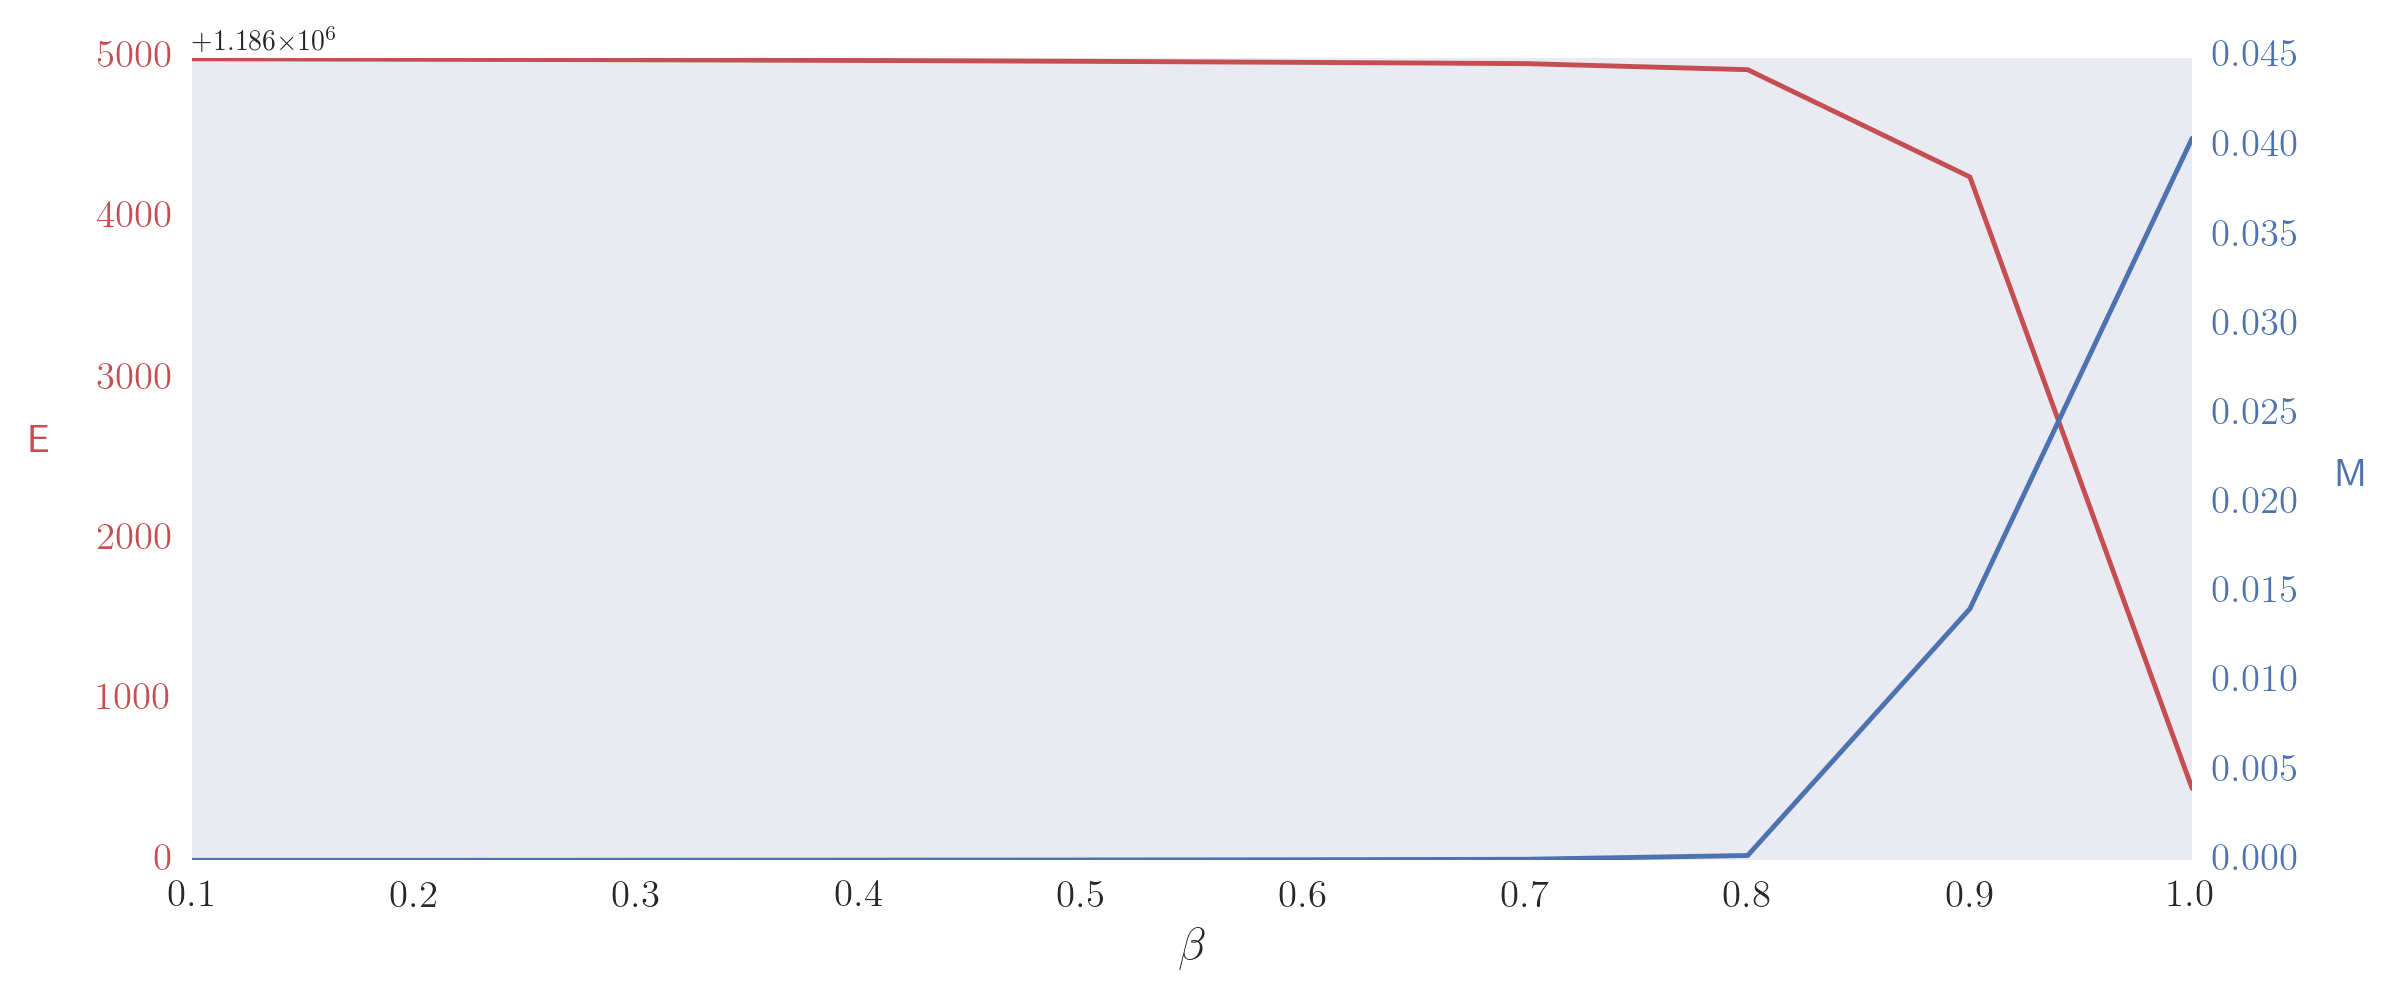
\includegraphics[width=\linewidth]{img/ising-energy-magnetization.png}
% }
% \caption{Energy (E) and magnetization (M) if the Ising spin model with
%   respect to the hyper-parameter $\beta$.}\label{snt:fig:ising-spin-em}
% \end{figure}

\begin{table}[h]
  \begin{center}
    \bgroup \setlength\tabcolsep{0.1\tabcolsep}\scriptsize
    \begin{tabular}{p{0.167\columnwidth} % first columm
        >{\centering\arraybackslash}p{0.057\columnwidth} % second columm
        *{9}{>{\centering\arraybackslash}p{0.07\columnwidth}} % next nine columns
        *{2}{>{\centering\arraybackslash}p{0.055\columnwidth}}} % last two columns
      \toprule
      \multirow{2}*{\bfseries Lexicon} & %
      \multirow{2}{0.06\columnwidth}{\bfseries \# of Terms} & %
      \multicolumn{3}{c}{\bfseries Positive Expressions} & %
      \multicolumn{3}{c}{\bfseries Negative Expressions} & %
      \multicolumn{3}{c}{\bfseries Neutral Terms} & %
      \multirow{2}{0.068\columnwidth}{\bfseries\centering Macro\newline \F{}} & %
      \multirow{2}{0.068\columnwidth}{\bfseries\centering Micro\newline \F{}}\\
      \cmidrule(lr){3-5}\cmidrule(lr){6-8}\cmidrule(lr){9-11}

      & & Precision & Recall & \F{} & %
      Precision & Recall & \F{} & %
      Precision & Recall & \F{} & & \\\midrule
      %% \multicolumn{9}{|c|}{\cellcolor{cellcolor}Existing Lexicons}\\\hline

      % Class                     Precision              Recall                 F-score
      % positive                   0.770601             0.101975                 0.180115
      % negative                   0.567901             0.017139                 0.033273
      % neutral                    0.963176             0.999227                 0.980870
      % Macro-average              0.767226             0.372780                 0.398086
      % Micro-average              0.962404             0.962216                 0.962310

      \textsc{Seed Set} & 20 & \textbf{0.771} & 0.102 & 0.18 & %
      \textbf{0.568} & 0.017 & 0.033 & %
      0.963 & \textbf{0.999} & \textbf{0.981} & %
      0.398 & \textbf{0.962}\\

      % Class                     Precision              Recall                 F-score
      % positive                   0.646220             0.133510                 0.221299
      % negative                   0.565217             0.029061                 0.055280
      % neutral                    0.964071             0.998134                 0.980807
      % Macro-average              0.725169             0.386902                 0.419129
      % Micro-average              0.962261             0.962072                 0.962167

      TKM & 920 & 0.646 & \textbf{0.134} & \textbf{0.221} & %
      0.565 & \textbf{0.029} & \textbf{0.055} & %
      \textbf{0.964} & 0.998 & \textbf{0.981} & %
      \textbf{0.419} & \textbf{0.962}\\

      % Class                     Precision              Recall                 F-score
      % positive                   0.764317             0.102269                 0.180400
      % negative                   0.567901             0.017139                 0.033273
      % neutral                    0.963181             0.999199                 0.980860
      % Macro-average              0.765133             0.372869                 0.398178
      % Micro-average              0.962384             0.962196                 0.962290

      VEL & 60 & 0.764 & 0.102 & 0.18 & %
      \textbf{0.568} & 0.017 & 0.033 & %
      0.963 & 0.999 & 0.98 & %
      0.398 & \textbf{0.962}\\

      % Class                     Precision              Recall                 F-score
      % positive                   0.386437             0.105806                 0.166127
      % negative                   0.567901             0.017139                 0.033273
      % neutral                    0.963178             0.996092                 0.979359
      % Macro-average              0.639172             0.373012                 0.392920
      % Micro-average              0.959478             0.959290                 0.959384

      KIR & 320 & 0.386 & 0.106 & 0.166 & %
      \textbf{0.568} & 0.017 & 0.033 & %
      0.963 & 0.996 & 0.979 & %
      0.393 & 0.959\\

      % Class                     Precision              Recall                 F-score
      % positive                   0.679764             0.101975                 0.177345
      % negative                   0.567901             0.017139                 0.033273
      % neutral                    0.963162             0.998820                 0.980667
      % Macro-average              0.736942             0.372644                 0.397095
      % Micro-average              0.962013             0.961825                 0.961919

      SEV & 60 & 0.68 & 0.102 & 0.177 & %
      \textbf{0.568} & 0.017 & 0.033 & %
      0.963 & \textbf{0.999} & \textbf{0.981} & %
      0.397 & \textbf{0.962}\\

      TKM $\cap$ VEL $\cap$ SEV & 20 & \textbf{0.771} & 0.102 & 0.18 & %
      \textbf{0.568} & 0.017 & 0.033 & %
      0.963 & \textbf{0.999} & \textbf{0.981} & %
      0.398 & \textbf{0.962}\\

      % Class                     Precision              Recall                 F-score
      % positive                   0.592689             0.133805                 0.218322
      % negative                   0.565217             0.029061                 0.055280
      % neutral                    0.964063             0.997700                 0.980593
      % Macro-average              0.707323             0.386855                 0.418065
      % Micro-average              0.961850             0.961662                 0.961756

      TKM $\cup$ VEL $\cup$ SEV & 1,020 & 0.593 & \textbf{0.134} & 0.218  & %
      0.565 & \textbf{0.029} & \textbf{0.055} & %
      \textbf{0.964} & 0.998 & 0.98 & %
      0.418 & \textbf{0.962}\\\bottomrule
    \end{tabular}
    \egroup
    \caption[Results of corpus-based approaches]{Results of
      corpus-based approaches\\ {\small TKM -- \citet{Takamura:05},
        VEL -- \citet{Velikovich:10}, KIR -- \citet{Kiritchenko:14},
        SEV -- \citet{Severyn:15}}}
    \label{snt-lex:tbl:corp-meth}
  \end{center}
\end{table}

The results of this evaluation are presented in
Table~\ref{snt-lex:tbl:corp-meth}.  This time, we can observe a clear
superiority of the system of~\citet{Takamura:05}, which not only
achieves the best recall and \F{}-value on recognizing positive and
negative terms, but also yields the highest micro- and macro-averaged
results on all three polarity classes.
% As expected, the best precision in recognizing polar terms is achieved
% by the manually compiled seed set, whose micro-averaged \F{}-result,
% however, is still identical to the one shown by the method of
% \citet{Takamura:05}.
The size and scores of the other lexicons, however, are much smaller
than the cardinalities and results obtained by the dictionary-based
methods and the Takamura et al.'s approach.  Moreover, those polarity
lists also show absolutely identical performance on the negative class
as the original seed set.

Since the last results were somewhat unexpected, we decided to
investigate the reasons for potential problems in these systems.  A
closer look at the learning curves of these methods revealed that
their macro-averaged \F{}-values on the held-out development set were
rapidly going down as the number of the included polar entries
increased.  Since we considered the lexicon size as one of the
hyper-parameters of the tested approaches, we rapidly stopped
populating these lists after noticing a decrease of their results.  As
a consequence, only few highest ranked terms (all of which were
positive) were included into the final resources.  As it turned out
the main reason for this positive bias of the top-scoring entries was
the ambiguity of the utilized seed set: While adapting the original
seed list of~\citet{Turney:03} to German, we translated the English
word ``correct'' as ``richtig''.  This German word, however, also has
another reading, viz., \emph{real} (as in ``ein richtiges Spiel''
\emph{a real game} or ``ein richtiger Rennwagen'' \emph{a real sports
  car}), which was much more frequent in the analyzed snapshot, often
appearing in a negative context, e.g., ``ein richtiger
Bombenanschlag'' (\emph{a real bomb attack}) or ``ein richtiger
Terrorist'' (\emph{a real terrorist}).  As a consequence, methods
relying on distant supervision had to deal with an extremely
unbalanced training set,\footnote{The automatically labeled corpus
  that we obtained for the approach by \citet{Kiritchenko:14} using
  these seeds, for instance, had 716,210 positive versus 92,592
  negative training instances.} and fell victim to this unjustified
skewness, getting stuck in a local optimum from the very beginning of
their training.\footnote{Later, in Section~\ref{subsec:snt-lex:eoss},
  we will investigate whether alternative seed sets proposed by other
  authors could provide a remedy to the above problem.}

\subsection{NWE-Based Methods}\label{subsec:snt:lex:nwe}

Finally, the last group of SLG methods that we are going to explore in
this section are algorithms which operate on distributed vector
representations of words---neural word embeddings (NWEs).  First
introduced by~\citet{Bengio:03} and further refined by
\citet{Collobert:11} and \citet{Mikolov:13}, NWEs had a great
``tsunami''-like effect on many downstream NLP
applications~\cite{Manning:15}.  Unfortunately, to this day, the SLG
task remained mainly untouched from these advances, up to a few
exceptional works introduced by~\citet{Tang:14a} and \citet{Vo:16}.
In the former approach, the authors used a large collection of noisily
labeled tweets\footnote{Similarly to the corpus-based approaches
  of~\citet{Kiritchenko:14} and \citet{Severyn:15a}, the authors
  assigned polarity labels to the messages based on the occurrence of
  positive and negative smileys in these tweets.}  in order to learn
hybrid word embeddings.  In contrast to the standard word2vec
vectors~\cite{Mikolov:13} and purely task-specific
representations~\cite{Collobert:11}, such embeddings were trained to
optimize both objectives---predicting the co-occurrence of other words
in the nearby context, and classifying the polarity type of the whole
messages.  In the next step, \citet{Tang:14a} trained a simple
one-layer feed-forward neural network on the aforementioned hybrid
vectors, trying to predict the noisy labels of the messages, and
applied this classifier separately to each embedding, considering the
predicted score as the polarity value of the respective word or
phrase.  Similarly, \citet{Vo:16} also adopted the distant supervision
framework.  However, in contrast to the former method, they ab initio
trained two-dimensional task-specific representations, and regarded
the two elements of the learned vectors as positive and negative
scores of the respective words.

In order to estimate the potential of these systems for an automatic
generation of sentiment lexicons for German Twitter, we again
reimplemented these approaches, extending them to three-way
classification (positive, negative, and neutral), and applied them to
distantly labeled tweets introduced in the previous sections.

In addition to that, we also came up with four alternative ways of
generating polarity lists from NWEs:
\begin{itemize}
\item the method of the nearest centroids,
\item the $k$-NN algorithm;
\item the principal component analysis,
\item and the linear projection approach.
\end{itemize}

With the first method, we used the embeddings of the seed terms to
compute the centroids of the positive, negative, and objective
clusters.  Afterwards, we assigned a new word $w$ to the polarity
group whose centroid was the closest to its vector.  We considered the
distance to the cluster center as the polarity score of the included
word, and sorted the resulting sentiment lexicon in the ascending
order of these values.

Similarly, with the $k$-NN algorithm, for every new word $w$, we
looked for $k$ seed embeddings that were closest to the $w$'s vector,
and allocated this term to the polarity class whose seeds were nearest
and appeared most frequently in its neighborhood.

\begin{algorithm}
  \begin{algorithmic}[1]
    \Function{ExpandPCA}{$\mathcal{P}, \mathcal{N}, \mathcal{O}, \vars{E}$}\Comment{$\mathcal{P}$~--~indices of positive terms,}
    \Statex\Comment{$\mathcal{N}$~--~indices of negative terms,}
    \Statex\Comment{$\mathcal{O}$~--~indices of objective terms, $\vars{E}$~--~embedding matrix}
    \State $\vars{U}, \Sigma, \vars{V}^\top\gets\func{SVD}(\vars{E})$;\Comment{obtain singular components of \vars{E}}
    \State $\vars{E}'\gets\left(\vars{E}^\top\cdot \vars{U}\right)^\top$;\Comment{project \vars{E} onto the eigenvectors of its row space}
    \State $\mathcal{S}\gets\mathcal{P}\cup\mathcal{N}$;\Comment{get the set of subjective terms}
    \State $\vars{u}_{subj}, \mu_{\mathcal{S}}, \mu_{\mathcal{O}}\gets\func{FindMeanAxis}(\vars{E}', \mathcal{S}, \mathcal{O})$;\Comment{find
      subjectivity axis}
    \State $\vars{u}_{pol}, \mu_{\mathcal{P}}, \mu_{\mathcal{N}}\gets\func{FindAxis}(\vars{E}', \mathcal{P}, \mathcal{N})$;\Comment{find polarity axis}
    \State\Return $\func{ComputePolScores}(\vars{E}', \mathcal{S}\cup\mathcal{O},%
    \vars{u}_{subj}, \vars{u}_{pol}, \mu_{\mathcal{S}}, \mu_{\mathcal{O}},%
    \mu_{\mathcal{P}}, \mu_{\mathcal{N}})$;
    \EndFunction
    \Statex
    \Function{FindMeanAxis}{$\vars{E}, \mathcal{S}_1, \mathcal{S}_2$}
    \State $\mu_1\gets 0$; $\mu_2\gets 0$; \vars{axis} $\gets 0$; \vars{max\_dist} $\gets 0$;
    \For{$\vars{i}\gets 1$; $\vars{i} <= \func{nrows}(\vars{E})$; $\vars{i}\gets\vars{i} + 1$}
    \State \vars{e} $\gets$\vars{M[i]};
    \State \vars{dist} $\gets\sum_{j_1\in\mathcal{S}_1,j_2\in\mathcal{S}_2}\left|\vars{e}[j_1] - \vars{e}[j_2]\right|$;
    \If {\vars{dist} $>$ \vars{max\_dist}}
    \State \vars{axis} $\gets$\vars{i}; \vars{max\_dist} $\gets$ \vars{dist};
    \State $\mu_1\gets\frac{\sum_{j_1\in\mathcal{S}_1}\vars{e}[j_1]}{|\mathcal{S}_1|}$; $\mu_2\gets\frac{\sum_{j_2\in\mathcal{S}_2}\vars{e}[j_2]}{|\mathcal{S}_2|}$;
    \EndIf
    \EndFor
    \State\Return\vars{axis}, $\mu_1$, $\mu_2$;
    \EndFunction
    \Statex
    \Function{ComputePolScores}{$\vars{E}, \mathcal{S}, \vars{u}_{subj}, \vars{u}_{pol},
      \mu_{\mathcal{S}}, \mu_{\mathcal{O}}, \mu_{\mathcal{P}}, \mu_{\mathcal{N}}$}
    \State\vars{scores} $\gets []$;

    \State\vars{O}$_{subj}\gets\mu_{\mathcal{O}} + \frac{\mu_{\mathcal{S}} -
    \mu_{\mathcal{O}}}{2}$;\Comment{Compute the origin of the
      subjectivity axis.}

    \State\vars{max\_score}$_{subj}\gets\max\left(\{|\vars{n}\lbrack\vars{u}_{subj}\rbrack%
      - \vars{O}_{subj}| |\forall\vars{n}\in\func{cols}(\vars{E})\}\right)$;

    \State\vars{O}$_{pol}\gets\mu_{\mathcal{N}} + \frac{\mu_{\mathcal{P}} -
    \mu_{\mathcal{N}}}{2}$;\Comment{Compute the origin of the polarity
      axis.}

    \State\vars{max\_score}$_{pol}\gets\max\left(\{|\vars{n}\lbrack\vars{u}_{pol}\rbrack%
      - \vars{O}_{pol}| |\forall\vars{n}\in\func{cols}(\vars{M})\}\right)$;

    \For{$\vars{i}\gets 1$; $\vars{i} <= \func{ncols}(\vars{M})$; $\vars{i}\gets\vars{i} + 1$}
    \If {$\vars{i} \in \mathcal{S}$}
    \State \textbf{continue};\Comment{known seeds will be added later by default}
    \EndIf
    \State \vars{n}$\gets$\vars{M[:, i]}$^\top$;\Comment{assign $i$-th column to \vars{n}}

    \If {$|\vars{n}\lbrack\vars{u}_{subj}\rbrack - \mu_{\mathcal{O}}| > %
      |\vars{n}\lbrack\vars{u}_{subj}\rbrack - \mu_{\mathcal{S}}|$}%
    \Comment{if the $i$-th word is subjective}

    \State\vars{score}$_{subj}\gets 1 + %
    \frac{|\vars{n}\lbrack\vars{u}_{subj}\rbrack - \vars{O}_{subj}|}{\vars{max\_score}_{subj}}$;
    \algstore{sentilex-pca}
  \end{algorithmic}
  \caption[Sentiment lexicon generation using PCA]{Sentiment lexicon
    generation with the PCA algorithm}\label{snt:lex:alg:pca}
\end{algorithm}

\begin{algorithm}
  \begin{algorithmic}[1]
    \algrestore{sentilex-pca}
    \Else
    \State\vars{score}$_{subj}\gets 1 - %
    \frac{|\vars{n}\lbrack\vars{u}_{subj}\rbrack - \vars{O}_{subj}|}{\vars{max\_score}_{subj}}$;
    \EndIf

    \If {$|\vars{n}\lbrack\vars{u}_{pol}\rbrack - \mu_{\mathcal{N}}| > %
      |\vars{n}\lbrack\vars{u}_{pol}\rbrack - \mu_{\mathcal{P}}|$}%
    \Comment{if the $i$-th word is positive}

    \State\vars{polarity}$\gets$ positive;
    \Else
    \State \vars{polarity}$\gets$ negative;
    \EndIf
    \State\vars{score}$_{pol}\gets%
    \frac{|\vars{n}\lbrack\vars{u}_{pol}\rbrack %
      - \vars{O}_{pol}|}{\vars{max\_score}_{pol}}$;
    \State\func{append}(\vars{scores},
    (\vars{i}, \vars{polarity}, %
    $\frac{1}{\vars{score}_{\textrm{subj}} + \vars{score}_{pol}}$));\Comment{The total score is inversed}
    \Statex\Comment{as we sort the resulting polarity list in the ascending order.}
    \EndFor
    \State\Return\vars{scores};
    \EndFunction
  \end{algorithmic}
\end{algorithm}

A slightly different technique was used with the approach of the
principal component analysis.  After normally decomposing the
embedding matrix~$E\in\mathbb{R}^{d\times|V|}$ (with $d$ denoting the
dimension of the word vectors (in our case $d = 300$),\footnote{Due to
  implementation specifics, the initial embedding vectors had to be
  represented as columns.} and $|V|$ representing the vocabulary size)
into its singular components:
\begin{align*}
  E = U \Sigma V^T,
\end{align*}
where the matrices $U$ and $V$ stand for the orthogonal bases of the
row and column spaces of $E$ respectively, we looked for the row axis
$u\in U$ such that the embeddings of the seed terms with opposite
semantic orientations projected on this axis would be maximally far
apart from each other.

We first applied this method to find an axis $u_{\textrm{subj}}$ which
maximized the distance between the projections of subjective (positive
and negative) and neutral terms; and then used the same procedure to
determine an axis $u_{\textrm{pol}}$ such that the projections of
positive and negative terms on this line would be furthest away from
each other.  Considering the distances to the origins of these axes as
subjectivity and polarity scores of the projected words respectively,
we estimated the final lexicon score of the newly added terms as the
inverse sum of these values (i.e., one over the sum of both
distances), and sorted the resulting list in the ascending order.  The
pseudo-code of this approach is shown in
Algorithm~\ref{snt:lex:alg:pca}.

Since PCA, however, was not guaranteed to find the optimum polarity
axis (the orthogonal bases in SVD are typically computed using the
covariance matrix of $E$, and might therefore fail to capture semantic
orientations if terms with opposite polarities occur in similar
contexts), we additionally introduced our own \emph{linear projection
  method}, in which we explicitly adopted the aforementioned
objective: Namely, given two sets of vectors with opposite semantic
orientations (let us, for instance, denote the set of positive vectors
as~$\mathcal{P} = \{\vec{p}_{+_1},\ldots,\vec{p}_{+_m}\}$, and the set
of negative embeddings
as~$\mathcal{N} = \{\vec{p}_{-_1},\ldots,\vec{p}_{-_n}\}$), find a
projection line $\vec{b}$ which would maximize the distance between
the projections of the terms from these disjoint seed sets, i.e.:
{\small%
\begin{align}
  \small
  \vec{b} &=\argmax\frac{1}{2}\sum_{\vec{p}_+}\sum_{\vec{p}_-}%
  \left\lVert\frac{\vec{b}\cdot\vec{p}_+}{\vec{b}^2}\vec{b}%
  - \frac{\vec{b}\cdot\vec{p}_-}{\vec{b}^2}\vec{b}\right\rVert^2\\
  &=\argmax\frac{1}{2}\sum_{\vec{p}_+}\sum_{\vec{p}_-}\left\lVert\frac{\vec{b}%
    \cdot\left(\vec{p}_{+}-\vec{p}_{-}\right)}{\vec{b}^2}\vec{b}\right\rVert^2,\label{eq:f}%
\end{align}\normalsize}%
where $\frac{\vec{b}\cdot\vec{p}_+}{\vec{b}^2}\vec{b}$ is the
projection of a word embedding with the positive polarity on the line
$\vec{b}$, and $\frac{\vec{b}\cdot\vec{p}_-}{\vec{b}^2}\vec{b}$ is the
respective projection of a negative seed term.

% (see Figure~\ref{fig:linproj.L.M} for a visual explanation of this
% method).\footnote{Since we are only interested in finding the slope of
%   the projection line, we assume an intercept of zero.}

Considering the $\argmax$ argument in Expression~\ref{eq:f} as the
objective function~$f$, we can compute the gradient of~$f$ with
respect to~$\vec{b}$ as follows:

{\small%
  \begin{align}
    \nabla f &= \sum_{\vec{p}_+}\sum_{\vec{p}_-}%
               \gamma\left(\Delta - \gamma\vec{b^{i}}\right),\label{eq:prj-line-grad}%
\end{align}\normalsize}%
where $\Delta$ stands for the difference between the positive and
negative vectors~$\vec{p}_{+}$ and~$\vec{p}_{-}$:
$\Delta = \vec{p}_{+}-\vec{p}_{-}$; and $\gamma$ denotes the dot
product of this difference with the projection vector~$\vec{b}$ at the
$i$-th iteration step: $\gamma = \Delta \cdot \vec{b}^i$.\footnote{A
  detailed explanation of the gradient computation is given in
  Appendix~\ref{chap:apdx:lex-grad} of this thesis.}  With this
gradient, we can easily optimize the vector~$\vec{b}$ using gradient
ascent until we reach the global maximum of the function~$f$.

% \begin{minipage}{0.4\textwidth}
%   \centering
%   \mbox{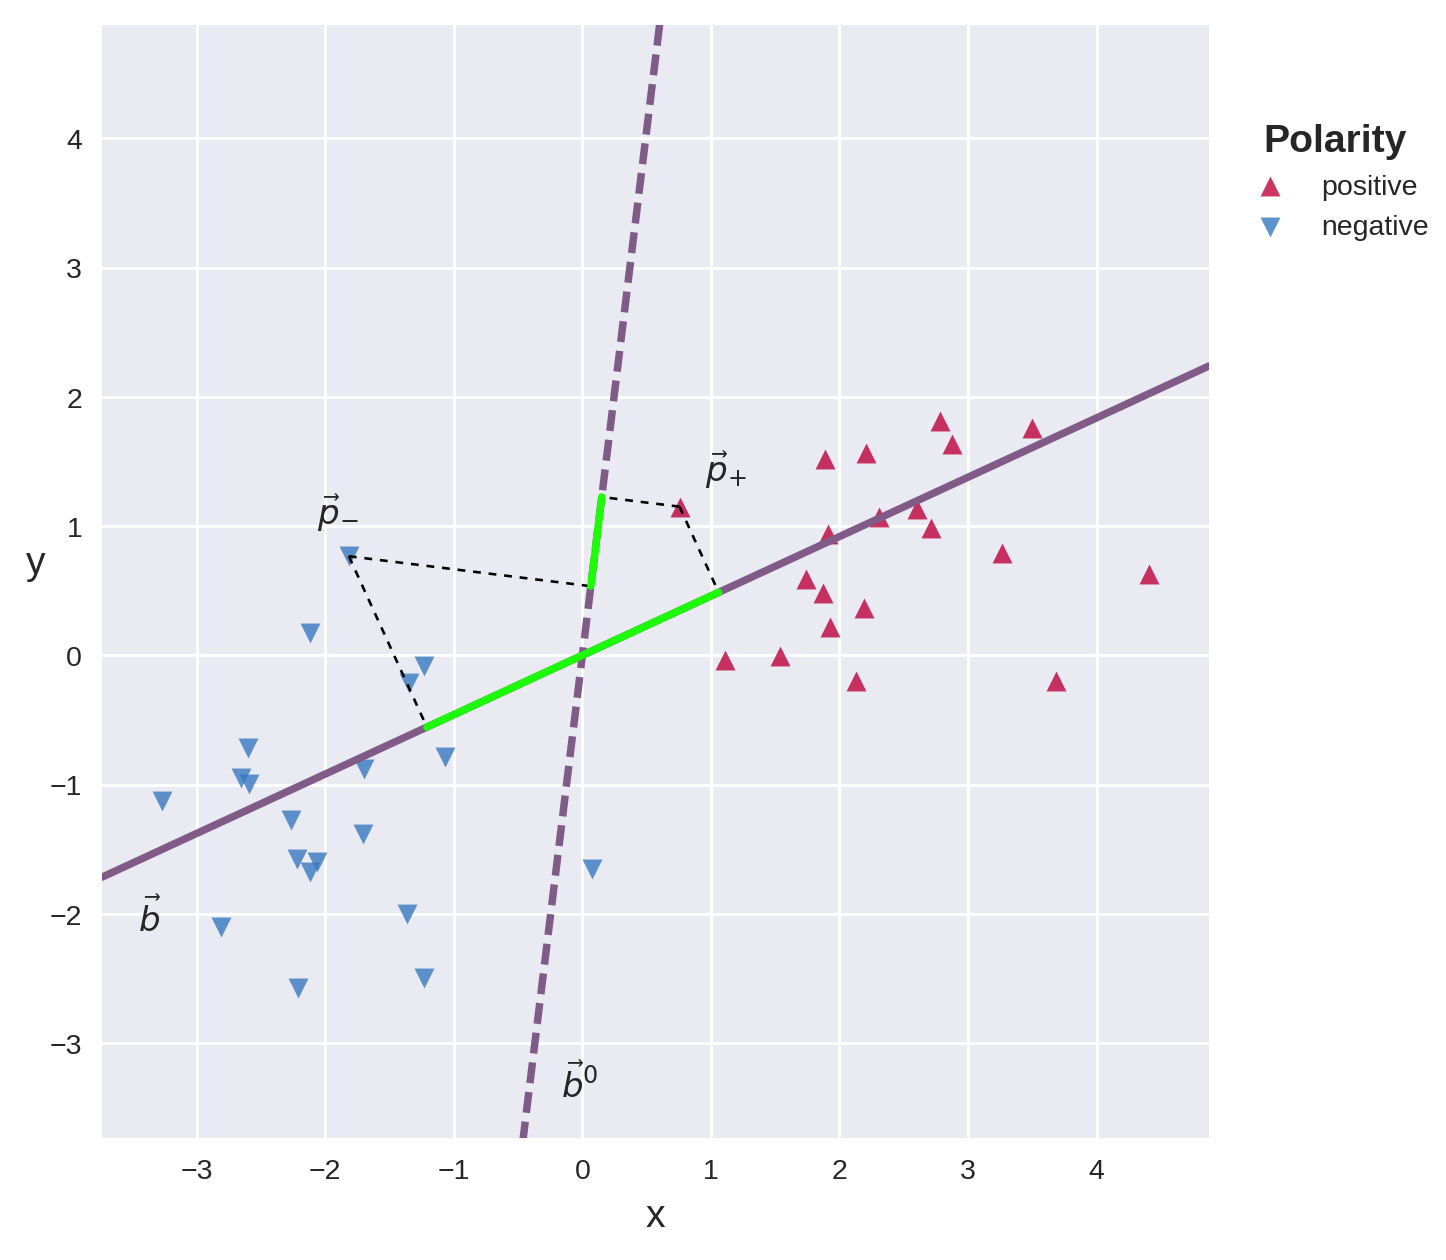
\includegraphics[height=15em]{img/sentilex_L_M}}
%   \captionof{figure}[A visualization of the linear projection method in a
%   two-dimensional vector space.]{A visualization of the linear
%     projection method in a
%     two-dimensional vector space.\\
%     (\small$\vec{b}^0$ --- initial guess of the projection line;
%     $\vec{b}$ --- optimal projection vector; the distances between the
%     respective projections of two sample seeds with opposite semantic
%     orientations ($p^+$ and $p^-$) on these lines are highlighted in
%     \textcolor{highlighter green}{green})}
%   \label{fig:linproj.L.M}
% \end{minipage}

% After determining the optimal line~$\vec{b}$, we projected all known
% word embeddings on the slope of this vector, and determined its origin
% point~$O_{\vec{b}}$, which not necessarily had to be identical with
% the global origin~$O$ of the initial coordinate system: {\small%
%   \begin{align}
%     O_{\vec{b}} &= \mu_- + \frac{\mu_+ - \mu_-}{2}.
% \end{align}\normalsize}%
% The~$\mu_-$ term in the above equation represents the mean of the
% projected embeddings of the negative seed terms:
% $\mu_- = \frac{\sum\vec{p'_-}}{|\mathcal{N}|}$; and the~$\mu_+$
% variable stands for the respective mean of the projections of positive
% seeds.  % With this origin, we finally computed the subjectivity and
% % polarity scores of the remaining terms with unknown semantic
% % orientations.

Similarly to the PCA method, we first applied this approach to
determine the optimal subjectivity axis $\vec{b}_{subj}$ which
maximized the mutual distance between the sets of subjective and
objective words, and then computed the subjectivity scores for polar
and neutral terms
as~$s^{pol}_{subj} = 1 + \frac{\delta_{subj}^i}{\delta_{subj}^{\max}}$
and
$s^{neut}_{subj} = 1 - \frac{\delta_{subj}^i}{\delta_{subj}^{\max}}$
respectively, where $\delta_{subj}^i$ stands for the distance between
the projection of the $i$-th term and the origin $O_{subj}$, and
$\delta_{subj}^{\max}$ denotes the maximum such distance observed in
the data.

Afterwards, we estimated the polarity scores by first finding a
projection line~$\vec{b}_{pol}$ with the maximum difference between
the projected positive and negative seeds; then computing the origin
of this line~$O_{pol}$; and, finally, calculating the polarity value
of the $i$-th term
as~$s_{pol} = 1 + \frac{\delta^i_{pol}}{\delta^{max}_{pol}}$.

\begin{figure*}[hbt!]
  \centering
  \begin{subfigure}{.45\textwidth}
    \centering
    \mbox{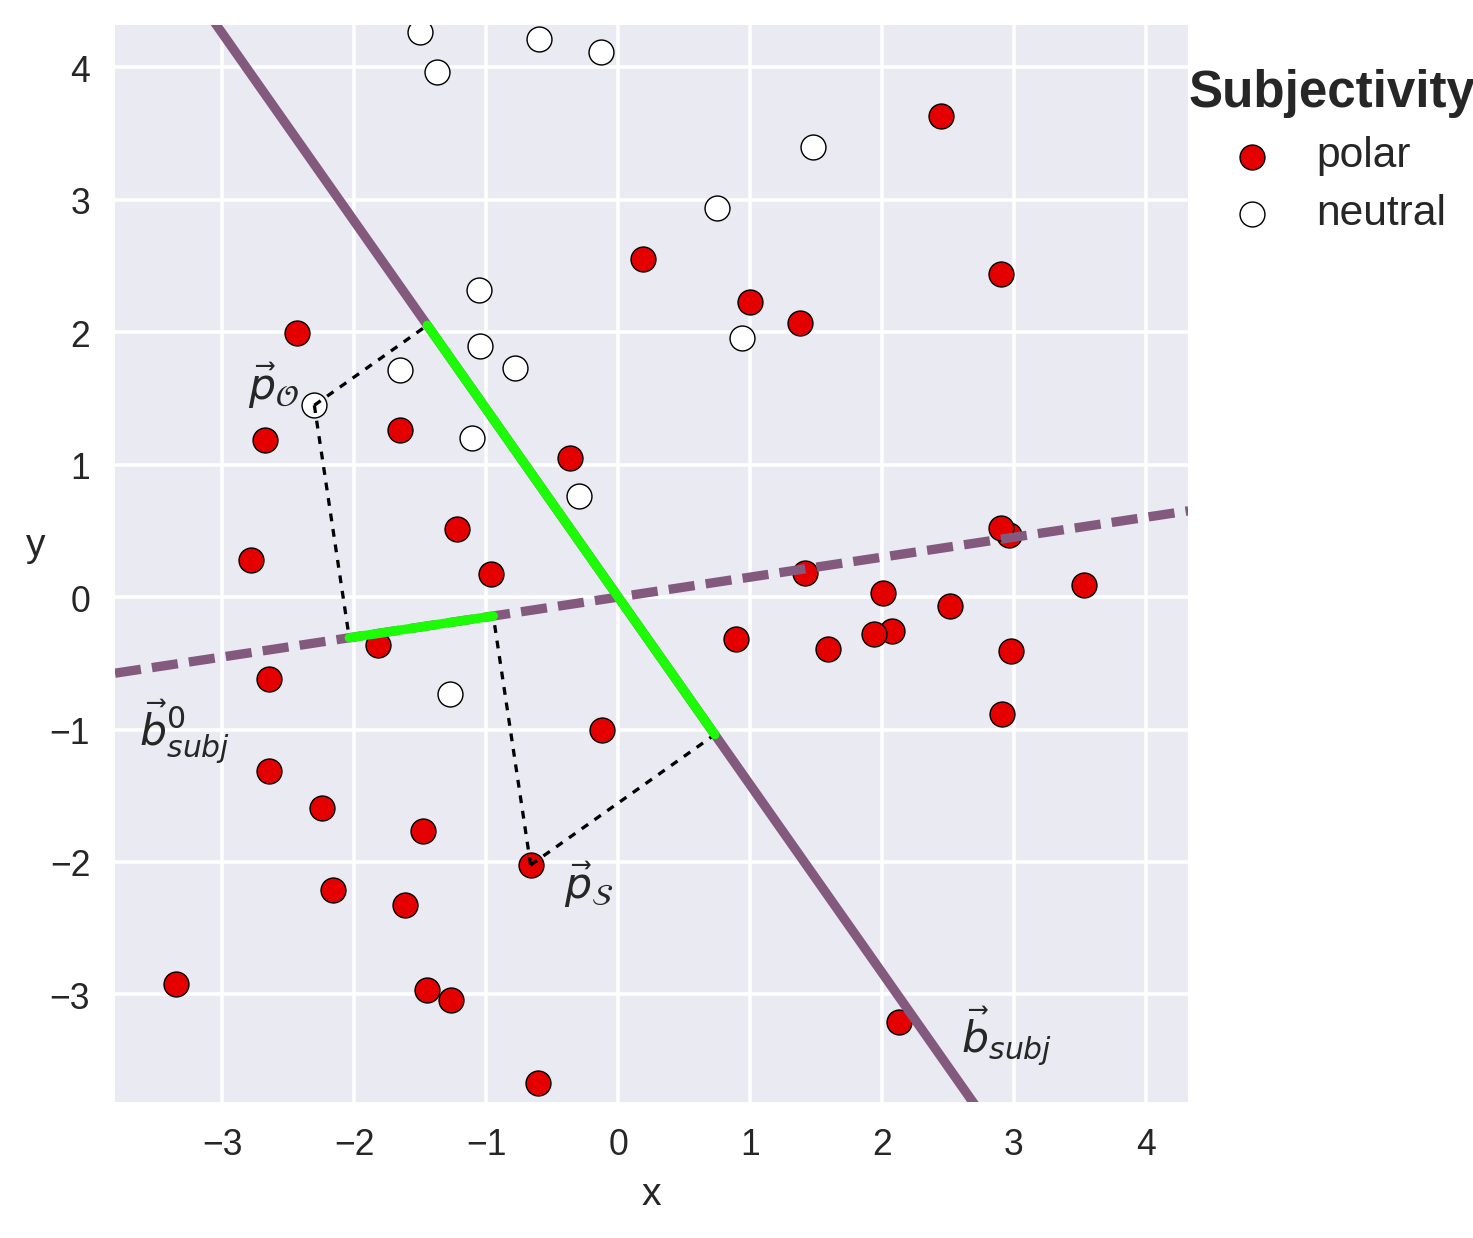
\includegraphics[height=15em]{img/sentilex_subjectivity}}
    \caption{Subjectivity line}
  \end{subfigure}
  \begin{subfigure}{.45\textwidth}
    \centering
    \mbox{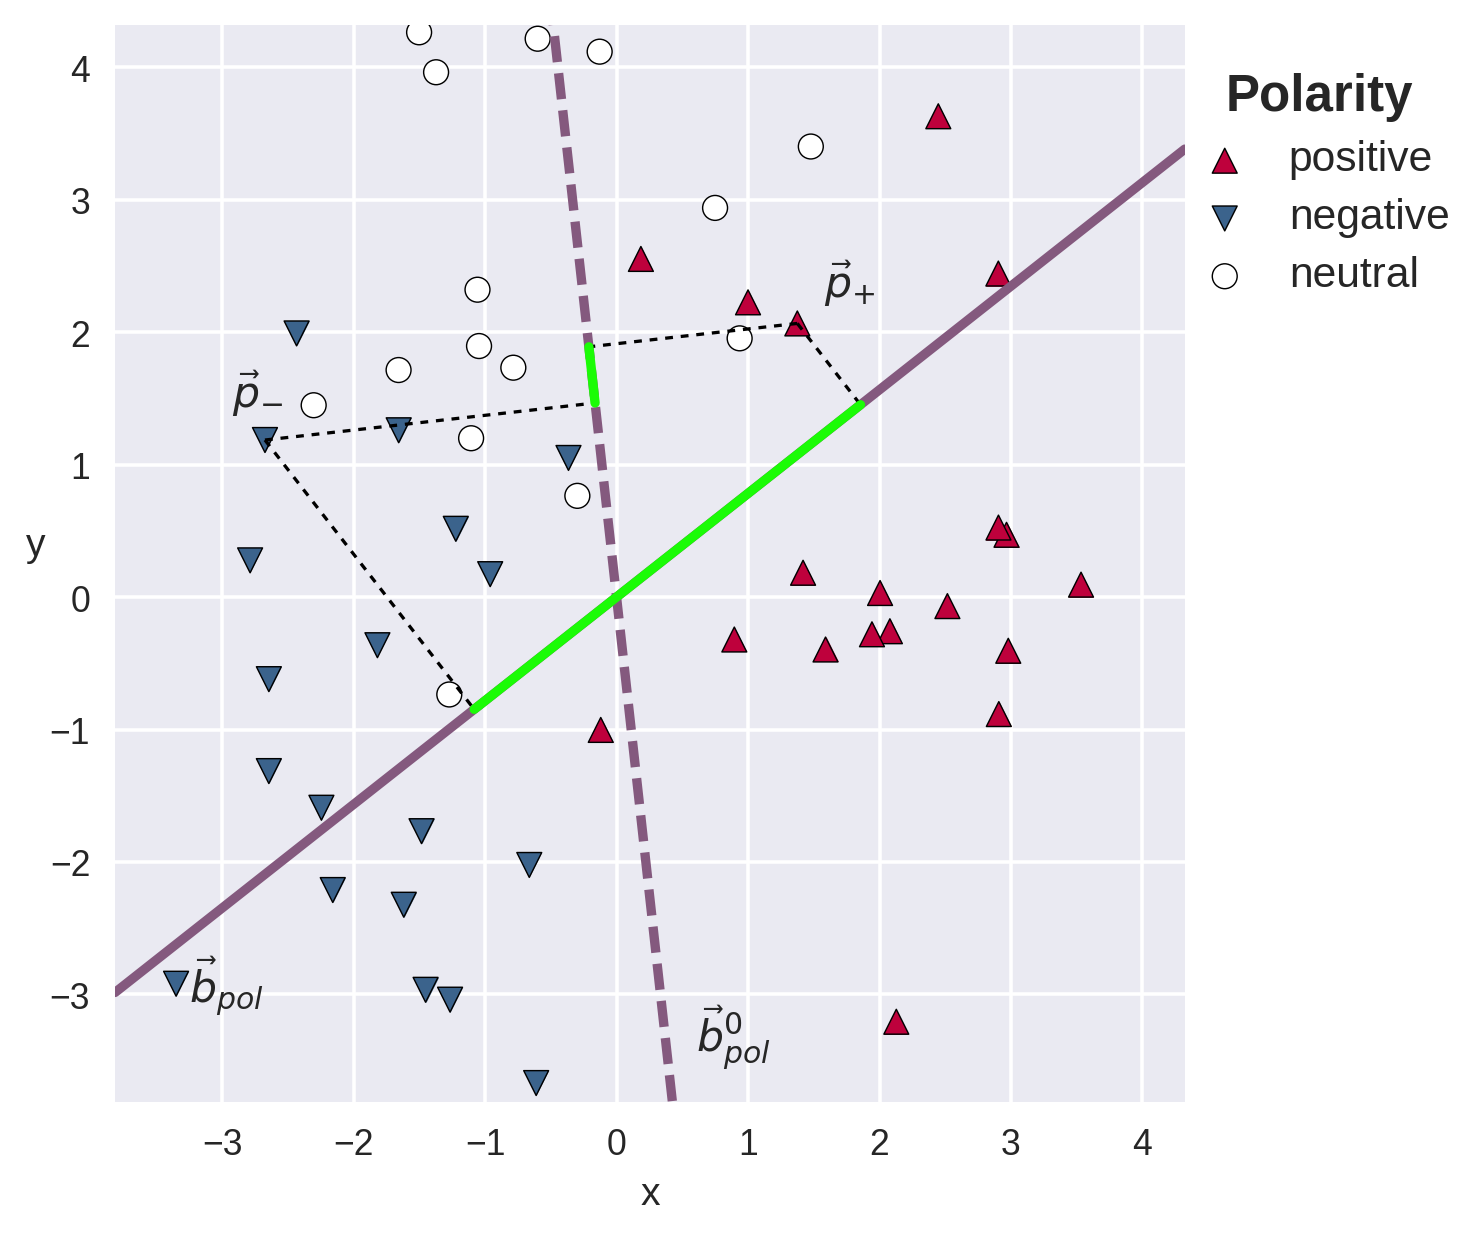
\includegraphics[height=15em]{img/sentilex_polarity}}
    \caption{Polarity line}
  \end{subfigure}
  \caption[Visualization of the linear projection method in the
  two-dimensional vector space]{Visualization of the linear
    projection method in the
    two-dimensional vector space with unnormalized vectors\\
    (\small $\vec{b}^0_{subj}$ and $\vec{b}^0_{pol}$~--~initial
    guesses of the subjectivity and polarity lines; $\vec{b}_{subj}$
    and $\vec{b}_{pol}$~--~optimal projection vectors; the distances
    between the projections of sample seeds with opposite semantic
    orientations ($\vec{p}_{\mathcal{S}}$ vs. $\vec{p}_{\mathcal{O}}$
    and $\vec{p}_+$ vs. $\vec{p}_\_$ respectively) on these lines are
    highlighted in \textcolor{highlighter green}{green})}
  \label{fig:linproj}
\end{figure*}

In the concluding step, we joined the two score types (subjectivity
and polarity) as described above: $s = \frac{1}{s_{subj} + s_{pol}}$,
and, again, sorted the resulting list in the ascending order of these
ranks.  The pseudo-code of this approach is shown in
Algorithm~\ref{snt:lex:alg:linproj}, and a visualization of the line
optimization step (in the two-dimensional vector space with
unnormalized vectors) is provided in Figure~\ref{fig:linproj}.

\begin{algorithm}
  \begin{algorithmic}[1]
    \Function{ExpandLinProj}{$\mathcal{P}, \mathcal{N}, \mathcal{O}, \vars{E}$}\Comment{$\mathcal{P}$~--~indices of positive terms,}
    \Statex\Comment{$\mathcal{N}$~--~indices of negative terms,}
    \Statex\Comment{$\mathcal{O}$~--~indices of objective terms, $\vars{E}$~--~embedding matrix}
    \State $\mathcal{S}\gets\mathcal{P}\cup\mathcal{N}$;\Comment{get the set of subjective terms}
    \State $\vars{proj}_{subj}, \mu_{\mathcal{S}}, \mu_{\mathcal{O}}\gets%
    \func{Project}(\mathcal{S}, \mathcal{O}, \vars{E})$;
    \State $\vars{proj}_{pol}, \mu_{\mathcal{P}}, \mu_{\mathcal{N}}%
    \gets\func{Project}(\mathcal{P}, \mathcal{N}, \vars{E})$;
    \State\Return $\func{ComputePolScores}(\vars{E}, \mathcal{S}\cup\mathcal{O},%
    \vars{proj}_{subj}, \vars{proj}_{pol}, %
    \mu_{\mathcal{S}}, \mu_{\mathcal{O}}, \mu_{\mathcal{P}}, \mu_{\mathcal{N}})$;
    \EndFunction
    \Statex
    \Function{Project}{$\mathcal{S}_1, \mathcal{S}_2, \vars{E}$}
    \State $\vars{projs}\gets []$, $\mu_1\gets \vec{0}$; $\mu_2\gets \vec{0}$;
    \State $\vec{b}\gets\func{FindAxis}(\mathcal{S}_1, \mathcal{S}_2)$;\Comment{Determine the optimum polarity/subjectivity axis}
    \For{$\vars{i}\gets 1$; $\vars{i} <= \func{nrows}(\vars{E})$; $\vars{i}\gets\vars{i} + 1$}
    \State $\vec{p}\gets\vec{b}*\vars{E}$[$i$]$\cdot\vec{b}$;\Comment{Project $i$-th embedding onto the axis}
    \State $\func{append}(\vars{projs}, \vec{p})$;
    \If{$\vars{j}\in\mathcal{S}_1$}\Comment{Update means of the polarity/subjectivity classes}
    \State $\mu_1\gets\mu_1 + \vec{p}$;
    \Else
    \If{$\vars{k}\in\mathcal{S}_2$}
    \State $\mu_2\gets\mu_2 + \vec{p}$;
    \EndIf
    \EndIf
    \EndFor
    \State\Return $\vars{projs}$, $\frac{\mu_1}{|\mathcal{S}_1|}$; $\frac{\mu_2}{|\mathcal{S}_2|}$;
    \EndFunction
    \Statex
    \Function{FindAxis}{$\mathcal{S}_1, \mathcal{S}_2, \vars{E}$}
    \State $\vec{b}\gets\vec{1}$; $\vars{prev\_dist}\gets \infty$;
    \For{$\vars{i}\gets 1$; $\vars{i} \leqslant \vars{MAX\_ITERS}$; $\vars{i}\gets\vars{i} + 1$}
    \State $\vec{b}\gets\frac{\vec{b}}{\norm{\vec{b}}}$;\Comment{Ensure the projection line
      has a unit length}
    \State$\vars{dist}\gets 0$;
    \For{$\vars{j}\in\mathcal{S}_1$}
    \State $\vec{p}_1\gets\vec{b}*\vars{E}$[$j$]$\cdot\vec{b}$;\Comment{Project a seed term from the first set}
    \For{$\vars{k}\in\mathcal{S}_2$}
    \State $\vec{p}_2\gets\vec{b}*\vars{E}$[$k$]$\cdot\vec{b}$;\Comment{Project a seed term from the second set}
    \State$\vars{dist}\gets \vars{dist} + \norm{\vec{p}_1 - \vec{p}_2}$;\Comment{Accumulate the distance}
    \Statex\Comment{between the two projections}
    \EndFor
    \EndFor
    \algstore{sentilex-linproj-1}
  \end{algorithmic}
  \caption[Sentiment lexicon generation using linear
  projection]{Sentiment lexicon generation with the linear projection
    algorithm}\label{snt:lex:alg:linproj}
\end{algorithm}

\begin{algorithm}
  \begin{algorithmic}[1]
    \algrestore{sentilex-linproj-1}
    \If{$\vars{prev\_dist}\neq\infty$ \textbf{and} $\vars{dist} - \vars{prev\_dist} < \epsilon$}
    \State\textbf{break};\Comment{Break if the convergence criterion was reached}
    \EndIf
    \State $\vars{prev\_dist}\gets\vars{dist}$;
    \State $\vec{b}\gets\vec{b} + \alpha*\nabla\vec{b}$;\Comment{Optimize the projection line}
    \EndFor
    \State\Return $\vec{b}$;
    \EndFunction
    \Statex
    \Function{ComputePolScores}{$\vars{E}, \mathcal{S}, \vars{projections}_{subj}, %
      \vars{projections}_{pol}, \mu_{\mathcal{S}}, \mu_{\mathcal{O}}, %
      \mu_{\mathcal{P}}, \mu_{\mathcal{N}}$}
    \State\vars{scores} $\gets []$;

    \State\vars{O}$_{subj}\gets\mu_{\mathcal{O}} + \frac{\mu_{\mathcal{S}} -
    \mu_{\mathcal{O}}}{2}$;\Comment{Compute the origin of the
      subjectivity axis.}

    \State\vars{max\_score}$_{subj}\gets\max\left(\{|\vars{p}_{subj}%
      - \vars{O}_{subj}| |\forall\vars{p}_{subj}\in\vars{projections}_{subj}\}\right)$;

    \State\vars{O}$_{pol}\gets\mu_{\mathcal{N}} + \frac{\mu_{\mathcal{P}} -
    \mu_{\mathcal{N}}}{2}$;\Comment{Compute the origin of the polarity
      axis.}

    \State\vars{max\_score}$_{pol}\gets\max\left(\{|\vars{p}_{pol}%
      - \vars{O}_{pol}| |\forall\vars{p}_{pol}\in\vars{projections}_{pol}\}\right)$;

    \For{$\vars{i}\gets 1$; $\vars{i} <= \func{ncols}(\vars{M})$; $\vars{i}\gets\vars{i} + 1$}
    \If {$\vars{i} \in \mathcal{S}$}
    \State \textbf{continue};\Comment{known seeds will be added later by default}
    \EndIf
    \State $\vars{p}_{subj}$$\gets$\vars{projections}$_{subj}$[$i$];

    \If {$|\vars{p}_{subj} - \mu_{\mathcal{O}}| > |\vars{p}_{subj} - \mu_{\mathcal{S}}|$}%
    \Comment{if the $i$-th word is subjective}

    \State\vars{score}$_{subj}\gets 1 + %
    \frac{|\vars{p}_{subj} - \vars{O}_{subj}|}{\vars{max\_score}_{subj}}$;
    \Else
    \State\vars{score}$_{subj}\gets 1 - %
    \frac{|\vars{p}_{subj} - \vars{O}_{subj}|}{\vars{max\_score}_{subj}}$;
    \EndIf

    \State $\vars{p}_{pol}\gets\vars{projections}_{pol}$[$i$];
    \If {$|\vars{p}_{pol} - \mu_{\mathcal{N}}| > |\vars{p}_{pol} - \mu_{\mathcal{P}}|$}%
    \Comment{if the $i$-th word is positive}

    \State\vars{polarity}$\gets$ positive;
    \Else
    \State \vars{polarity}$\gets$ negative;
    \EndIf
    \State\vars{score}$_{pol}\gets%
    1 + \frac{|\vars{p}_{pol} - \vars{O}_{pol}|}{\vars{max\_score}_{pol}}$;
    \State\func{append}(\vars{scores},
    (\vars{i}, \vars{polarity}, %
    $\frac{1}{\vars{score}_{\textrm{subj}} + \vars{score}_{pol}}$));
    \EndFor
    \State\Return\vars{scores};
    \EndFunction
  \end{algorithmic}
\end{algorithm}

We applied our methods to word2vec embeddings learned on the snapshot
data of~\citet{Scheffler:14}, length-normalizing and mean-scaling
these vectors before passing them to our algorithms.  The results of
all systems are shown in Table~\ref{snt-lex:tbl:nwe-meth}.  As we can
see from the table, the linear projection method not only outperforms
all other NWE-based approaches in terms of the micro-averaged
\F-score, but also surpasses the scores of dictionary-, corpus-based,
and semi-automatic lexicons, being only 0.1~percent below the overall
best \F-value achieved by the intersection the
GPC~\cite{Waltinger:10}, SWS~\cite{Remus:10}, and ZPL
resources~\cite{Clematide:10}.  This method also achieves the
second-best macro-averaged \F-result, falling against the $k$-NN
algorithm, which, in general, establishes a very competitive baseline
mainly due to a high precision of the positive terms, and a good
recall of the negative expressions.  The third-best micro-averaged
\F{} is attained by the approach of~\citet{Tang:14a}, which, however,
suffers from a low precision of its positive entries.  Nevertheless,
the results of the remaining systems are, unfortunately, even lower
and hardly outperform the scores of the initial seed list.

\begin{table}[h]
  \begin{center}
    \bgroup \setlength\tabcolsep{0.1\tabcolsep}\scriptsize
    \begin{tabular}{p{0.142\columnwidth} % first columm
        >{\centering\arraybackslash}p{0.06\columnwidth} % second columm
        *{9}{>{\centering\arraybackslash}p{0.072\columnwidth}} % next nine columns
        *{2}{>{\centering\arraybackslash}p{0.059\columnwidth}}} % last two columns
      \toprule
      \multirow{2}*{\bfseries Lexicon} & %
      \multirow{2}{0.06\columnwidth}{\bfseries \# of Terms} & %
      \multicolumn{3}{c}{\bfseries Positive Expressions} & %
      \multicolumn{3}{c}{\bfseries Negative Expressions} & %
      \multicolumn{3}{c}{\bfseries Neutral Terms} & %
      \multirow{2}{0.068\columnwidth}{\bfseries\centering Macro\newline \F{}} & %
      \multirow{2}{0.068\columnwidth}{\bfseries\centering Micro\newline \F{}}\\
      \cmidrule(lr){3-5}\cmidrule(lr){6-8}\cmidrule(lr){9-11}

      & & Precision & Recall & \F{} & %
      Precision & Recall & \F{} & %
      Precision & Recall & \F{} & & \\\midrule
      %% \multicolumn{9}{|c|}{\cellcolor{cellcolor}Existing Lexicons}\\\hline

      % Class                     Precision              Recall                 F-score
      % positive                   0.770601             0.101975                 0.180115
      % negative                   0.567901             0.017139                 0.033273
      % neutral                    0.963176             0.999227                 0.980870
      % Macro-average              0.767226             0.372780                 0.398086
      % Micro-average              0.962404             0.962216                 0.962310

      \textsc{Seed Set} & 20 & \textbf{0.771} & 0.102 & 0.18 & %
      0.568 & 0.017 & 0.033 & %
      0.963 & \textbf{0.999} & 0.981 & %
      0.398 & 0.962\\

      % Class                     Precision              Recall                 F-score
      % 1600
      % positive                   0.088080             0.152667                 0.111710
      % negative                   0.193234             0.155365                 0.172243
      % neutral                    0.965738             0.952687                 0.959168
      % Macro-average              0.415684             0.420240                 0.414374
      % Micro-average              0.921237             0.921057                 0.921147

      % Class                     Precision              Recall                 F-score
      TNG & 1,600 & 0.088 & 0.153 & 0.112 & %
      0.193 & \textbf{0.155} & \textbf{0.172} & %
      \textbf{0.966} & 0.953 & 0.959 & %
      0.414 & 0.921\\

      % ./scripts/eval_cardinality data/results/vo/vo.word2vec.turney-littman-seedset.dflt-neut.txt
      % Class                     Precision              Recall                 F-score
      % 40
      % positive                   0.117066             0.115237                 0.116144
      % negative                   0.541176             0.017139                 0.033225
      % neutral                    0.962872             0.980000                 0.971361
      % Macro-average              0.540371             0.370792                 0.373577
      % Micro-average              0.944228             0.944044                 0.944136

      VO & 40 & 0.117 & 0.115 & 0.116 & %
       0.541 & 0.017 & 0.033 & %
       0.963 & 0.98 & 0.971 & %
       0.374 & 0.944\\

      %% file: data/results/ncentroids/ncentroids.vectors.word2vec.turney_littman-seedset_2003.txt

      % Class                     Precision              Recall                 F-score
      % 5200
      % positive                   0.770601             0.101975                 0.180115
      % negative                   0.567901             0.017139                 0.033273
      % neutral                    0.963176             0.999227                 0.980870
      % Macro-average              0.767226             0.372780                 0.398086

      NC & 5,200 & \textbf{0.771} & 0.102 & 0.18 & %
       0.568 & 0.017 & 0.033 & %
       0.963 & \textbf{0.999} & 0.981 & %
       0.398 & 0.962\\

      %% file: data/results/knn/knn.word2vec.turney_littman_2003.txt
      % Computed using:
      % ./scripts/eval_cardinality data/results/knn/knn.turney_littman_2003.txt
      % Class                     Precision              Recall                 F-score
      % 420
      % positive                   0.485827             0.181845                 0.264637
      % negative                   0.649867             0.091282                 0.160078
      % neutral                    0.966192             0.995034                 0.980401
      % Macro-average              0.700629             0.422720                 0.468372
      % Micro-average              0.961439             0.961252                 0.961345
      $k$-NN & 420 & 0.486 & \textbf{0.182} & \textbf{0.265} & %
        \textbf{0.65} & 0.091 & 0.16 & %
        \textbf{0.966} & 0.995 & 0.98 & %
        \textbf{0.468} & 0.961\\

      %% file: data/results/pca/pca.vectors.word2vec.turney_littman_2003.txt
      % Computed using:
      % ./scripts/eval_cardinality data/results/pca/pca.word2vec.turney_littman_2003.txt
      % Class                     Precision              Recall                 F-score
      % 40
      % positive                   0.770601             0.101975                 0.180115
      % negative                   0.528736             0.017139                 0.033201
      % neutral                    0.963175             0.999186                 0.980850
      % Macro-average              0.754171             0.372766                 0.398055
      % Micro-average              0.962365             0.962177                 0.962271

      PCA & 40 & 0.771 & 0.102 & 0.18 & %
         0.529 & 0.017 & 0.033 & %
         0.963 & \textbf{0.999} & 0.981 & %
         0.398 & 0.962\\

      %% file: 'data/results/linproj/linproj.vectors.word2vec.turney_littman_2003.txt'
      % Class                     Precision              Recall                 F-score
      % 40
      % positive                   0.770601             0.101975                 0.180115
      % negative                   0.547619             0.017139                 0.033237
      % neutral                    0.963188             0.999220                 0.980873
      % Macro-average              0.760470             0.372778                 0.398075
      % Micro-average              0.962397             0.962209                 0.962303

      LP & 6,340 & 0.741 & 0.156 & 0.257 & %
       0.436 & 0.088 & 0.147 & %
       \textbf{0.966} & 0.998 & \textbf{0.982} & %
       0.462 & \textbf{0.963}\\\bottomrule
    \end{tabular}
    \egroup
    \caption[Results of NWE-based approaches]{Results of
      NWE-based approaches\\ {\small TNG~--~\citet{Tang:14a}, %
        VO~--~\citet{Vo:16}, %
        NC~--~nearest centroids, %
        $k$-NN~--~$k$-nearest neighbors, %
        PCA~--~principal component analysis, %
        LP~--~linear projection}}%
    \label{snt-lex:tbl:nwe-meth}
  \end{center}
\end{table}

\subsubsection{Word Embeddings}\label{subsec:snt-lex:eowet}

Another important aspect which could notably influence the results of
the NWE-algorithms was the type of the embeddings, which we provided
to these systems as input.  As already noted in
Section~\ref{subsec:snt:lex:nwe}, the two most common kinds of such
representations are the standard word2vec and task-specific
vectors~\cite{Mikolov:13,Collobert:11}.  The former type seeks to find
word representations which maximizes the probability of other tokens
appearing in the nearby context, whereas the latter type tries to
obtain word vectors which best suit some custom-defined objective
(e.g., predicting the semantic class of a whole sentence given its
words).

In order to see how these specifics could affect the net results of
our NWE-based approaches, we additionally trained task-specific
embeddings on the German Twitter snapshot~\cite{Scheffler:14},
considering the occurrence of positive and negative emoticons as noisy
polarity labels of the microblogs.  Furthermore, we also explored two
in-between solutions:
\begin{itemize}
\item training \emph{hybrid embeddings}, with which we simultaneously
  optimized both objectives: prediction of the surrounding context and
  classification of noisy sentiment labels;
\item and separately training both word2vec and task-specific vectors,
  and then computing a transformation matrix~$W$ for mapping the
  former type to the latter via the \emph{ordinary least squares}
  method.  In the final step of this approach, we obtained an
  approximated task-specific representation for terms missing in the
  noisily labeled dataset by multiplying their word2vec vectors with
  the matrix~$W$.
\end{itemize}

The macro-averaged \F-scores of our approaches with these alternative
vector types are shown in Table~\ref{snt-lex:tbl:emb-eff}.  As we can
see from the results, the $k$-NN and linear projection algorithms work
best with the standard word2vec embeddings (with the overall best
score (0.468) achieved by the $k$-NN method), but their performance
degrades as the input vectors become more and more task-specific.  An
opposite situation is observed for the nearest centroids and principal
components systems, which show an improvement on purely task-specific
and task-specific + least-squares vectors, but perform rather poorly
on word2vec and hybrid embeddings.

\begin{table}[thb!]
  \begin{center}
    \bgroup\setlength\tabcolsep{0.1\tabcolsep}%
    \setlength{\belowrulesep}{0pt}\scriptsize
    \begin{tabular}{p{0.145\columnwidth} % first columm
        *{4}{>{\centering\arraybackslash}p{0.21\columnwidth}}} % next four columns
      \toprule
      \multirow{2}*{\bfseries Lexicon} %
      & \multicolumn{4}{c}{\bfseries Embedding Type}\\
      & word2vec & task-specific + word2vec & task-specific + least squares %
                                            & task-specific\\\midrule
      NC & 0.398 & 0.398 & \textbf{0.401} & 0.399\\
      $k$-NN & \textbf{0.468} & 0.43 & 0.398 & 0.392\\
      PCA & 0.398 & 0.398 & 0.404 & \textbf{0.409}\\
      LP & \textbf{0.462} & 0.441 & 0.398 & 0.399\\\bottomrule

    \end{tabular}\egroup%
    {
      \captionsetup{justification=centering}
      \caption[Macro-averaged \F-scores of NWE-based methods with
      different embedding types]{Macro-averaged \F-scores of
        NWE-based methods with different embedding types%
      }\label{snt-lex:tbl:emb-eff}
    }
  \end{center}
\end{table}

In order to better understand the reasons for these differences, we
projected the embeddings of all tokens appearing in the PotTS
corpus~\cite{Sidarenka:16} onto the two-dimensional vector space using
the t-SNE method of~\citet{Maaten:08}, and visualized these vectors,
specifically highlighting polar terms from the \citeauthor{Turney:03}
seed set.  Following the recommended practices for analyzing t-SNE's
output~\cite{Wattenberg:2016}, we generated these lower-dimensional
projections for different perplexity values: $p\in\{5, 30, 50\}$; and
present the results of this visualization in
Figure~\ref{snt:fig:tsne-seeds}.

As we can see from the right column of the figure, task-specific
representations of polar terms tend to appear in the immediate
vicinity of each other, but apart from the rest of the word vectors.
Consequently, their centroids will most likely be far away from the
center of neutral words, which partially explains better results of
the NC algorithm on this embedding type.  However, at the same time,
we also can notice that the prevailing majority of the objective
expressions will have approximately the same number of subjective
terms among their neighbors, being roughly equidistant away from them.
Therefore, the $k$-NN approach is likely to assign high polarity
values to many neutral entries, once the polar terms outweigh the
known neutral seeds in their neighborhood.  Similarly, with the linear
projection method, the optimal polarity line will be obviously equally
parallel to both polar and neutral lexemes, assigning high scores to
both of these classes.  Unfortunately, the subjectivity axis, which is
supposed to help distinguish between subjective and objective
instances, is apparently not strong enough to sort out this confusion.

\begin{figure}[bht]
  \centering
  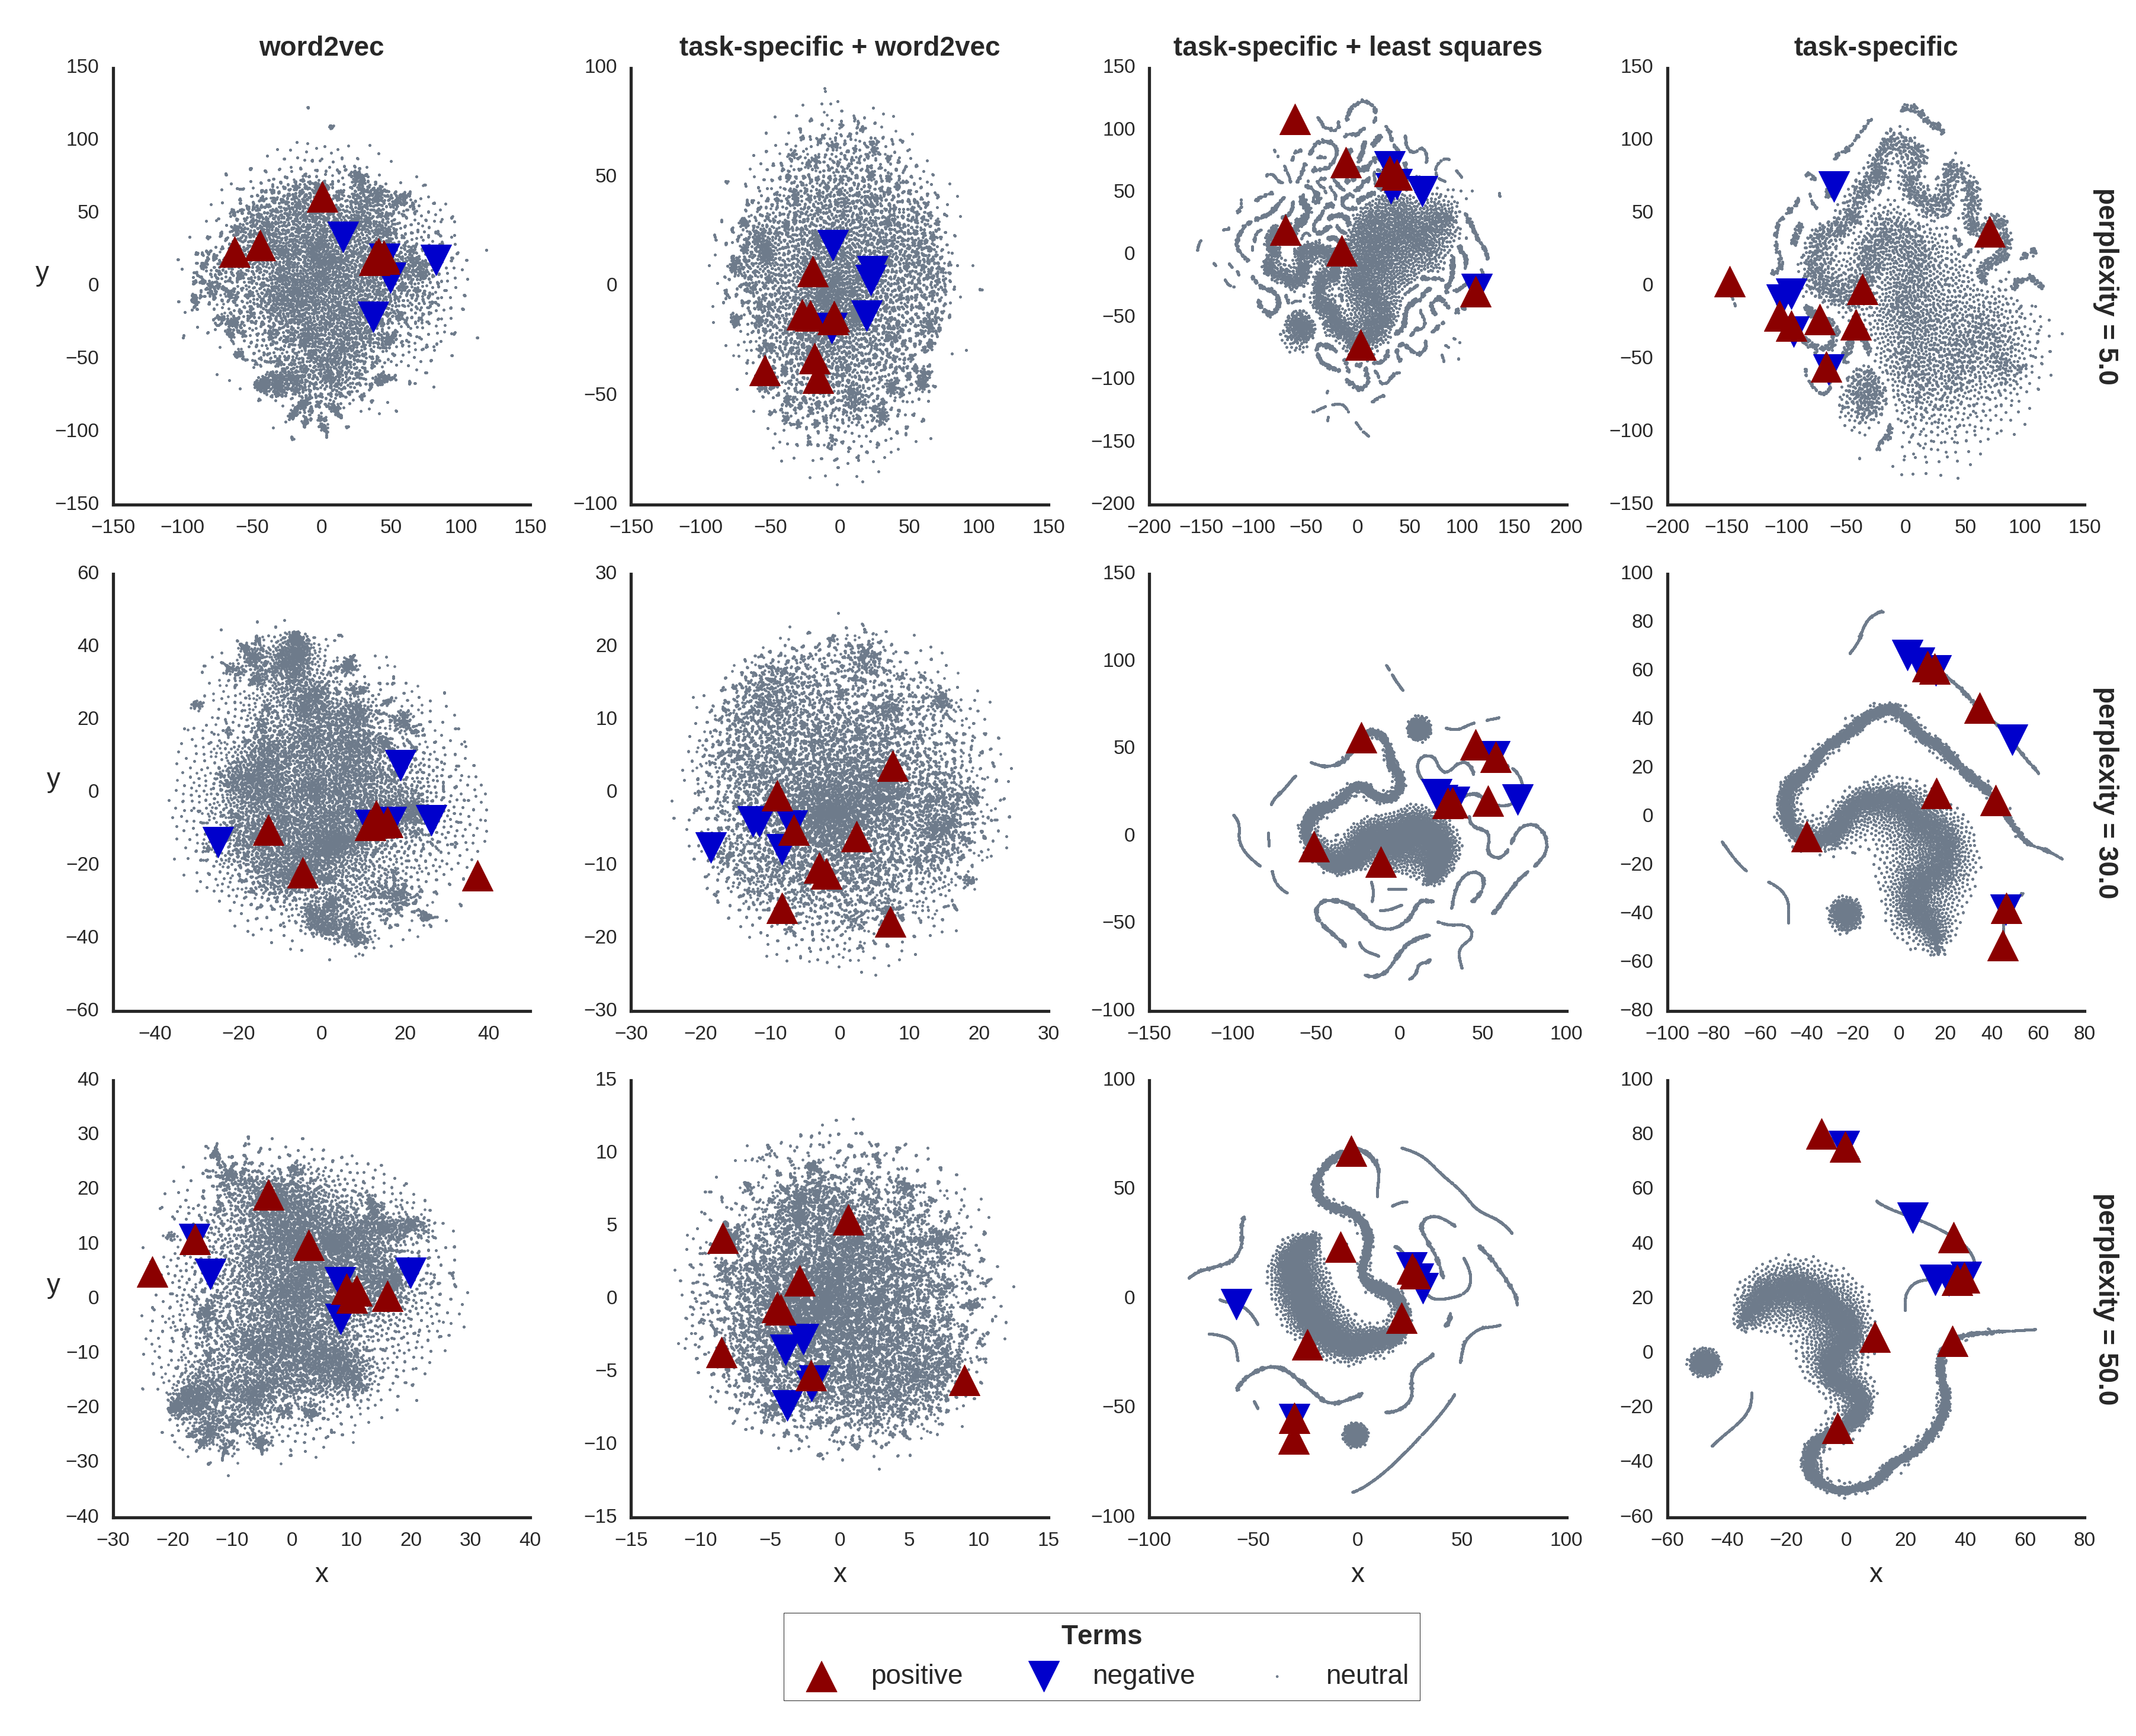
\includegraphics[height=30em,width=\linewidth]{img/potts_embeddings.png}
  \caption[Visualization of the \citeauthor{Turney:03}'s seed
    set]{t-SNE visualization of PotTS' tokens and
    \citeauthor{Turney:03}'s seed set with different embedding
    types}\label{snt:fig:tsne-seeds}
\end{figure}

\subsubsection{Vector Normalization}\label{subsec:snt-lex:eowet}

The final major factor which also could play a role in the quality of
NWE-induced polarity lists was the length normalization and mean
scaling, which we applied to word2vec vectors at the very beginning of
the training.

In the first stage of this preprocessing (during the length
normalization), we divided all embeddings by their Euclidean norm,
setting all of them to unit length:
\begin{align}
  E' &= \frac{E}{\norm{E}}.
\end{align}
Afterwards, we mean-normalized the resulting representations by
subtracting their means and dividing by the standard deviation:
\begin{align}
  E'' &= \frac{E' -\mu_{E'}}{\sigma_{E'}},
\end{align}
ensuring this way that the final coordinates of all embeddings were
centered around zero, and had a unit-variance in their distribution.

To check the effect of these procedures, we reran our NWE-based
algorithms without these normalization steps, and present the results
of our evaluation in Table~\ref{snt-lex:tbl:emb-evn}.  As we can see
from the scores, the method of the nearest centroids is almost
indifferent to the preprocessing, showing the same performance for all
settings.  However, the remaining three approaches ($k$-NN, PCA, and
the linear projection system) achieve their best results when both
normalization types are used.  Although we should admit that this
success is mostly due to the length normalization rather than mean
scaling.  We can recognize this by comparing the scores in the first
and third columns of the table where the PCA algorithm shows identical
results, and the scores of the $k$-NN and linear projection methods
differ by only 0.1\%.  We also can observe that the mean-scaling alone
has a strong negative effect on the linear projection system, pulling
its scores down by 3\% in comparison with the unnormalized vectors;
but at the same time it slightly improves the results of the $k$-NN
system, increasing them by 0.1\% as compared to the original
embeddings.

\begin{table}[thb!]
  \begin{center}
    \bgroup\setlength\tabcolsep{0.1\tabcolsep}%
    \setlength{\belowrulesep}{0pt}\scriptsize
    \begin{tabular}{p{0.145\columnwidth} % first columm
        *{4}{>{\centering\arraybackslash}p{0.21\columnwidth}}} % next four columns
      \toprule
      \multirow{2}*{\bfseries SLG Method} & \multicolumn{4}{c}{\bfseries Vector Normalization}\\
                                          & mean normalization + length normalization %
                                          & mean normalization %
                                          & length normalization %
                                          & no normalization\\\midrule
      NC & \textbf{0.398} & \textbf{0.398} & \textbf{0.398} & \textbf{0.398}\\
      $k$-NN & \textbf{0.468} & 0.418 & 0.467 & 0.417\\
      PCA & \textbf{0.398} & 0.396 & \textbf{0.398} & 0.396\\
      LP & \textbf{0.462} & 0.416 & 0.461 & 0.442\\\bottomrule

    \end{tabular}\egroup%
    {
      \captionsetup{justification=centering}
      \caption[Macro-averaged \F-scores of NWE-based methods with
        different vector normalizations]{Macro-averaged \F-scores of
        NWE-based methods with different vector
        normalizations}\label{snt-lex:tbl:emb-evn} }
  \end{center}
\end{table}

To visually demonstrate the effect of this preprocessing, we applied
these procedures to the two-dimensional sample vectors from
Section~\ref{subsec:snt:lex:nwe}, and present these results in
Figure~\ref{snt-lex:fig:nwe-norms}. As we can see from the picture,
the length normalization casts all embeddings on an $n$-dimensional
sphere, increasing the distance between the vectors with greater
mutual angles, but shortening the differences between those embeddings
whose in-between angles are small.  Vice versa, with the mean scaling,
the internal structure of the whole vector space is largely preserved
(up to a few outliers which become closer to the means), but their
general distribution becomes more condensed (which we can recognize
from the closer interval the embeddings appear in).  Finally, applying
both normalizations (first normalizing the length, and then the mean)
still makes the whole distribution spherical, but shifts the center of
this sphere towards the location of the majority of the points.

\begin{figure*}[hbt!]
  {
    \centering
    \begin{subfigure}{.5\textwidth}
      \centering
      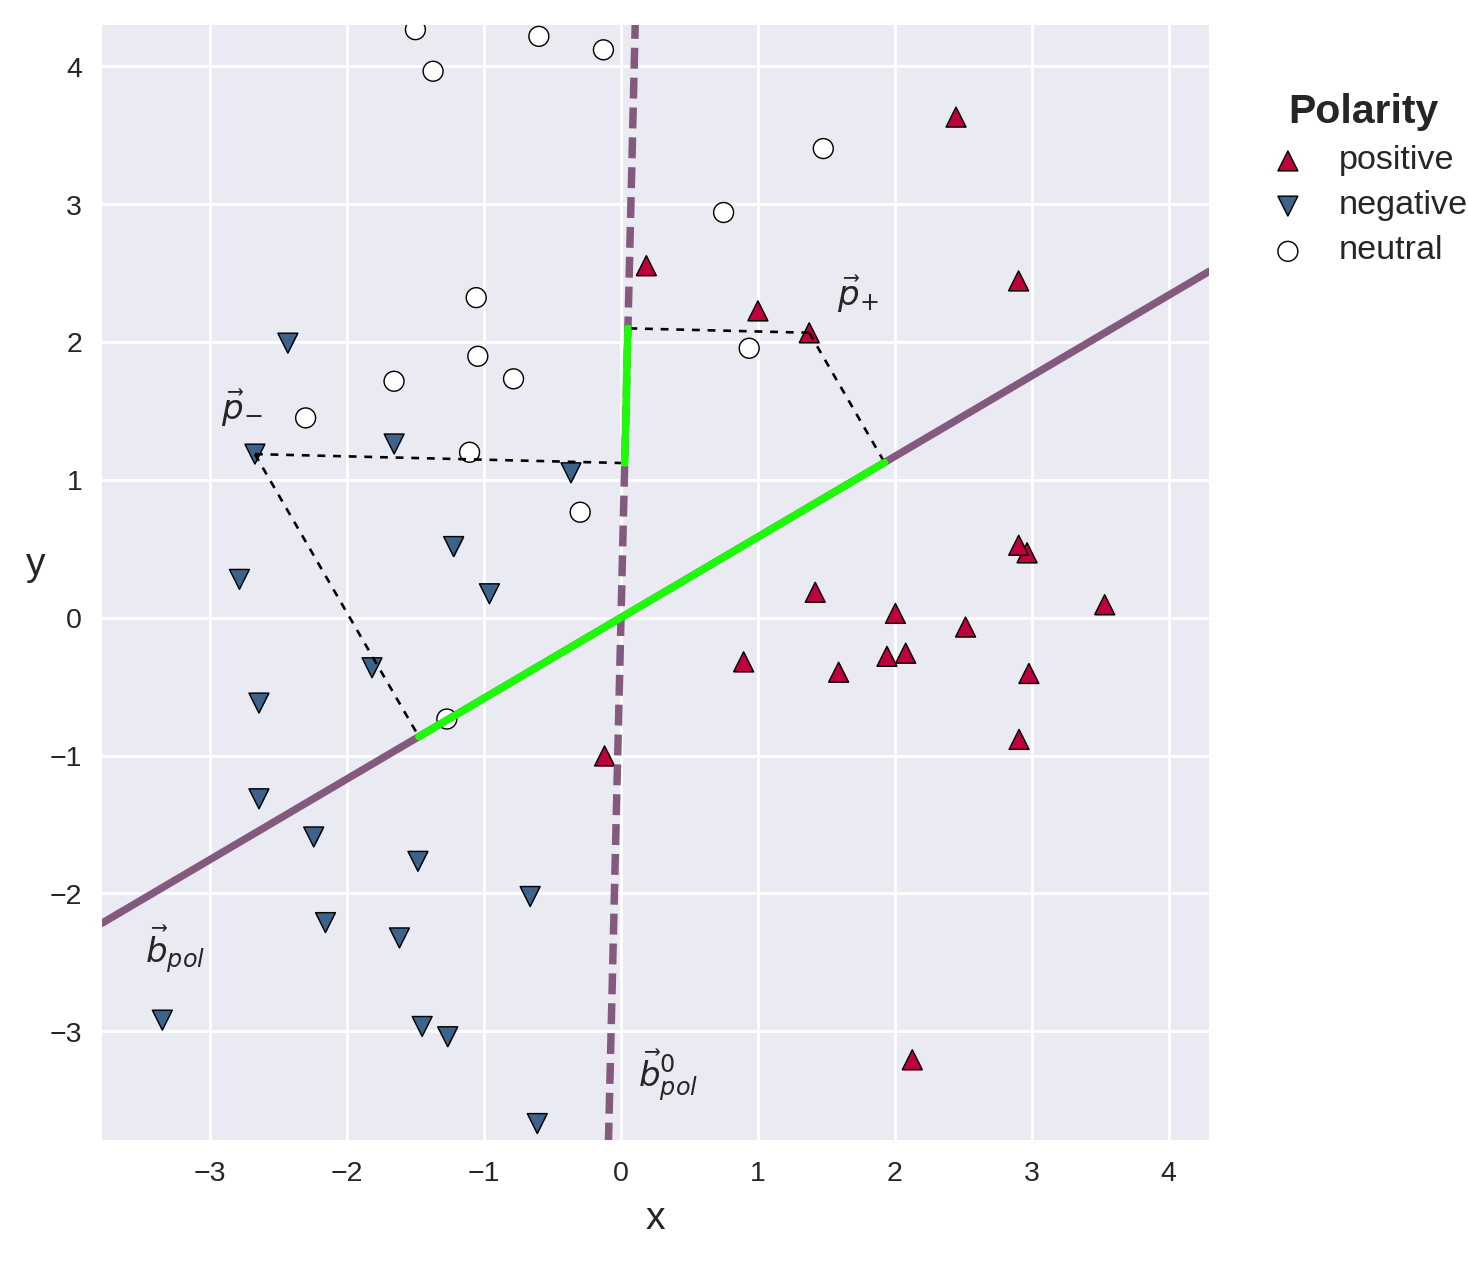
\includegraphics[width=\linewidth]{img/sentilex_polarity_not_normed.png}
      \caption{Without normalization}\label{snt-lex:fig:nwe-no-norm}
    \end{subfigure}%
    \begin{subfigure}{.5\textwidth}
      \centering
      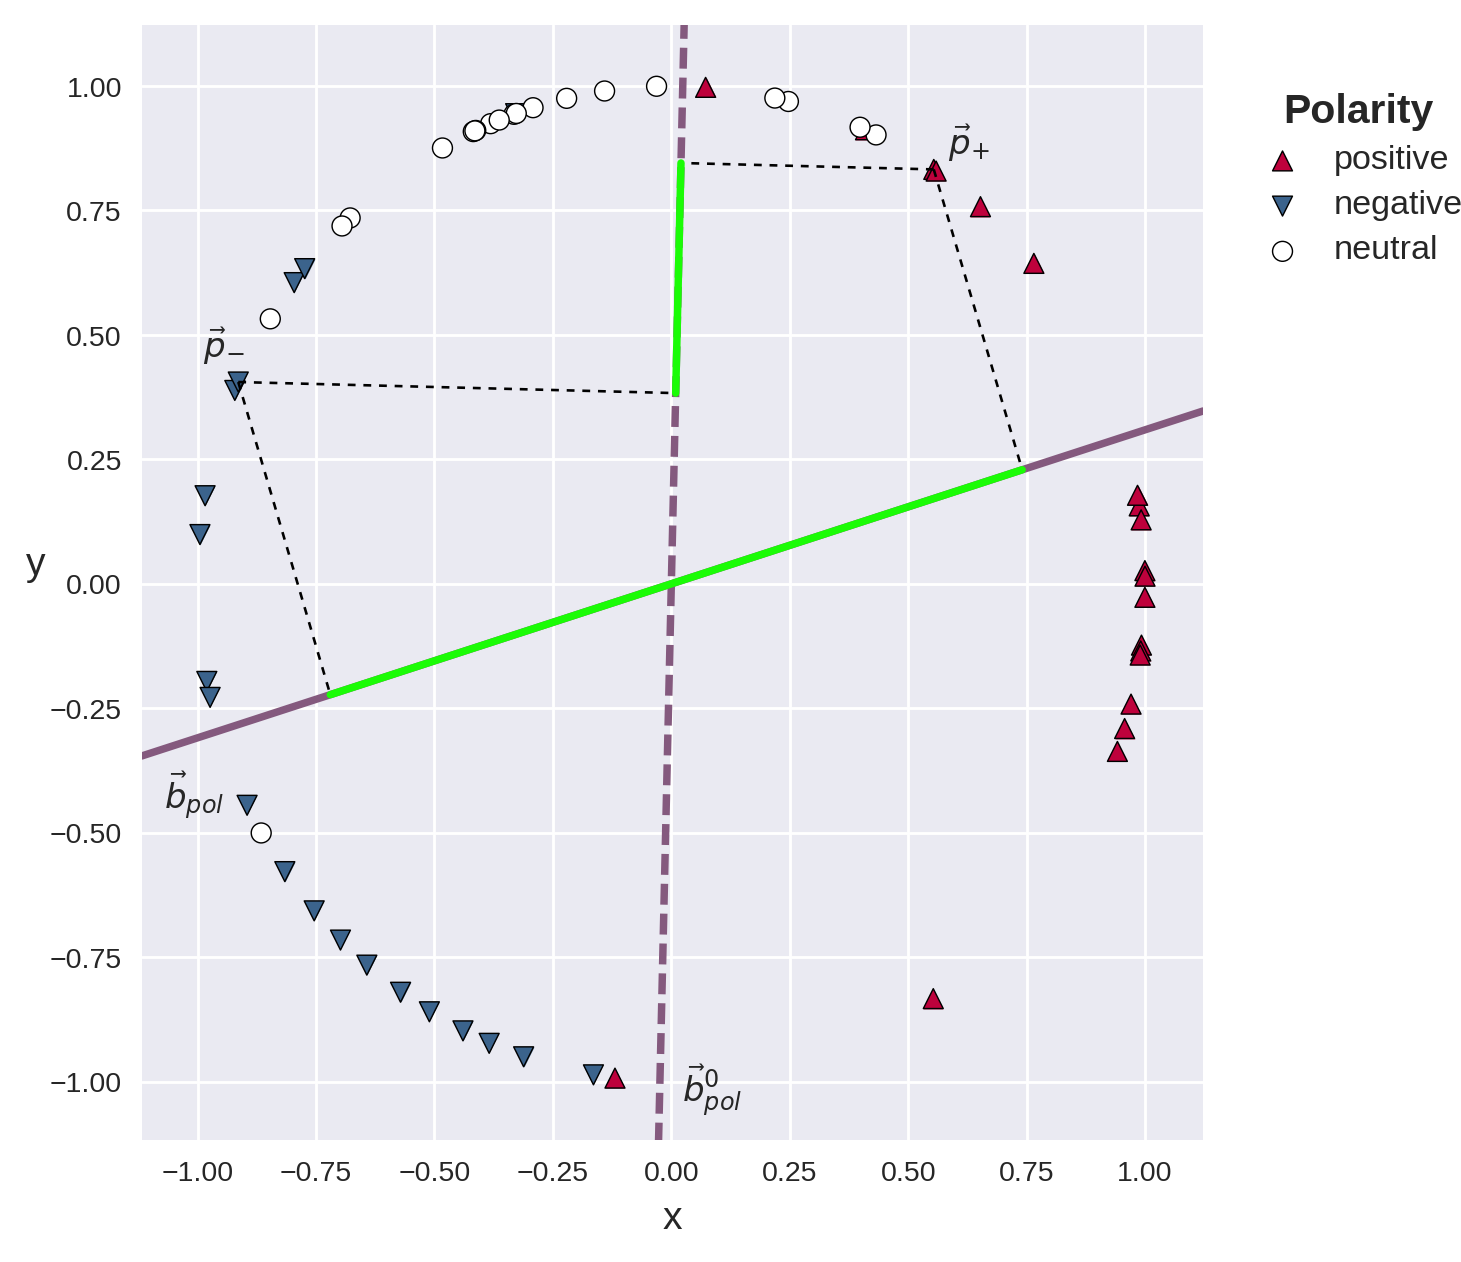
\includegraphics[width=\linewidth]{img/sentilex_polarity_len_normed.png}
      \caption{With length normalization}\label{snt-lex:fig:nwe-len-norm}
    \end{subfigure}\\
    \begin{subfigure}{.5\textwidth}
      \centering
      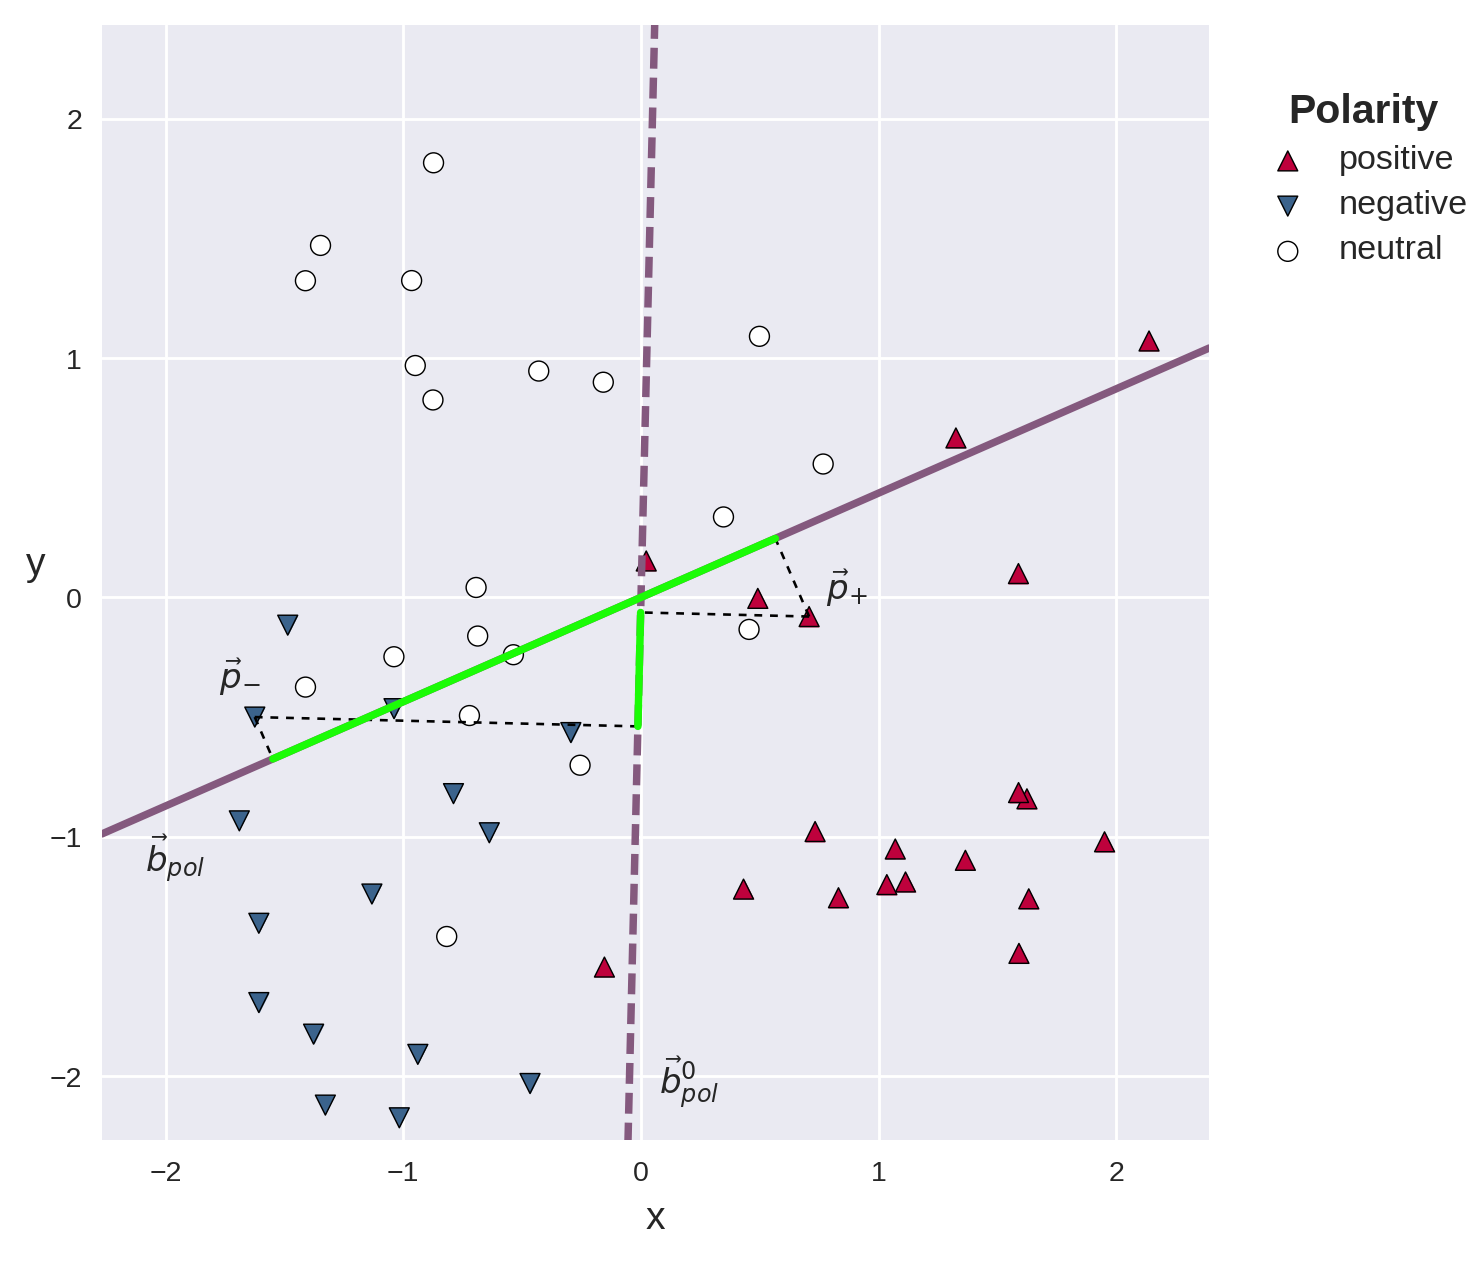
\includegraphics[width=\linewidth]{img/sentilex_polarity_mean_normed.png}
      \caption{With mean normalization}\label{snt-lex:fig:nwe-mean-norm}
    \end{subfigure}%
    \begin{subfigure}{.5\textwidth}
      \centering
      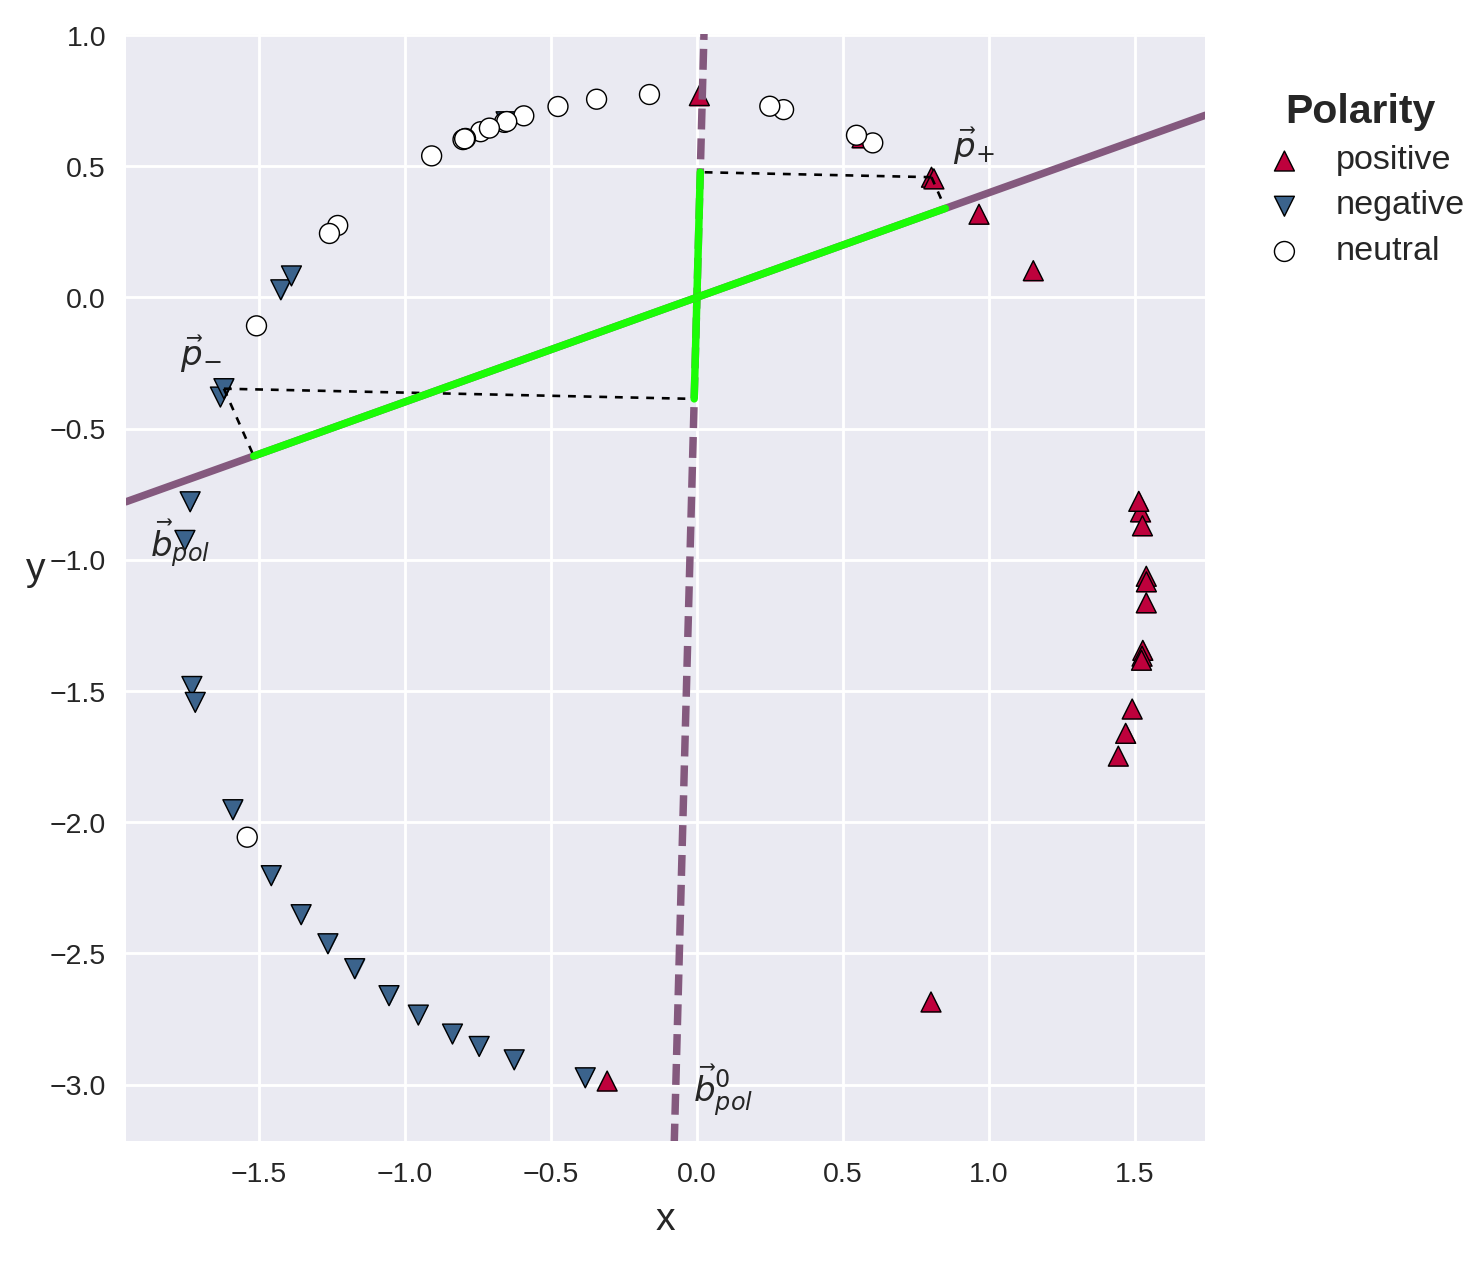
\includegraphics[width=\linewidth]{img/sentilex_polarity_len_mean_normed.png}
      \caption{With length and mean normalization}\label{snt-lex:fig:nwe-mean-len-mean-norm}
    \end{subfigure}
  }
  \caption{Polarity lines determined by the linear projection method
    with different vector normalizations}\label{snt-lex:fig:nwe-norms}
\end{figure*}

\section{Seed Sets}\label{subsec:snt-lex:eoss}

An important factor which could significantly affect the quality of
all resulting sentiment lexicons was the set of the seed terms that we
used to initialize the polarity scores of the tested methods.  In
order to estimate the impact of this setting on the final scores, we
re-run our experiments using the seed lists proposed by \citet{Hu:04},
\citet{Kim:04}, \citet{Esuli:06c}, and \citet{Remus:10}.  Since
\citet{Hu:04}, however, only partially specified their seed set in the
original paper, and \citet{Kim:04} did not provide any examples of
their seeds at all, we filled the missing entries in these resources
with common polar German words that we came up with in order to match
the reported sizes of these lists.  Furthermore, in the cases where
the above seed sets were missing the neutral category, we explicitly
added a number of objective terms proportional to the number of polar
entries in these lists.  Finally, as the number of neutral terms in
the polarity list of~\citet{Esuli:06c} run up to~4,122 words---the
authors considered as neutral all entries from the General Inquirer
lexicon \cite{Stone:66} which were not marked there as either positive
or negative and did not appear in the seed list of
\citet{Turney:03}---and were therefore tedious to translate manually,
we automatically obtained translations for these terms by using the
publicly available online dictionary
\texttt{dict.cc}\footnote{\url{http://www.dict.cc}} and taking the
first suggested German translation for each of the neutral
entries.\footnote{We also tried to use all possible translations of
  the original terms, but it lead to a considerable boost in the
  number of neutral items (45,252 words) and resulted in a substantial
  decrease of the final system scores.} A short statistics on the
cardinality and composition of the resulting seed lists is presented
in Table~\ref{snt-lex:tbl:alt-seed-sets}.

\begin{table}[h]
  \begin{center}
    \bgroup \setlength\tabcolsep{0.1\tabcolsep}\scriptsize
    \begin{tabular}{ %
        >{\centering\arraybackslash}p{0.2\columnwidth} % first columm
        >{\centering\arraybackslash}p{0.2\columnwidth} % next column
        >{\centering\arraybackslash}p{0.1\columnwidth} % next column
        *{2}{>{\centering\arraybackslash}p{0.243\columnwidth}}} % final two columns
      \toprule
      {\bfseries Seed Set} & %
      {\bfseries Cardinality} & %
      {\bfseries Part of Speech} & %
      {\bfseries Examples} & %
      {\bfseries Comments}\\
      \midrule
      \citet{Hu:04} & 14 positive, 15 negative, and 10 neutral terms & adjectives %
      & {{\itshape fantastisch, lieb, sympathisch, %
          b\"ose, dumm, schwierig}} & polar terms translated from the original paper %
      \cite{Hu:04}; neutral terms added by us;\\
      \citet{Kim:04} & 60 positive, 60 negative, and 60 neutral terms & any & %
      {\itshape fabelhaft, Hoffnung, lieben, h\"asslich, Missbrauch, t\"oten} %
      & devised by us to match the cardinality of the original set with %
      neutral terms added extra;\\
      \citet{Esuli:06c} & 16 positive, 35 negative, and 4,122 neutral terms & %
      any & {\itshape angenehm, ausgezeichnet, freundlich, %
        arm, bedauernswert, d\"urftig} & polar terms translated from the seed %
      set of \citet{Turney:03}; neutral terms automatically translated from %
      objective entries in the General Inquirer lexicon \cite{Stone:66};\\
      \citet{Remus:10} & 12 positive, 12 negative, and 10 neutral terms & %
      adjectives & {\itshape gut, sch\"on, richtig, %
        schlecht, unsch\"on, falsch} & %
      polar terms translated from the seed set of \citet{Turney:03}; %
      neutral terms added by us;\\
      \\\bottomrule
    \end{tabular}
    \egroup
    \caption[Overview of alternative seed sets]{ Overview of
      alternative seed sets\\ (all cardinalities are given with
      respect to the resulting German translations)}
    \label{snt-lex:tbl:alt-seed-sets}
  \end{center}
\end{table}

The updated results of the dictionary-based approaches with these
alternative seed sets are shown in
Figure~\ref{snt:fig:sent-dict-lex-alt-seeds}.  This time, we again can
notice the superior scores achieved by the method of
\citet{Blair-Goldensohn:08}, which not only outperforms other systems
on average, but also seems to be less susceptible to the varying
quality and size of different seeds.  The remaining methods typically
achieve their best macro-averaged \F{}-results with either of the two
top-performing initial polarity lists: the one of \citet{Kim:04} or
the one proposed by~\citet{Esuli:06c}.  The former option works best
for the label-propagation approach of \citet{Rao:09} and the random
walk algorithm of \citet{Awadallah:10}.  Moreover, the results shown
by the min-cut system of~\citet{Rao:09} and the original method of
\citet{Kim:04} in combination with these seeds are only slightly lower
than their respective scores achieved with the best possible
configuration---the seed list of \citet{Turney:02}.  The latter
option---the seed set of~\citet{Esuli:06c}---yields best results for
the approaches of~\citet{Hu:04} and the \textsc{SentiWordNet} method
of~\citet{Esuli:06c}.

\begin{figure}[hbtp]
  \centering
  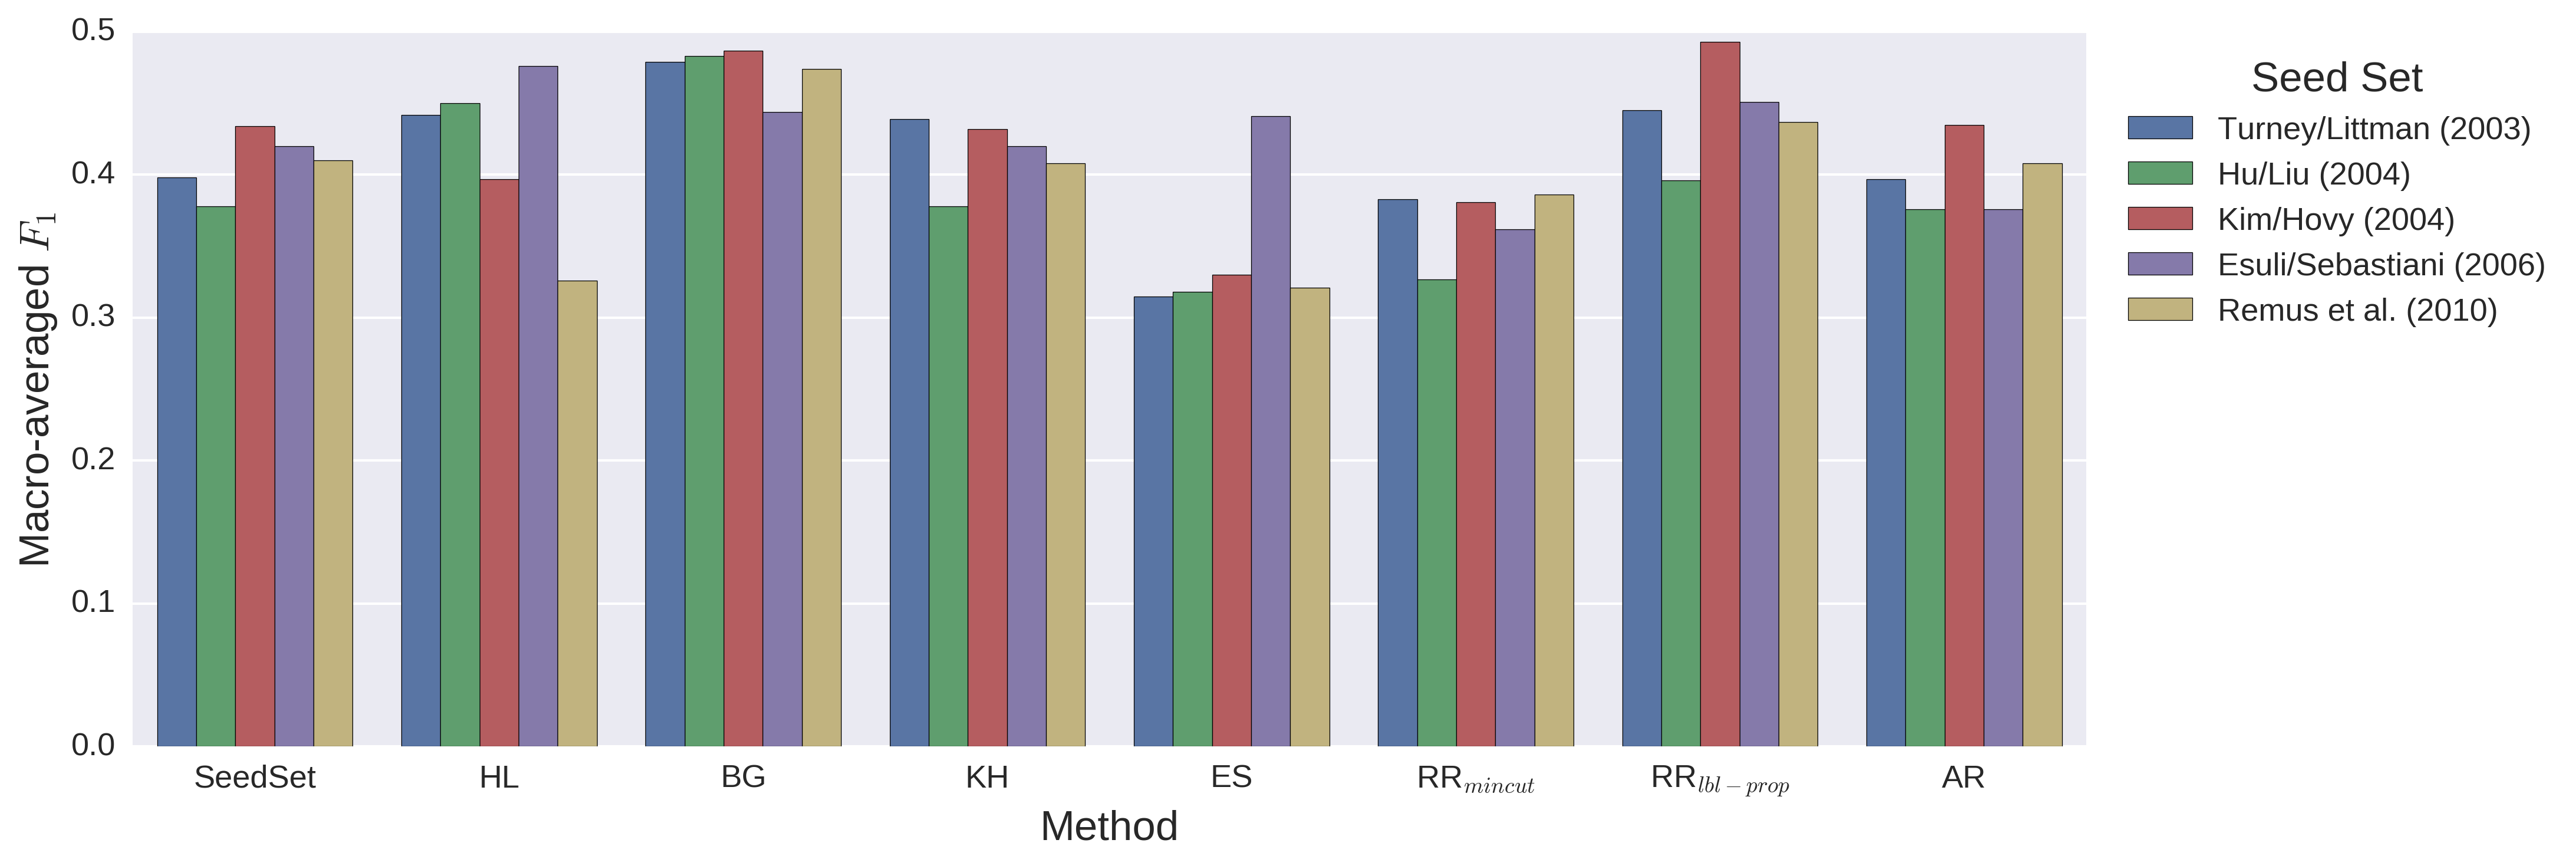
\includegraphics[height=12em,width=\linewidth]{%
    img/sentilex-dict-alt-seed-sets.png}
  \caption{Macro-averaged \F{}-scores of dictionary-based approaches
    with different seed sets}\label{snt:fig:sent-dict-lex-alt-seeds}
\end{figure}

A somewhat different situation is observed for the corpus-based
approaches as shown in Figure~\ref{snt:fig:sent-crp-lex-alt-seeds}.
Except for the method of \citet{Takamura:05}, which achieves its best
result with the seed set of \citet{Hu:04}, all three remaining
methods---\citet{Velikovich:10}, \citet{Kiritchenko:14}, and
\citet{Severyn:15}---show very similar (though not identical) scores
to the ones reached by the non-expanded seed sets.  The primary reason
for this is again the ambiguity of the translated seeds, which causes
a rapid decrease of the lexicon quality and, consequently, an early
stopping of the expansion.

As to the NWE-based methods, whose scores are presented in
Figure~\ref{snt:fig:sent-nwe-lex-alt-seeds}, we anew can notice the
impressive performance of the $k$-NN and linear projection systems.
This time, however, we also can see a complementary behavior of these
two approaches on different seed lists: the $k$-NN algorithm attains
better results with the seed set of~\citet{Turney:03} than with the
seeds proposed by~\citet{Hu:04}, and it also gets higher scores with
the initial polar terms of~\citet{Remus:10} than with the ones
suggested by~\citet{Esuli:05}.  An opposite situation is observed for
the linear projection method, which achieves a macro-average of~0.478
with the seed set of~\citet{Hu:04} versus 0.462 macro-\F{} scored with
the seeds of~\citet{Turney:03}, and also shows better scores with the
seed list of~\citet{Esuli:05}~(0.456) than with the terms proposed
by~\citet{Remus:10}~(0.449).  A common feature of both of these
methods, however, is that they both obtain their best results with the
seed set of~\citet{Kim:04}, with which the $k$-NN approach attains a
macro-average of~0.508, and the linear projection algorithm reaches a
remarkable \F-score of~0.513 points, surpassing all other automatic
SLG method and establishing a new state-of-the-art landmark on this
metric.

\begin{figure}[hbtp]
  \centering
  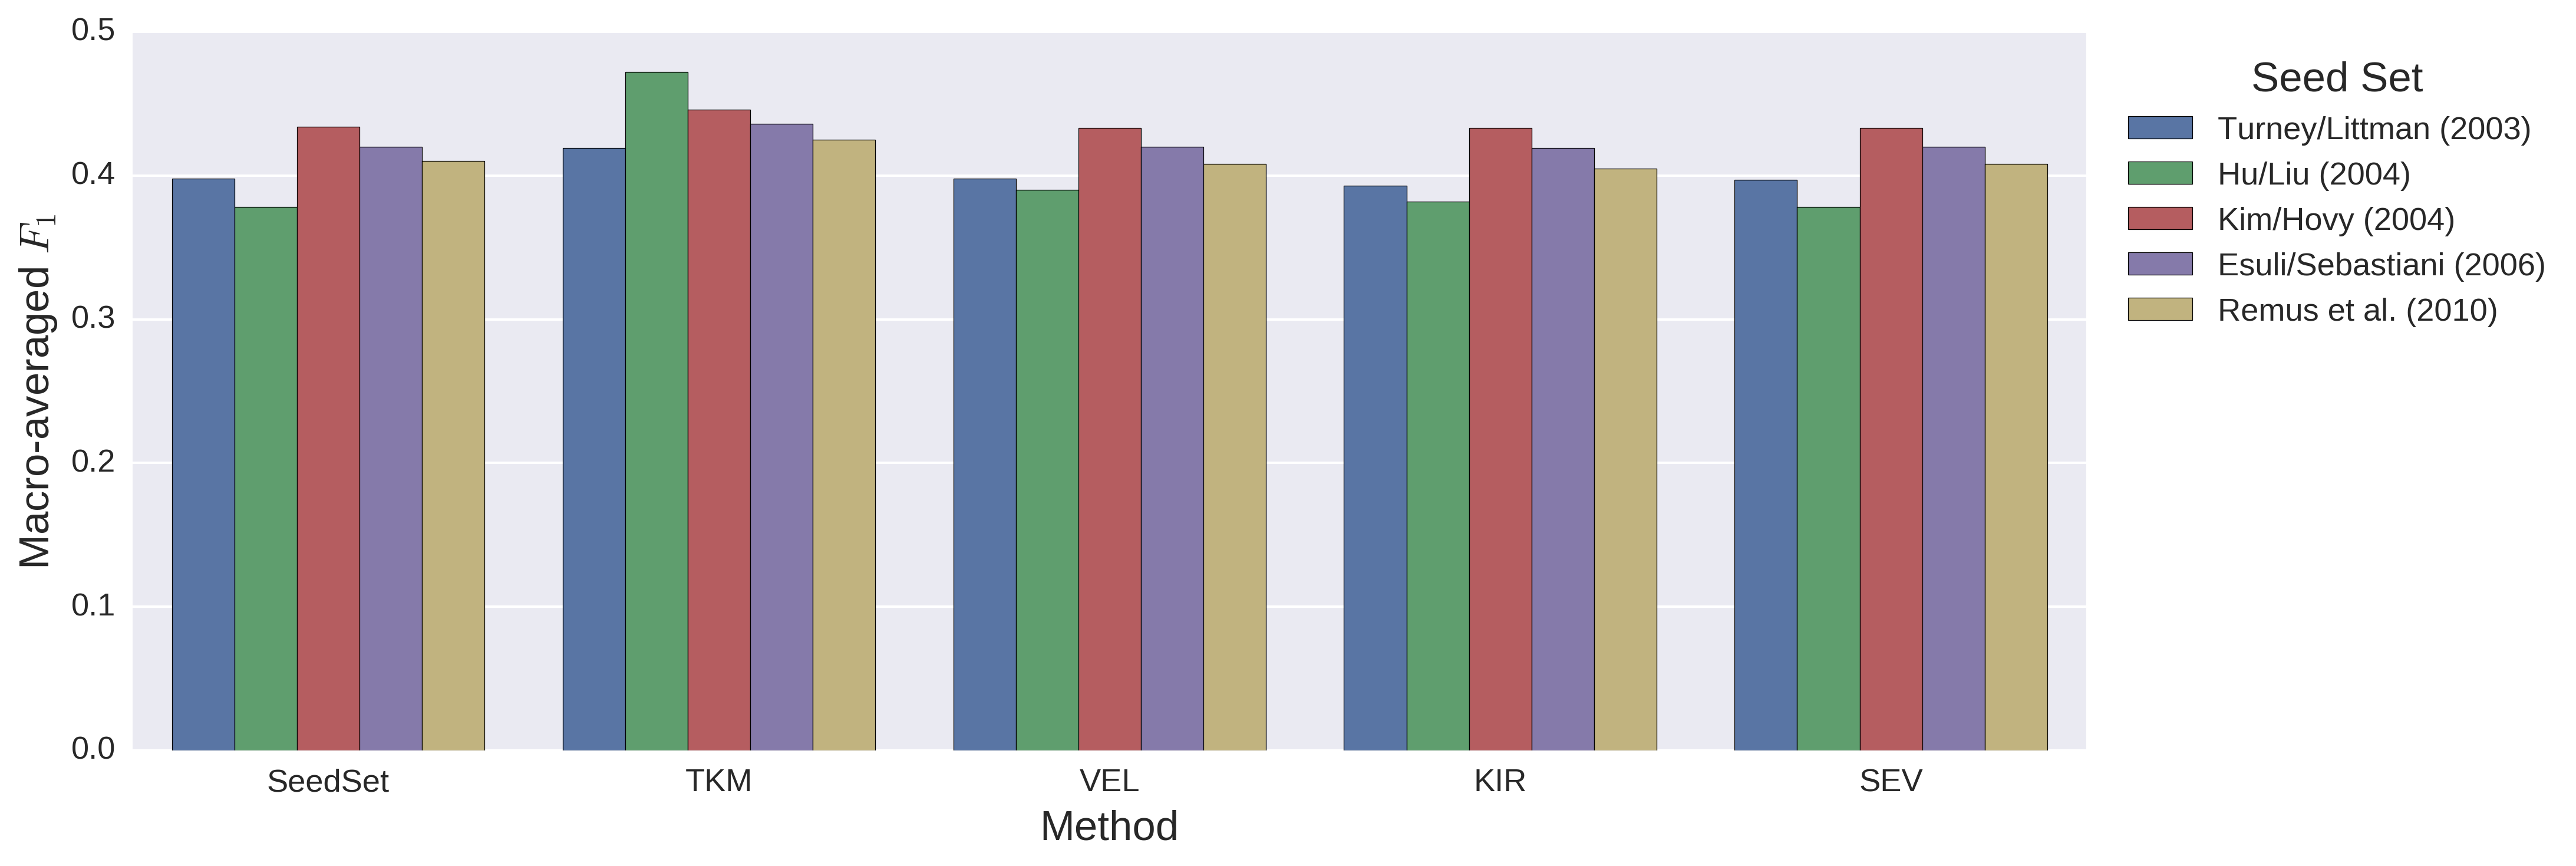
\includegraphics[height=12em,width=\linewidth]{%
    img/sentilex-crp-alt-seed-sets.png}
  \caption{Macro-averaged \F{}-scores of corpus-based approaches with
    different seed sets}\label{snt:fig:sent-crp-lex-alt-seeds}
\end{figure}

% In conformity with the results in Table~\ref{snt-lex:tbl:nwe-meth},
% the third-best macro-averaged results with the most common seed
% sets---the ones suggested by~\citet{Turney:03}, \citet{Hu:04}, and
% \citet{Kim:04}---were attained with the method of~\citet{Tang:16}.
% This approach, however, yielded significantly worse scores when used
% with the seed lists of~\citet{Esuli:05} and \citet{Remus:10}.

\begin{figure}[hbtp]
  \centering
  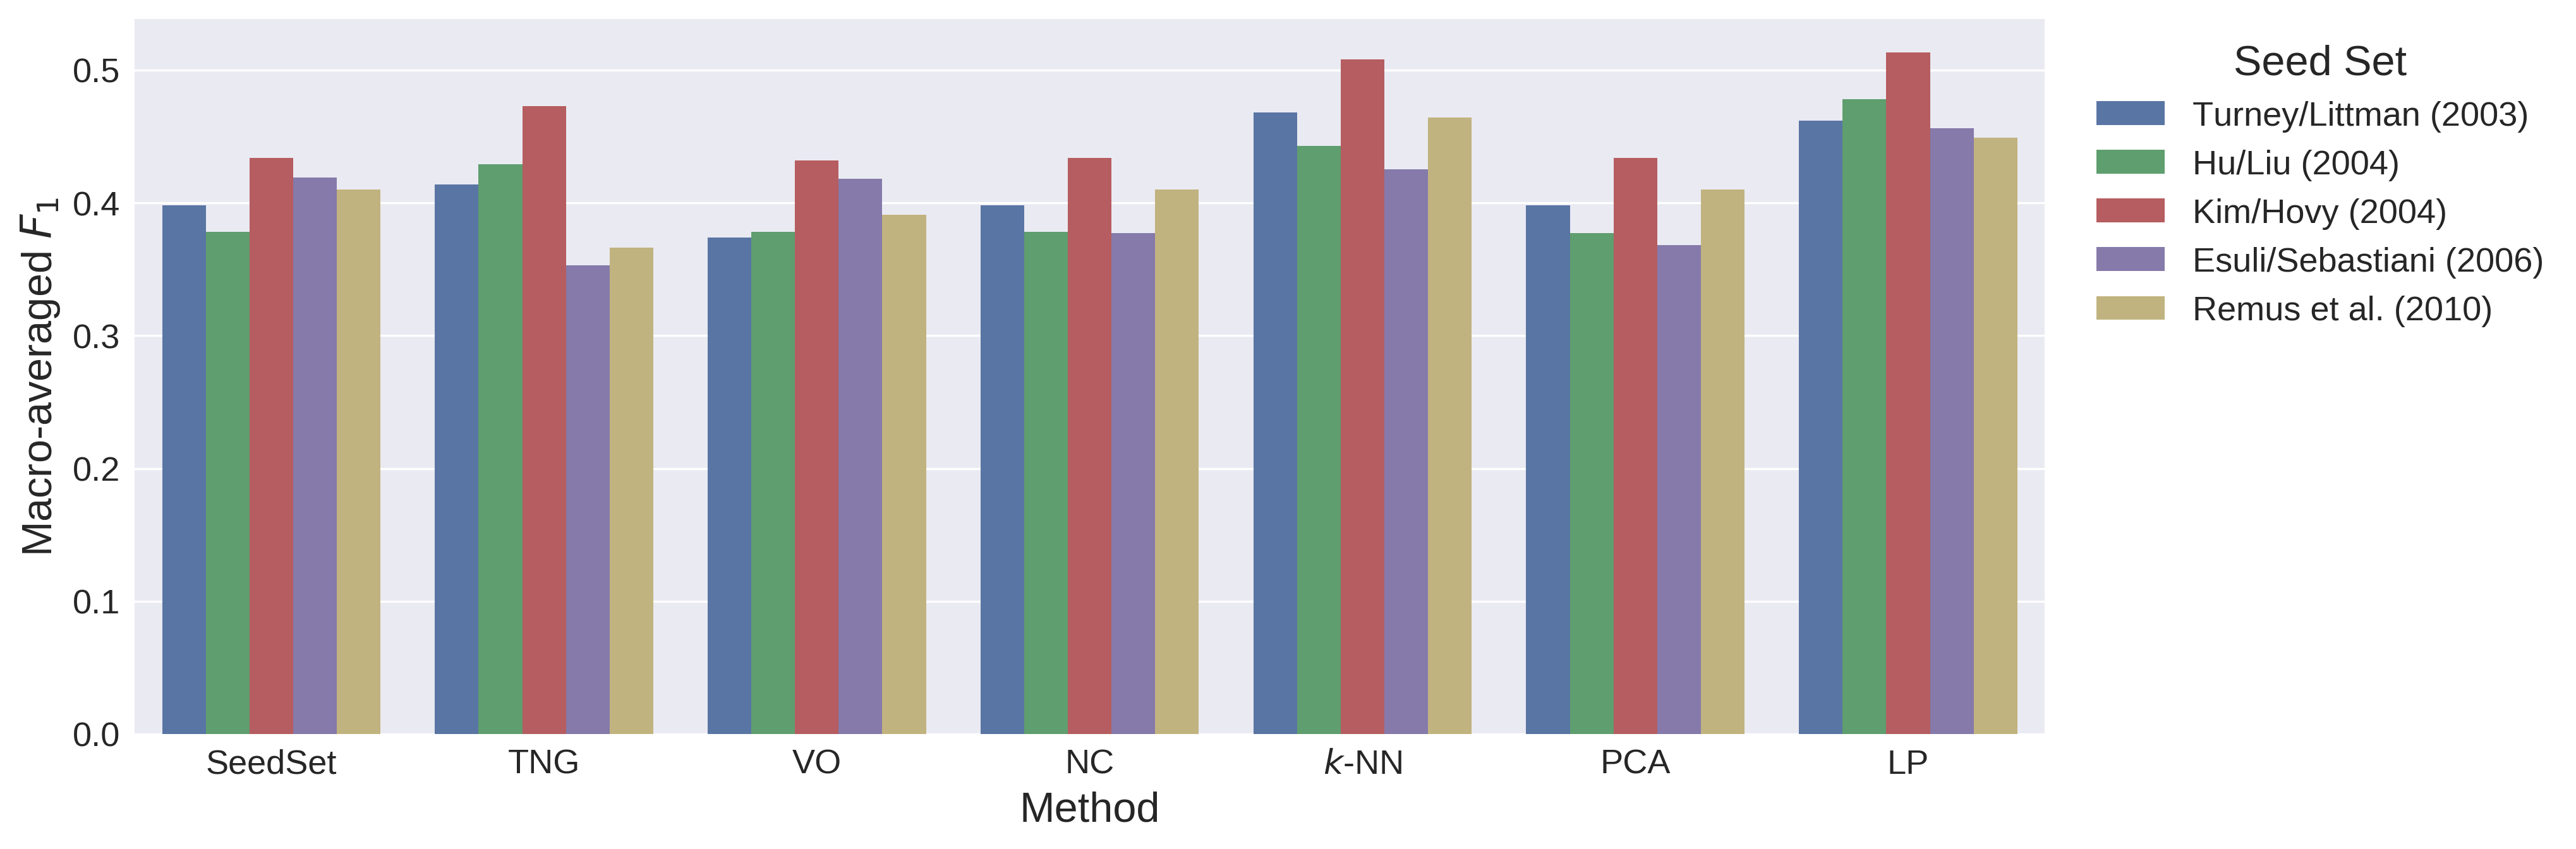
\includegraphics[height=12em,width=\linewidth]{%
    img/sentilex-nwe-alt-seed-sets.png}
  \caption{Macro-averaged \F{}-scores of NWE-based approaches with
    different seed sets}\label{snt:fig:sent-nwe-lex-alt-seeds}
\end{figure}

The remaining NWE-based systems also achieve their best results with
the seed set of~\citet{Kim:04}, which is not surprising considering
the much bigger size of this list.  Furthermore, the approaches of the
nearest centroids, principal components, and the distantly supervised
method of~\citet{Vo:16} show almost identical scores on all other seed
collections.

\section{Analysis of Entries}\label{subsec:snt-lex:aoe}

Besides investigating the effects of different hyper-parameters and
seed sets, we also decided to have a closer look at the actual results
produced by the tested methods.  For this purpose, we extracted ten
highest scored entries (not counting the seed terms) from each
dictionary-based automatic lexicon and summarized them in
Table~\ref{tbl:snt-lex:dict:top-10}.

\begin{table}[h]
  \begin{center}
    \bgroup \setlength\tabcolsep{0.03\tabcolsep}\scriptsize
    \begin{tabular}{%
        >{\centering\arraybackslash}p{0.065\columnwidth} % first columm
        *{6}{>{\centering\arraybackslash}p{0.155\columnwidth}}} % last two columns
      \toprule
      \textbf{Rank} & %
      \textbf{HL} & \textbf{BG} & \textbf{KH} & %
      \textbf{ES} & \textbf{RR}$^{**}_{\textrm{mincut}}$ & %
      \textbf{RR}$_{\textrm{lbl-prop}}$\\\midrule
      1 & \ttranslate{perfekt}{perfect} & %
      \ttranslate{flei\ss{}ig}{diligent} &%
      \ttranslate{anr\"uchig}{indecent} &%
      \ttranslate{namenlos}{nameless} &%
      \ttranslate{planieren}{to plane} &%
      \ttranslate{prunkvoll}{splendid}\\

      2 & \ttranslate{musterg\"ultig}{immaculate} & %
      \ttranslate{b\"ose}{evil} &%
      \ttranslate{unecht}{artificial} &%
      \ttranslate{ruhelos}{restless} &%
      \ttranslate{Erdschicht}{stratum} &%
      \ttranslate{sinnlich}{sensual}\\


      3 & \ttranslate{vorbildlich}{commendable} & %
      \ttranslate{beispielhaft}{exemplary} &%
      \ttranslate{irregul\"ar}{irregular} &%
      \ttranslate{unbewaffnet}{unarmed} &%
      \ttranslate{gefallen}{please} &%
      \ttranslate{pomp\"os}{ostentatious}\\

      4 & \ttranslate{beispielhaft}{exemplary} & %
      \ttranslate{edel}{noble} &%
      \ttranslate{drittklassig}{third-class} &%
      \ttranslate{interesselos}{indifferent} &%
      \ttranslate{Zeiteinheit}{time unit} &%
      \ttranslate{unappetitlich}{unsavory}\\

      5 & \ttranslate{exzellent}{excellent} & %
      \ttranslate{t\"uchtig}{proficient} &%
      \ttranslate{sinnlich}{sensual} &%
      \ttranslate{reizlos}{unattractive} &%
      \ttranslate{Derivat}{derivate} &%
      \ttranslate{befehlsgem\"a\ss{}}{as ordered}\\

      6 & \ttranslate{exzeptionell}{exceptional} & %
      \ttranslate{emsig}{busy} &%
      \ttranslate{unprofessionell}{unprofessional} &%
      \ttranslate{w\"urdelos}{undignified} &%
      \ttranslate{Oberfl\"ache}{surface} &%
      \ttranslate{vierschr\"otig}{beefy}\\

      7 & \ttranslate{au\ss{}ergew\"ohnlich}{extraordinary} & %
      \ttranslate{eifrig}{eager} &%
      \ttranslate{abgeschlagen}{exhausted} &%
      \ttranslate{absichtslos}{unintentional} &%
      \ttranslate{Essbesteck}{cutlery} &%
      \ttranslate{regelgem\"a\ss}{regularly}\\

      8 & \ttranslate{au\ss{}erordentlich}{exceptionally} & %
      \ttranslate{arbeitsam}{hardworking} &%
      \ttranslate{gef\"allig}{pleasing} &%
      \ttranslate{ereignislos}{uneventful} &%
      \ttranslate{abl\"osen}{to displace} &%
      \ttranslate{wahrheitsgem\"a\ss}{true}\\

      9 & \ttranslate{viertklassig}{fourth-class} & %
      \ttranslate{musterg\"ultig}{exemplary} &%
      \ttranslate{musterg\"ultig}{exemplary} &%
      \ttranslate{regellos}{irregular} &%
      \ttranslate{Musikveranstaltung}{music event} &%
      \ttranslate{fettig}{greasy}\\

      10 & \ttranslate{sinnreich}{ingenious} & %
      \ttranslate{vorbildlich}{commendable} &%
      \ttranslate{unrecht}{wrong} &%
      \ttranslate{fehlerfrei}{accurate} &%
      \ttranslate{Gebrechen}{afflictions} &%
      \ttranslate{lumpig}{shabby}\\\bottomrule
    \end{tabular}
    \egroup
    \caption[Top ten polar terms produced by dictionary-based
    methods]{%
      Top ten polar terms produced by dictionary-based methods\\
      {\small ** -- the min-cut method of \citet{Rao:09} returns an
        unsorted set}}
    \label{tbl:snt-lex:dict:top-10}
  \end{center}
\end{table}

As can be seen from the table, the approaches of \citet{Hu:04},
\citet{Blair-Goldensohn:08}, \citet{Kim:04}, as well as the
label-propagation algorithm of \citet{Rao:09} produce almost perfect
polarity lists.  The \textsc{SentiWordNet} approach of
\citet{Esuli:06c}, however, already features some spurious terms among
its top-scored entries (e.g., ``absichtslos'' \emph{unintentional}).
Finally, the min-cut approach of \citet{Rao:09} returns a set of
mainly objective terms, which, however, is rather due to the fact that
this method performs a cluster-like partitioning of the lexical graph
without actually ranking the words assigned to a cluster.

A different situation is observed with the corpus-based systems as
shown in Table~\ref{tbl:snt-lex:crp:top-10}: The top-scoring polarity
lists returned by all of these approaches not only include many
apparently objective terms, but are also difficult to interpret in
general, as they contain a substantial number of slang and advertising
expressions (e.g., ``BMKS65,'' ``\#gameinsight,'' ``\#androidgames'').

\begin{table}[hbt!]
  \begin{center}
    \bgroup \setlength\tabcolsep{0.03\tabcolsep}\scriptsize
    \begin{tabular}{%
        >{\centering\arraybackslash}p{0.06\columnwidth} % first columm
        *{4}{>{\centering\arraybackslash}p{0.233\columnwidth}}} % last two columns
      \toprule
      \textbf{Rank} & %
      \textbf{TKM} & \textbf{VEL} & \textbf{KIR} & %
      \textbf{SEV} \\\midrule
      1 & \ttranslate{Stockfotos}{stock photos} &%
      \ttranslate{Wahl\-kampf\-ge\-schenk}{election gift} &%
      \ttranslate{Suchmaschinen}{search engines} &%
      \ttranslate{Scherwey}{Scherwey}\\

      2 & \ttranslate{BMKS65}{BMKS65} &%
      \ttranslate{Or\-dens\-ge\-schich\-te}{order history} &%
      \ttranslate{\#gameinsight}{\#gameinsight} &%
      \ttranslate{krebsen}{to crawl}\\

      3 & \ttranslate{Ziya}{Ziya} &%
      \ttranslate{Indologica}{Indologica} &%
      \ttranslate{\#androidgames}{\#androidgames} &%
      \ttranslate{kaschieren}{to conceal}\\

      4 & \ttranslate{Shoafoundation}{shoah found.} &%
      \ttranslate{Indologie}{Indology} &%
      \ttranslate{Selamat}{selamat} &%
      \ttranslate{Davis}{Davis}\\

      5 & \ttranslate{T1199}{T1199} &%
      \ttranslate{Energieverbrauch}{energy consumption} &%
      \ttranslate{Pagi}{Pagi} &%
      \ttranslate{\#Klassiker}{\#classics}\\

      6 & \ttranslate{Emilay55}{Emilay55} &%
      \ttranslate{Schimmelbildung}{mold formation} &%
      \ttranslate{\#Sparwelt}{\#savingsworld} &%
      \ttranslate{Nationalismus}{nationalism}\\

      7 & \ttranslate{Eneramo}{Eneramo} &%
      \ttranslate{Hygiene}{hygiene} &%
      \ttranslate{\#Seittest}{\#Seittest} &%
      \ttranslate{Kraftstoff}{fuel}\\

      8 & \ttranslate{GotzeID}{GotzeID} &%
      \ttranslate{wasserd}{waterp} &%
      \ttranslate{Gameinsight}{Gameinsight} &%
      \ttranslate{inaktiv}{idle}\\

      9 & \ttranslate{BSH65}{BSH65} &%
      \ttranslate{heizkostensparen}{saving heating costs} &%
      \ttranslate{\#ipadgames}{\#ipadgames} &%
      \ttranslate{8DD}{8DD}\\

      10 & \ttranslate{Saymak.}{Saymak.} &%
      \ttranslate{Re\-fe\-renz\-ar\-chi\-tek\-tu\-ren}{reference architectures} &%
      \ttranslate{Fitnesstraining}{fitness training} &%
      \ttranslate{Mailadresse}{mail address}\\\bottomrule
    \end{tabular}
    \egroup
    \caption[Top ten polar terms produced by corpus-based
    methods]{Top ten polar terms produced by corpus-based methods}
    \label{tbl:snt-lex:crp:top-10}
  \end{center}
\end{table}

We can also observe a similar trend for the most NWE-based methods,
whose results are presented in Table~\ref{tbl:snt-lex:NWE:top-10}.  As
we can see from the examples, many of these systems obviously overrate
Internet-specific terms (e.g., ``\%user-playlist'', ``\%user-video'',
``www.op''), and assign higher weights to foreign words (e.g.,
``nerelere'', ``good'', ``nativepride'') and interjections (e.g.,
``niedlichg\"ahn'' \emph{cuteyawn}, ``vrrrum'').  Two notable
exceptions from this trend are the {$k$-NN} and linear projection
systems, whose top-scoring entries contain exclusively polar terms,
supporting the promising findings in our foregoing evaluation.  At the
same time, we also can notice a slight susceptibility of these
approaches to the negative polarity class as eight out of ten highest
ranked words in their results have negative semantic orientation.  One
possible explanation for this could be a more pronounced distribution
of negative expressions, which pushes the vectors of these terms to
more distinguishable regions than in the case of positive lexemes.

\begin{table}[hbt!]
  \begin{center}
    \bgroup \setlength\tabcolsep{0.03\tabcolsep}\scriptsize
    \begin{tabular}{%
        >{\centering\arraybackslash}p{0.07\columnwidth} % first columm
        *{6}{>{\centering\arraybackslash}p{0.154\columnwidth}}} % last two columns
      \toprule
      \textbf{Rank} %
      & \textbf{TNG} & \textbf{VO} & \textbf{NC} %
      & \textbf{$k$-NN} & \textbf{PCA} & \textbf{LinProj} \\\midrule

      1 & \ttranslate{internetvorr\"ate}{Internet inventories} &%
      \ttranslate{guz}{guz} &%
      \ttranslate{paion}{paion} &%
      \ttranslate{eklig}{yukky} &%
      \ttranslate{gwiyomi.}{gwiyomi.} &%
      \ttranslate{dumm}{stupid}\\

      2 & \ttranslate{\%user-playlist}{\%user playlist} &%
      \ttranslate{nerelere}{nerelere} &%
      \ttranslate{auf$\lrcorner$}{on$\lrcorner$} &%
      \ttranslate{\"atzend}{lousy} &%
      \ttranslate{seitens}{on the part of} &%
      \ttranslate{eklig}{yukky}\\

      3 & \ttranslate{dumm}{stupid} &%
      \ttranslate{www.op}{www.op} &%
      \ttranslate{folgen!}{follow!} &%
      \ttranslate{l\"acherlich}{ridiculous} &%
      \ttranslate{kritisieren}{to criticize} &%
      \ttranslate{fies}{nasty}\\

      4 & \ttranslate{wundersch\"on}{gorgeous} &%
      \ttranslate{fernsehfestival}{TV festival} &%
      \ttranslate{teil8}{part8} &%
      \ttranslate{doof}{dumb} &%
      \ttranslate{nanda}{nanda} &%
      \ttranslate{doof}{dumb}\\

      5 & \ttranslate{\"olgem\"alde}{oil painting} &%
      \ttranslate{positip}{positip} &%
      \ttranslate{stanzmesser}{punch knife} &%
      \ttranslate{dumm}{stupid} &%
      \ttranslate{@deinskysport}{@deinskysport} &%
      \ttranslate{bl\"od}{stupid}\\

      6 & \ttranslate{\%user-video}{\%user video} &%
      \ttranslate{arn}{arn} &%
      \ttranslate{niedlichg\"ahn}{cuteyawn} &%
      \ttranslate{wunderbar}{winderful} &%
      \ttranslate{doubts}{doubts} &%
      \ttranslate{komisch}{funny}\\

      7 & \ttranslate{verlosen}{to raffle} & %
      \ttranslate{asri}{asri} &%
      \ttranslate{vrrrum}{vrrrum} &%
      \ttranslate{toll}{great} &%
      \ttranslate{temos}{temos} &%
      \ttranslate{traurig}{sad}\\

      8 & \ttranslate{w\"unschen}{to wish} &%
      \ttranslate{bewerten}{to rate} &%
      \ttranslate{good$\lrcorner$}{good$\lrcorner$} &%
      \ttranslate{widerlich}{disgusting} &%
      \ttranslate{temas}{temas} &%
      \ttranslate{d\"amlich}{silly}\\

      9 & \ttranslate{d\"amlich}{silly} &%
      \ttranslate{nacht}{night} &%
      \ttranslate{nativepride}{nativepride} &%
      \ttranslate{nervig}{annoying} &%
      \ttranslate{balas}{balas} &%
      \ttranslate{peinlich}{embarrassing}\\

      10 & \ttranslate{peinlich}{embarrassing} &%
      \ttranslate{morgen}{morning} &%
      \ttranslate{$\ulcorner$whistle$\lrcorner$}{$\ulcorner$whistle$\lrcorner$} &%
      \ttranslate{schrecklich}{awful} &%
      \ttranslate{hepi}{hepi} &%
      \ttranslate{schei\ss{}en}{to crap}\\\bottomrule
    \end{tabular}
    \egroup
    \caption{Top ten polar terms produced by NWE-based methods}
    \label{tbl:snt-lex:NWE:top-10}
  \end{center}
\end{table}

% \section{Discussion}

% In general, as we can see from the results, all systems tested in this
% section performed notably worse than reported in their original
% papers.  We can explain this divergence by the following four reasons:
% \begin{enumerate}[1\upshape)]
% \item the evaluation metrics that we applied in our experiments were
%   considerably different from the testing methods used in the previous
%   works (we estimated the results on a real-life corpus, counting
%   every false positive and false negative match separately, whereas
%   the English approaches typically evaluated their results on the
%   intersection with the General Inquirer Lexicon \cite{Stone:66},
%   omitting false positive matches and therefore artifically boosting
%   their scores);
% \item both the domain and the language that we addressed in this
%   section were apparently more challenging than the standard English
%   form for which most of these methods had been developed;
% \item the notion of the synonymous relations used for the
%   dictionary-based approaches and the set of the initial seed terms
%   used by all methods could differ from the original settings of the
%   evaluated algorithms;
% \item finally, the underlying lexical taxonomy (\textsc{GermaNet}) and
%   the snapshot corpus were different from the resources that were
%   originally used for training the presented methods.
% \end{enumerate}


% Since \textsc{GermaNet}, however, is significantly different from its
% English counterpart, both quantitatively and qualitatively, we should
% first present some key statistics (shown in
% Table~\ref{snt-lex:tbl:germanet-wordnet}) and visualize the synset
% graphs (demonstrated in Figures~\ref{snt-lex:fig:germanet}
% and~\ref{snt-lex:fig:wordnet}) of these lexical databases.

% \begin{table}[h]
%   \begin{center}
%     \bgroup \setlength\tabcolsep{0.1\tabcolsep}\scriptsize \small
%     \begin{tabular}{p{0.15\textwidth} % first columm
%         *{8}{>{\centering\arraybackslash}m{0.085\textwidth}}} % next nine columns
%       \toprule
%       & \multicolumn{2}{c}{\bfseries Noun} & %
%       \multicolumn{2}{c}{\bfseries Verb} & %
%       \multicolumn{2}{c}{\bfseries Adjective} & & \\
%       \multirow{-2}{0.12\columnwidth}{\centering\bfseries Resource} & %
%       Words & Synsets & Words & Synsets & Words & Synsets & %
%       \multirow{-2}{0.085\columnwidth}{\centering\scriptsize\bfseries{}Hy\-pon.\newline{}Rels} & %
%       \multirow{-2}{0.085\columnwidth}{\centering\scriptsize\bfseries{}Anto\-n.\newline{}Rels}\\
%       \midrule

%       \textsc{GermaNet} & 85,662 & 71,575 & 9,340 & 11,026 & 12,890 & 10,645 & %
%       97,712 & 1,741\\
%       \textsc{WordNet}  & 117,798 & 82,115 & 11,529 & 13,767 & 21,479 & 18,156 & %
%       95,322 & 7,394\\
%       \bottomrule
%     \end{tabular}
%     \egroup
%     \caption{Key statistics on \textsc{GermaNet} and
%       \textsc{WordNet}.}
%     \label{snt-lex:tbl:germanet-wordnet}
%   \end{center}
% \end{table}

% \begin{figure*}[htbp!]
% {
% \centering
% \begin{subfigure}{.5\textwidth}
%   \centering
%   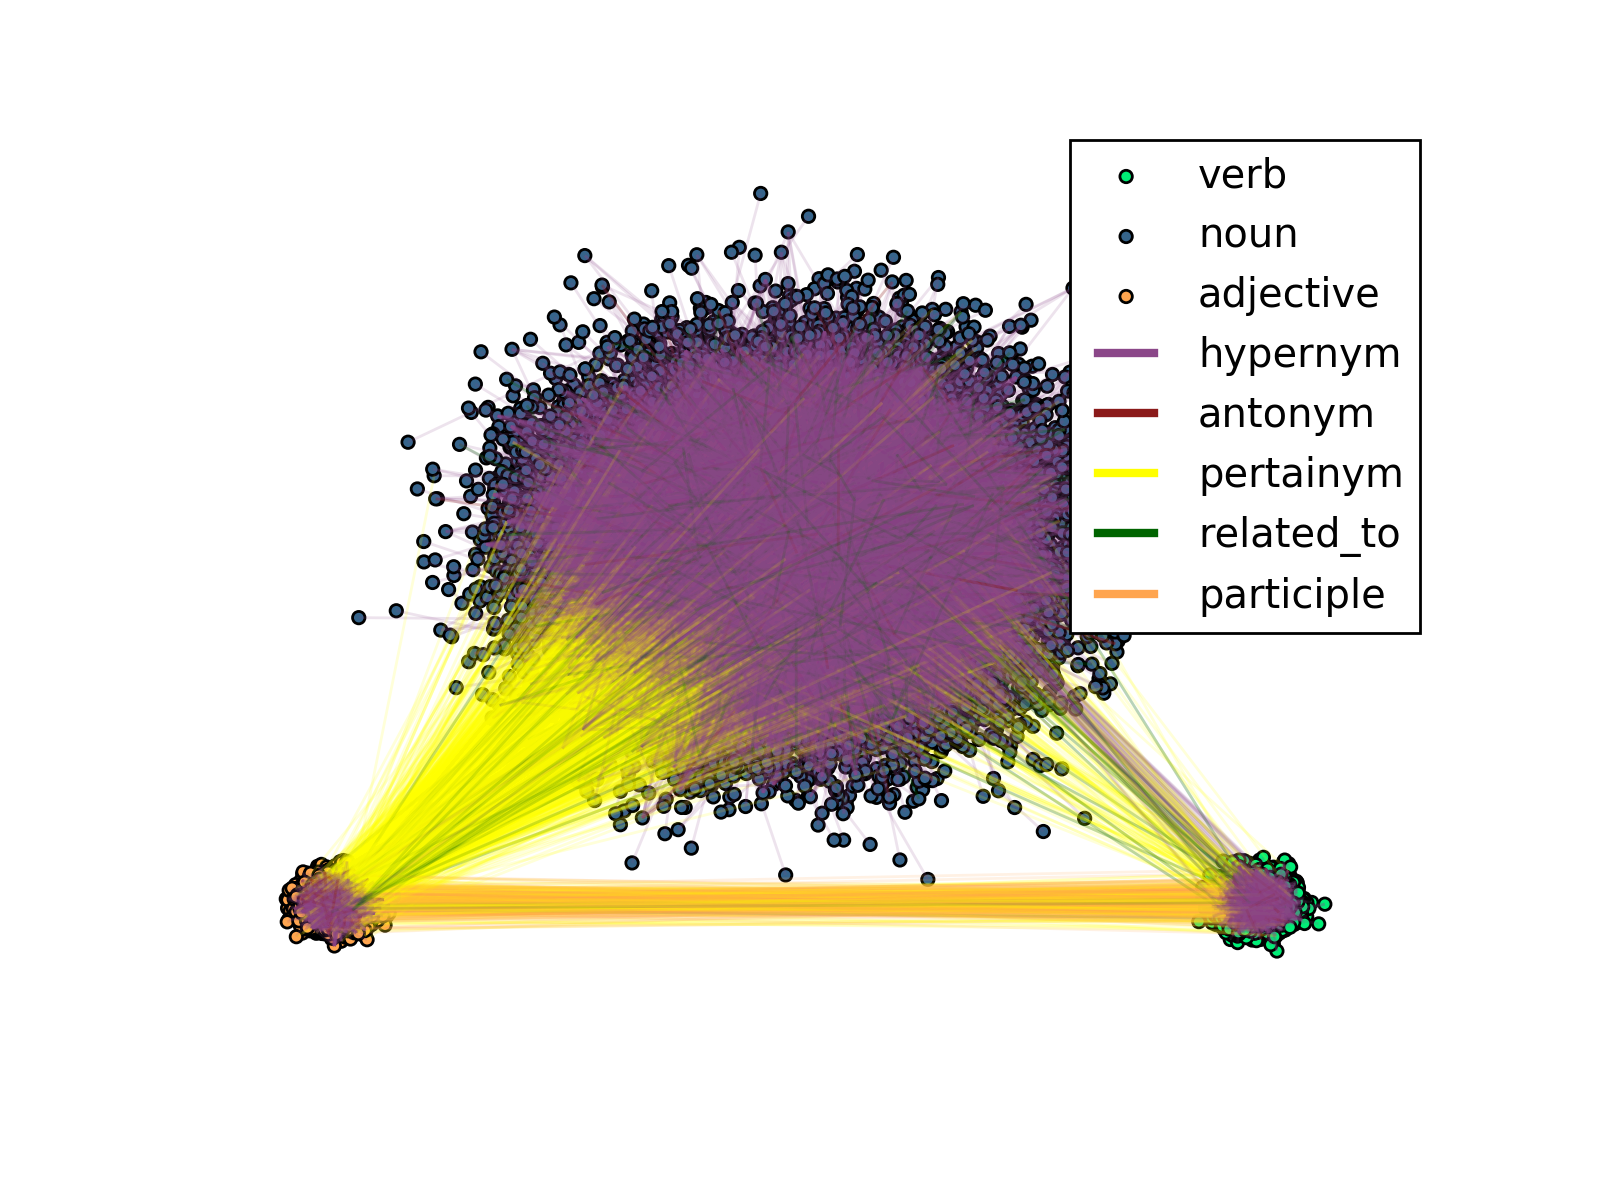
\includegraphics[width=\linewidth]{img/germanet.png}
%   \caption{\textsc{GermaNet}}\label{snt-lex:fig:germanet}
% \end{subfigure}%
% \begin{subfigure}{.5\textwidth}
%   \centering
%   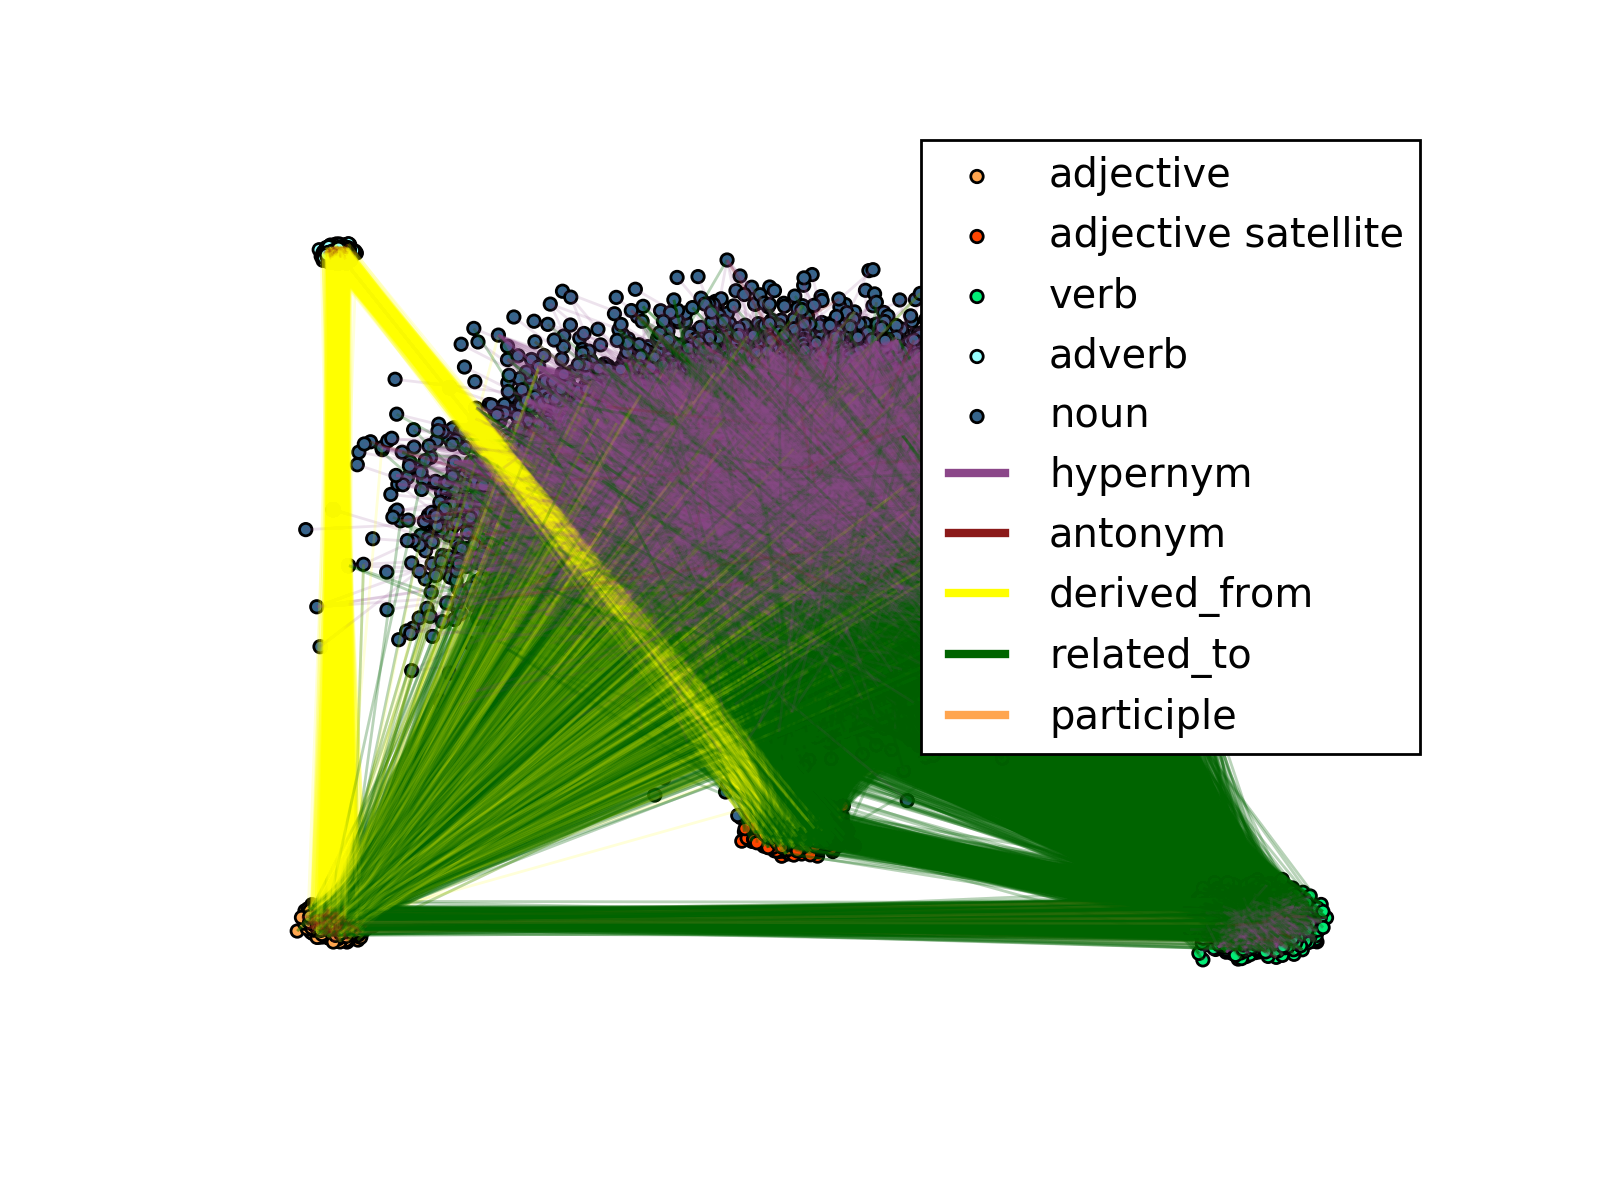
\includegraphics[width=\linewidth]{img/wordnet.png}
%   \caption{\textsc{WordNet}}\label{snt-lex:fig:wordnet}
% \end{subfigure}
% }
% \caption{Graphical visualization of \textsc{GermaNet} and
%       \textsc{WordNet}.}\label{snt:fig:crp-sent-emo-distr}
% \end{figure*}

% As can be seen from the table, \textsc{GermaNet} has significantly
% fewer words and synsets for all common parts of speech with the
% largest gaps observed for nouns and adjectives.  Moreover, as shown in
% Figures~\ref{snt-lex:fig:germanet} and~\ref{snt-lex:fig:wordnet}, such
% PoS-classes as adverbs and adjective satellites are completely missing
% in the German resource.  The reason for this is that the form (and
% meaning) of most German adverbs typically coincides with that of the
% adjectives; therefore, both categories are treated in the same way,
% being represented through the adjectival synsets.

% A slightly different situation can be observed for the semantic links
% (relations) between the synsets: here, \textsc{GermaNet} features
% almost 2,500 more hypernym-hyponym pairs than the English resource,
% whereas the number of antonyms is more than four times less than in
% \textsc{WordNet}.

% An especially interesting pattern, however, appears with the relations
% connecting different parts of speech: As can be seen from the figures,
% the strongest inter-PoS connections in \textsc{GermaNet} are the
% pertainym links between the adjectives and nouns and the participle
% edges between the adjectives and verbs.  The interlinks between the
% nouns and verbs, however, are both much fewer in number and more
% diverse in their nature.  This situation is different in
% \textsc{WordNet} where the prevailing majority of the
% inter-part-of-speech connections are represented through the
% \texttt{related\_to} (especially between the nouns, adjective
% satellites, verbs, and verbs and adjectives) and
% \texttt{derived\_from} links (especially between adverbs and
% adjectives with their satellites).  The relations between the
% adjectives and nouns are mixed though, featuring both
% \texttt{related\_to} and \texttt{derived\_from} connections.  As we
% should see later, these links are crucial for breaking part-of-speech
% dependencies of seed sets in the cases when all seeds belong to the
% same PoS class.

% Another lexical sentiment resource (\textsc{WordNet-Affect}) was
% proposed by \citet{Strapparava:04} who manually compiled a list of
% 1,903 subjective terms and projected these polarities to the
% respective synononyms set in \textsc{WordNet}.  The resulting database
% included 2,874 synsets with a total of 4,787 words.

% \subsection{Domain-Specific Sentiment Lexicons}

% \citet{Chetviorkin:14} obtained a set of possible subjective terms
% from English and Russian microblogs by using an ensemble of supervised
% machine learning classifiers that had previously been trained on a
% manually annotated corpus of movie reviews.  In order to determine the
% prior polarity of the extracted terms, the authors first calculated
% approximate polarity scores of the processed messages using general
% polarity lexicons and then took these rough estimates as prior
% polarity expectations of the candidate expressions.  The posterior
% scores of these expressions were computed using the Ising spin model
% in a similar way to the approach proposed by \citet{Takamura:05}.  The
% resulting lexicon comprised 2,772 words for Russian and 2,786 lexical
% items for English.

\section{Summary and Conclusions}

Concluding this chapter, we would like to recapitulate that, in this
part, we presented a thorough review of the most popular sentiment
lexicon generation methods.  For this purpose, we first revised
existing SL evaluation techniques, also suggesting our own (stricter)
way of estimating the quality of such resources.  With this proposed
metric, we explicitly counted all false positive, false negative, and
true positive occurrences of positive, negative, and neutral terms on
a real-life sentiment corpus, and also computed the macro- and
micro-averaged \F-scores of these polarity classes.  Using our
procedure, we first evaluated the most popular semi-automatic German
lexicons: the German Polarity Clues of~\citet{Waltinger:10}, the
SentiWS lexicon of~\citet{Remus:10}, and the Zurich Polarity List
of~\citet{Clematide:10}, finding the last resource working best in
terms of the macro-averaged results.  Afterwards, we estimated the
quality of automatically induced polarity lists that were created with
either dictionary- or corpus-based SLG approaches, coming to the
conclusion that the former group of methods generally produced much
better lexicons, and was less susceptible to the contentual noisiness
of the Twitter domain.  In the next step, we introduced several novel
SLG approaches which operated on neural embeddings of words, showing
that at least two of them (the method of $k$ nearest neighbors and the
linear projection system) outperformed all other compared automatic
SLG algorithms.  Last but not least, we explored the effect of
different hyper-parameters and settings on the net results of these
methods, rerunning them with alternative sets of initial seed terms,
checking their performance on different kinds of embeddings, and
estimating the impact of various vector normalization techniques.

Based on our observations and experiments, we can formulate the main
conclusions and contributions of this part of the thesis as follows:
\begin{itemize}
\item semi-automatic translations of common English polarity lists
  notably outperform purely automatic SLG methods which are applied to
  German data directly;
\item despite their allegedly worse ability to accommodate new
  domains, dictionary-based approaches are still superior to
  corpus-based systems (at least in terms of an intrinsic evaluation);
\item a potential weakness of these algorithms though is their
  dependence on various types of hyper-parameters and the existence of
  rich manually annotated linguistic resources, which might not
  necessarily be present for every language;
\item in this regard, a viable alternative to dictionary-based methods
  are SLG systems which induce polar lexicons from neural word
  embeddings as they not only avoid the above limitations, but also
  yield competitive (or even better) results;
\item with at least two of such methods ($k$-NN and linear
  projection), we were able to establish a new state of the art for
  the macro- and micro-averaged \F-scores of automatically induced
  sentiment lexicons;
\item furthermore, an extensive evaluation of various sets of seed
  terms revealed that the results of almost all tested SLG algorithms
  crucially depended on the quality of their initial seeds, with
  larger balanced seed sets, e.g, like the one proposed
  by~\citet{Kim:04}, typically leading to much higher scores;
\item we also checked how different types of embeddings were affecting
  the performance of NWE-based SLG systems, noticing that the $k$-NN
  and linear projection methods worked best with the standard word2vec
  vectors, while the nearest centroids and PCA algorithms yielded
  better results on task-specific representations;
\item finally, we saw that all NWE-based approaches benefited from the
  mean-scaling and length normalization of the input vectors, getting
  an improvement by up to~5\% in their macro-averaged \F-scores.
\end{itemize}

With this knowledge in mind, we will now move on to exploring further
opinion mining fields: fine- and coarse-grained sentiment analysis, in
which sentiment lexicons are traditionally considered to be one of the
most fundamental building blocks.
